% ======================================================================
%  Formation de la Lune -- Théorie du disque secondaire circumterrestre
%  Une théorie de chemin rétrodictive du système proto-terrestre au système Terre--Lune
%  Michel Debailleul — © 2026 — Licence CC BY-NC 4.0
%  Compilation : pdflatex (trois passes pour la table des matières et les renvois)
% ======================================================================
\documentclass[11pt,a4paper,openany]{report}

\usepackage[utf8]{inputenc}
\usepackage[T1]{fontenc}
\usepackage{lmodern}
\usepackage[french]{babel}
\usepackage{amsmath,amssymb}
\usepackage[a4paper,margin=2.4cm,headheight=14pt]{geometry}
\usepackage{microtype}
\usepackage{booktabs,array,tabularx,longtable}
\usepackage{xcolor}
\usepackage{graphicx}
\graphicspath{{./}{../figures/}}
\usepackage[most]{tcolorbox}
\usepackage{tikz}
\usetikzlibrary{arrows.meta,calc,positioning,decorations.pathmorphing,babel}
\usepackage{pgfplots}
\usepgfplotslibrary{fillbetween}
\pgfplotsset{compat=1.18}
\usepackage{titlesec}
\usepackage{fancyhdr}
\usepackage{hyperref}
\hypersetup{
  colorlinks=true,
  linkcolor=blue!45!black,
  citecolor=blue!45!black,
  urlcolor=blue!45!black,
  pdftitle={Formation de la Lune -- Théorie du disque secondaire circumterrestre},
  pdfauthor={Michel Debailleul},
  pdfsubject={Une théorie de chemin rétrodictive du système proto-terrestre au système Terre--Lune},
  pdfkeywords={Lune, disque circumterrestre, accrétion secondaire, rencontre non collisionnelle,
  moment cinétique, tri orbital, géochimie lunaire, instabilité orbitale primitive, planète éliminée}
}

% ---------------------------------------------------------------------
%  Titres de parties et de chapitres
% ---------------------------------------------------------------------
\titleclass{\part}{top}
\titleformat{\part}[display]
  {\centering\normalfont\bfseries\color{blue!40!black}}
  {\Large\partname~\thepart}{10pt}{\Huge}
\titlespacing*{\part}{0pt}{30pt}{28pt}
\titleformat{\chapter}[display]
  {\normalfont\bfseries}{\large\chaptertitlename~\thechapter}{6pt}{\LARGE}
\titlespacing*{\chapter}{0pt}{-8pt}{18pt}

% ---------------------------------------------------------------------
%  Encadrés
% ---------------------------------------------------------------------
\tcbset{boite/.style={enhanced,breakable,boxrule=0.6pt,arc=2pt,
  left=6pt,right=6pt,top=4pt,bottom=4pt,fonttitle=\bfseries\small,
  before skip=8pt,after skip=10pt}}
\newtcolorbox{ideephys}{boite,colback=blue!3,colframe=blue!45!black,title=Idée physique}
\newtcolorbox{lecture}{boite,colback=teal!3,colframe=teal!55!black,title=Lecture physique}
\newtcolorbox{falsif}{boite,colback=red!3,colframe=red!55!black,title=Critère de falsification}
\newtcolorbox{controle}{boite,colback=orange!4,colframe=orange!70!black,title=Contrôle quantitatif}
\newtcolorbox{apport}{boite,colback=violet!4,colframe=violet!65!black,title=Apport original de la théorie}
\newtcolorbox{consequence}{boite,colback=green!4,colframe=green!40!black,title=Conséquence observable}
\newtcolorbox{definition}{boite,colback=brown!5,colframe=brown!65!black,title=Définition}
\newtcolorbox{rappel}{boite,colback=gray!5,colframe=gray!60!black,title=Rappel didactique}
\newtcolorbox{principe}[1]{boite,colback=gray!4,colframe=gray!55!black,title=#1}
\newtcolorbox{prediction}[1]{boite,colback=cyan!3,colframe=cyan!40!black,title=Prédiction --- #1}
\newcommand{\sila}{\par\noindent\textbf{Si la théorie est correcte.}\ }
\newcommand{\verif}{\par\smallskip\noindent\textbf{Comment la vérifier.}\ }

% ---------------------------------------------------------------------
%  Notations
% ---------------------------------------------------------------------
\newcommand{\Mt}{M_{\oplus}}
\newcommand{\Rt}{R_{\oplus}}
\newcommand{\Req}{R_{\mathrm{eq}}}
\newcommand{\aR}{a_{\mathrm{Roche}}}
\newcommand{\dd}{\mathrm{d}}
\newcommand{\Mtot}{M_{\mathrm{tot}}}
\newcommand{\RT}{\mathcal{R}_{\oplus}}
\newcommand{\RD}{\mathcal{R}_{D}}
\newcommand{\RB}{\mathcal{R}_{B}}
\newcommand{\Rinf}{\mathcal{R}_{\infty}}

% ---------------------------------------------------------------------
%  En-têtes
% ---------------------------------------------------------------------
\pagestyle{fancy}
\fancyhf{}
\fancyhead[L]{\small\nouppercase{\leftmark}}
\fancyhead[R]{\small Michel Debailleul}
\fancyfoot[C]{\small\thepage}
\renewcommand{\headrulewidth}{0.4pt}
\fancypagestyle{plain}{\fancyhf{}\fancyfoot[C]{\small\thepage}\renewcommand{\headrulewidth}{0pt}}

\begin{document}

% =====================================================================
%  PAGE DE TITRE
% =====================================================================
\pagenumbering{Alph}
\begin{titlepage}
\thispagestyle{empty}
\centering
\vspace*{0.8cm}
{\LARGE\bfseries Formation de la Lune\\[4pt] Théorie du disque secondaire circumterrestre\par}
\vspace{0.45cm}
{\Large Une théorie de chemin rétrodictive\\ du système proto-terrestre au système Terre--Lune\par}
\vspace{0.35cm}
{\normalsize Réservoirs, flux, passage planétaire non collisionnel,\\
géochimie et domaine de viabilité\par}
\vspace{1.1cm}

\begin{tikzpicture}[scale=1.05]
  \fill[blue!30,opacity=0.55,even odd rule] (0,0) ellipse (3.5 and 0.62) (0,0) ellipse (1.25 and 0.22);
  \shade[ball color=orange!75!brown] (0,0) ellipse (1.02 and 0.9);
  \begin{scope}
    \clip (-4,-1.2) rectangle (4,0);
    \fill[blue!30,opacity=0.55,even odd rule] (0,0) ellipse (3.5 and 0.62) (0,0) ellipse (1.25 and 0.22);
  \end{scope}
  \draw[dashed,thick,gray!60!black,-{Stealth[length=3mm]}]
      (6.2,3.5) .. controls (2.0,2.3) and (2.0,1.3) .. (6.2,-0.1);
  \shade[ball color=gray!55] (3.0,1.72) circle (0.38);
  \node[font=\small] at (2.15,2.2) {planète $B$};
  \node[font=\small] at (0,-1.35) {proto-Terre};
  \node[font=\small,blue!45!black] at (-2.9,0.95) {disque secondaire};
  \draw[->,thick,red!60!black] (2.55,1.45) -- (1.5,0.75);
  \node[font=\scriptsize,red!60!black,align=center] at (1.35,1.55) {couple\\gravitationnel};
\end{tikzpicture}

\vspace{1.2cm}
{\large\bfseries Michel Debailleul\par}
\vspace{0.15cm}
Géophysicien, Chercheur Indépendant --- Université libre de Bruxelles (ULB)\\
ORCID : 0009-0003-1222-1433 \quad | \quad \href{mailto:michel.debailleul@yahoo.fr}{michel.debailleul@yahoo.fr}\\[4pt]
\copyright\ 2026 Michel Debailleul --- Licence : CC BY-NC 4.0
\vfill
\end{titlepage}
\pagenumbering{roman}

% =====================================================================
%  RÉSUMÉ / ABSTRACT
% =====================================================================
\thispagestyle{plain}
\begin{center}{\Large\bfseries Résumé}\end{center}
\medskip

Le système Terre--Lune présente aujourd'hui une architecture dynamique, une distribution de
masse, un moment cinétique, des signatures isotopiques, des compositions géochimiques et une
chronologie qui constituent autant de contraintes observationnelles indépendantes. La question
traitée ici n'est pas de décrire ces propriétés, mais d'identifier un \emph{chemin physique}
continu reliant l'état initial du système proto-terrestre à l'état observé.

L'ancrage astrophysique de cette démarche est que des satellites naturels sont déjà interprétés
comme les produits de réservoirs circumplanétaires : les satellites réguliers de Jupiter et de
Saturne dans des disques circumplanétaires, et les satellites internes de Neptune dans un système
remanié où un disque de débris aurait suivi la capture de Triton. Le cas terrestre proposé ne
transpose pas leurs masses ni leurs compositions ; il reprend le principe physique d'un réservoir
lié à une planète, capable de transporter masse et moment cinétique puis de former des satellites.

Cet ouvrage explore un tel chemin. Un disque secondaire circumterrestre, contemporain de
l'accrétion de la proto-Terre, constitue un réservoir orbital de masse et de moment cinétique
avant la formation de la Lune. Une planète $B$, en passage rasant et non collisionnel, n'est ni un
impacteur ni un fournisseur principal de matière lunaire : elle agit comme un \emph{agent
gravitationnel transitoire de redistribution des flux de masse et de moment cinétique} entre
quatre réservoirs --- la proto-Terre, le disque, la planète $B$ et le milieu extérieur.

La logique héliocentrique du modèle est que $B$ n'a pas à subsister dans le Système solaire
actuel. Elle peut appartenir à la population des corps planétaires primitifs ensuite éliminés par
l'instabilité orbitale globale du Système solaire. Cette extension ne l'identifie pas nécessairement
à une cinquième géante de glace ; elle exige seulement que son passage rasant précède son
élimination dynamique, selon la condition $t_B<t_{\mathrm{ej}}$. Elle relie ainsi le problème
Terre--Lune à celui, plus général, de la migration et de l'instabilité planétaires primitives
\cite{Tsiganis2005,Gomes2005,Nesvorny2011,NesvornyMorbidelli2012,Liu2022,Clement2018}.

Le passage réalise un tri orbital. Une cohorte de matière liée acquiert un moment cinétique qui
la place, après circularisation, au-delà de la limite de Roche, dans la fenêtre où la Lune peut
s'accréter ; une fraction réaccrète sur la proto-Terre, une autre s'échappe. Un passage parallèle
à la bande dynamique de basses latitudes d'une proto-Terre oblate en rotation rapide peut
en outre injecter dans
le disque une matière superficielle déjà appauvrie en métal et en éléments sidérophiles, dont les
traceurs W, V, Cr, Mn, FeO, O et Ti permettent de tester la lignée.

L'ouvrage formule successivement le problème scientifique, les fondements astrophysiques,
l'architecture des réservoirs, la chronologie physique, la dynamique du passage, l'évolution du
réservoir circumterrestre, la géochimie par familles de traceurs, le domaine de viabilité et les
prédictions, chacune accompagnée de sa méthode de vérification. Il ne prétend pas démontrer
une histoire unique : il définit un chemin physique quantitatif et falsifiable.

\bigskip
\noindent\textbf{Mots-clés :} formation de la Lune ; disque circumterrestre ; accrétion secondaire ;
rencontre non collisionnelle ; tri orbital ; moment cinétique ; limite de Roche ; géochimie lunaire ; instabilité orbitale primitive ; planète éliminée.

\bigskip
\begin{otherlanguage}{english}
\begin{center}{\Large\bfseries Abstract}\end{center}
\medskip

The Earth--Moon system currently exhibits a dynamical architecture, a mass distribution, an
angular momentum, isotopic signatures, geochemical compositions and a chronology that together
form independent observational constraints. The question addressed here is not to describe these
properties, but to identify a continuous \emph{physical path} linking the initial state of the
proto-terrestrial system to the observed state.

The astrophysical anchor of this approach is that natural satellites are already interpreted as
the products of circumplanetary reservoirs: the regular satellites of Jupiter and Saturn in
circumplanetary disks, and the inner satellites of Neptune in a reworked system where a debris
disk probably followed the capture of Triton. The proposed terrestrial case does not import their
masses or compositions; it retains the physical principle of a reservoir bound to a planet, able
to transport mass and angular momentum and then to form satellites.

This work explores such a path. A secondary circumterrestrial disk, contemporaneous with the
accretion of the proto-Earth, forms an orbital reservoir of mass and angular momentum before the
Moon forms. A planet $B$, on a grazing and non-collisional passage, is neither an impactor nor the
main supplier of lunar material: it acts as a \emph{transient gravitational agent redistributing
mass and angular-momentum fluxes} between four reservoirs --- the proto-Earth, the disk, planet
$B$ and the external medium.

The heliocentric logic of the model is that $B$ need not survive in the present Solar System. It may
belong to the population of primordial planetary bodies later eliminated by the global orbital
instability of the Solar System. This extension does not necessarily identify it with a fifth ice
giant; it only requires its grazing passage to precede its dynamical elimination, according to
$t_B<t_{\mathrm{ej}}$. It thus links the Earth--Moon problem to the broader problem of primordial
planetary migration and instability
\cite{Tsiganis2005,Gomes2005,Nesvorny2011,NesvornyMorbidelli2012,Liu2022,Clement2018}.

The passage performs an orbital sorting. A bound cohort of matter acquires an angular momentum
that places it, after circularization, beyond the Roche limit, in the window where the Moon can
accrete; one fraction re-accretes onto the proto-Earth, another escapes. A passage parallel to the
dynamical low-latitude band of an oblate rapidly rotating proto-Earth can also inject into the disk
surface material already depleted in metal and siderophile elements; W, V, Cr, Mn, FeO, O and Ti
then provide tracers with which to test the lineage.

The work successively formulates the scientific problem, the astrophysical foundations, the
reservoir architecture, the physical chronology, the passage dynamics, the evolution of the
circumterrestrial reservoir, geochemistry by tracer families, the viability domain and the
predictions, each with a verification method. It does not claim to prove a unique history: it
defines a quantitative and falsifiable physical path.

\bigskip
\noindent\textbf{Keywords:} Moon formation; circumterrestrial disk; secondary accretion;
non-collisional encounter; orbital sorting; angular momentum; Roche limit; lunar geochemistry; primordial orbital instability; eliminated planet.
\end{otherlanguage}

% =====================================================================
%  PRÉAMBULE MÉTHODOLOGIQUE
% =====================================================================
\clearpage
\thispagestyle{plain}
\phantomsection
\addcontentsline{toc}{chapter}{Préambule méthodologique}
\begin{center}
{\Large\bfseries Préambule méthodologique}\\[4pt]
{\large\bfseries Une théorie de chemin rétrodictive}
\end{center}
\medskip

La présente monographie ne prétend pas reconstruire de manière unique ce qui
s'est réellement produit dans l'histoire du Système solaire. Une telle
reconstruction serait probablement inaccessible : les conditions initiales
exactes du système proto-terrestre, les trajectoires individuelles des corps
planétaires, l'état thermodynamique détaillé des réservoirs et la chronologie
fine des rencontres ont disparu.

L'objectif est différent. Il s'agit de construire un \emph{chemin physique
possible} reliant un système proto-terrestre admissible au système Terre--Lune
observé. La démarche est donc rétrodictive : elle part de l'état final connu,
puis remonte, contrainte après contrainte, vers une famille d'états initiaux et
d'étapes dynamiques capables de produire cet état final.

Le problème traité n'est donc pas :

\begin{center}
\emph{Quel événement unique s'est réellement produit ?}
\end{center}

mais plutôt :

\begin{center}
\emph{Existe-t-il un chemin physique continu, quantitativement contraint et
falsifiable, reliant un état proto-terrestre possible à l'état Terre--Lune
observé ?}
\end{center}

Ce statut peut s'écrire sous la forme
\begin{equation}
\boxed{
\exists\,\Gamma(t)\in\mathcal{D}_{\mathrm{viable}}
\quad\text{tel que}\quad
\Gamma(t_0)=\mathcal{S}_0,\qquad
\Gamma(t_f)=\mathcal{S}_f .
}
\label{eq:statut-retrodictif}
\end{equation}

La trajectoire $\Gamma(t)$ ne désigne pas nécessairement l'histoire réelle du
Système solaire. Elle désigne un chemin admissible dans l'espace des états
physiques : masse, moment cinétique, énergie, composition, phases de la matière
et chronologie. La valeur scientifique de la théorie ne repose donc pas sur une
revendication d'unicité historique, mais sur l'existence éventuelle d'un domaine
continu de paramètres satisfaisant simultanément les contraintes dynamiques,
géochimiques, isotopiques, thermodynamiques et chronologiques.

Dans ce cadre, le disque secondaire circumterrestre n'est pas introduit comme
un artifice narratif, mais comme un réservoir physique à tester. De même, la
planète $B$ n'est ni un impacteur ni un fournisseur principal de matière
lunaire : elle est un agent gravitationnel transitoire de redistribution des
flux de masse et de moment cinétique. Son destin ultérieur appartient au même
cadre rétrodictif. Elle peut appartenir à la population des corps planétaires du
Système solaire primitif ensuite éliminés par collision, accrétion, diffusion
gravitationnelle ou éjection.

La condition minimale associée à cette extension héliocentrique est
\begin{equation}
\boxed{
B\in\mathcal{P}_{\mathrm{elim}},
\qquad
 t_B<t_{\mathrm{ej}} .
}
\label{eq:B-elim-preambule}
\end{equation}

Ici, $\mathcal{P}_{\mathrm{elim}}$ désigne la population des corps planétaires
présents dans le Système solaire primitif mais absents du système actuel ;
$t_B$ est l'instant du passage rasant près de la proto-Terre ; et
$t_{\mathrm{ej}}$ l'instant de l'élimination dynamique de $B$. Cette formulation
laisse ouvertes les deux possibilités : une instabilité orbitale précoce ou une
instabilité plus tardive.

\begin{principe}{Statut de la théorie}
La théorie du disque secondaire circumterrestre est une théorie de chemin, non
une revendication d'unicité historique. Elle devient crédible si un domaine
continu de paramètres permet de franchir ensemble les portes dynamiques,
géochimiques, isotopiques, thermodynamiques et chronologiques. Elle devient
falsifiée si aucun tel domaine n'existe.
\end{principe}

% =====================================================================
%  GUIDE DE LECTURE
% =====================================================================
\clearpage
\thispagestyle{plain}
\begin{center}{\Large\bfseries Guide de lecture}\end{center}
\medskip

L'ouvrage est construit pour être lu, et pas seulement consulté. Chaque partie commence par une
présentation de sa question et se termine par le lien avec la suivante. Les démonstrations
longues sont regroupées en annexe~\ref{app:demo}, afin que le corps du texte reste continu ; les
notations sont rassemblées en annexe~\ref{app:notations} et les valeurs numériques en
annexe~\ref{app:constantes}.

Des encadrés de types distincts balisent la lecture :

\begin{definition}
Fixe le sens d'un terme ou d'un rôle, qui devient la référence pour tout l'ouvrage.
\end{definition}
\begin{ideephys}
Donne l'intuition physique qui se cache derrière un calcul.
\end{ideephys}
\begin{lecture}
Interprète une équation ou un résultat dans le cadre du chemin physique.
\end{lecture}
\begin{rappel}
Rappelle une notion classique utile à la compréhension.
\end{rappel}
\begin{controle}
Confronte un résultat à des ordres de grandeur ou à un bilan de conservation.
\end{controle}
\begin{consequence}
Indique ce que l'on devrait observer, dans les échantillons lunaires ou dans les simulations,
si le mécanisme décrit est à l'\oe uvre.
\end{consequence}
\begin{falsif}
Énonce la condition sous laquelle une branche de la théorie doit être abandonnée.
\end{falsif}
\begin{apport}
Signale ce qui distingue la théorie des scénarios existants.
\end{apport}

\clearpage
\tableofcontents

% =====================================================================
\clearpage
\pagenumbering{arabic}
\part{Le problème scientifique}
% =====================================================================

\noindent
Cette première partie pose la question à laquelle l'ouvrage répond. Elle ne commence ni par le
disque ni par la planète $B$, mais par le système Terre--Lune tel qu'il est observé, et par
l'exigence que ces observations imposent à toute histoire de sa formation. Elle établit aussi un
point d'ancrage essentiel : la nature connaît déjà des satellites issus de réservoirs
circumplanétaires. Le disque secondaire, la planète $B$, les flux entre réservoirs, la géochimie
et la dynamique apparaissent ensuite comme les éléments d'une même réponse.

% ---------------------------------------------------------------------
\chapter{Du système proto-terrestre au système Terre--Lune}
\label{ch:probleme}
% ---------------------------------------------------------------------

\section{Le problème scientifique}

La Lune existe. Le système Terre--Lune présente aujourd'hui une architecture dynamique, une
distribution de masse, un moment cinétique, des signatures isotopiques, des compositions
géochimiques et une chronologie qui constituent autant de contraintes observationnelles
indépendantes.

Ces observations sont désormais suffisamment nombreuses et suffisamment précises pour
imposer un cadre physique exigeant à toute théorie de la formation lunaire. Aucune de ces
contraintes ne peut être considérée isolément : la dynamique orbitale, la géochimie, les
systèmes isotopiques, la thermodynamique et la chronologie décrivent un même système
physique et doivent pouvoir être expliquées de manière cohérente.

La question scientifique n'est donc pas de savoir si la Lune existe ni quelles sont aujourd'hui
ses propriétés, mais de déterminer :

\begin{center}
\emph{Quel chemin physique a conduit naturellement du système proto-terrestre\\ au système
Terre--Lune actuellement observé ?}
\end{center}

Autrement dit, il s'agit d'identifier une évolution physiquement admissible reliant un état
initial de la proto-Terre à l'état final représenté par le système Terre--Lune, tout en respectant
simultanément les contraintes imposées par les observations. Cette démarche se représente de
manière générale par
\begin{equation}
\boxed{\;\mathcal{S}_0\longrightarrow\mathcal{S}_f\;}
\label{eq:S0Sf}
\end{equation}
où $\mathcal{S}_0$ désigne l'état initial du système proto-terrestre et $\mathcal{S}_f$ l'état
actuellement observé. Le problème scientifique consiste à déterminer s'il existe un chemin
physique continu reliant ces deux états.

\begin{figure}[htbp]
\centering
\begin{tikzpicture}[node distance=0.45cm,
  st/.style={draw,rounded corners=3pt,align=center,font=\small,minimum height=1.15cm,
             text width=2.25cm,fill=#1},
  st/.default=white,
  ts/.style={draw,dashed,rounded corners=2pt,align=center,font=\scriptsize,text width=2.25cm,
             fill=green!4}]
  \node[st=blue!8] (s0) {$\mathcal{S}_0$\\proto-Terre\\+ réservoir $\RD$};
  \node[st=violet!10,right=of s0] (s1) {passage\\non collisionnel\\de $B$};
  \node[st=blue!8,right=of s1] (s2) {réservoir\\réorganisé\\(tri orbital)};
  \node[st=teal!8,right=of s2] (s3) {accrétion\\lunaire};
  \node[st=orange!10,right=of s3] (sf) {$\mathcal{S}_f$\\système\\Terre--Lune};
  \foreach \a/\b in {s0/s1,s1/s2,s2/s3,s3/sf} \draw[-{Stealth},thick] (\a) -- (\b);
  \node[ts,below=0.9cm of s1] (t1) {moment cinétique\\et masse};
  \node[ts,below=0.9cm of s2] (t2) {dynamique\\et architecture};
  \node[ts,below=0.9cm of s3] (t3) {géochimie\\et isotopes};
  \node[ts,below=0.9cm of sf] (t4) {chronologie};
  \foreach \t/\s in {t1/s1,t2/s2,t3/s3,t4/sf} \draw[-{Stealth},dashed,green!40!black] (\t) -- (\s);
  \node[font=\scriptsize,green!40!black,anchor=east] at ($(t1.west)+(-0.1,0)$) {tests indépendants};
\end{tikzpicture}
\caption{Le problème posé comme la recherche d'un chemin physique continu entre l'état initial
$\mathcal{S}_0$ et l'état observé $\mathcal{S}_f$. Chaque famille d'observations teste le chemin de
façon indépendante.}
\label{fig:chemin}
\end{figure}

\section{Les contraintes observationnelles}

Le tableau~\ref{tab:contraintes} rassemble les familles de contraintes que le chemin doit
satisfaire simultanément. Elles serviront, dans la partie~\ref{part:predictions}, de tests
indépendants.

\begin{table}[htbp]
\centering
\small
\caption{Familles de contraintes observationnelles imposées au chemin physique.}
\label{tab:contraintes}
\begin{tabularx}{\textwidth}{>{\raggedright\arraybackslash}p{2.6cm}
>{\raggedright\arraybackslash}X >{\raggedright\arraybackslash}p{5.4cm}}
\toprule
\textbf{Famille} & \textbf{Contrainte} & \textbf{Nature ou ordre de grandeur} \\
\midrule
Masse & rapport $M_L/\Mt$ & $1{,}23\times10^{-2}$ \\
Architecture & un satellite dominant & $f_{\mathrm{dom}}\simeq1$ \\
Moment cinétique & moment total du système & $L_{\mathrm{EM}}\approx3{,}5\times10^{34}$ kg\,m$^2$\,s$^{-1}$ \\
Orbite & inclinaison orbitale lunaire & environ $5^\circ$ sur l'écliptique \\
Structure interne & petit noyau lunaire & quelques pour cent de la masse au plus \\
Isotopes & O, Ti, Cr, W & Terre et Lune très proches, souvent indiscernables \\
Sidérophiles & V, Cr, Mn, W & appauvrissements semblables à ceux du manteau terrestre \\
Fer & FeO du manteau lunaire & plus élevé que dans le manteau terrestre \\
Volatils & K/U, Zn, isotopes & Lune appauvrie en éléments volatils \\
Chronologie & âge de formation & plusieurs dizaines de millions d'années après les premiers solides \\
\bottomrule
\end{tabularx}
\end{table}


\section{Ancrage astrophysique : des satellites naturels issus de disques}

Avant d'introduire le cas terrestre, un fait astrophysique doit être posé clairement : la formation
de satellites à partir d'un réservoir circumplanétaire n'est pas une construction ad hoc. Dans le
Système solaire, plusieurs familles de satellites naturels sont interprétées comme les produits
d'une matière liée à une planète, organisée dans un disque, un anneau massif ou un disque de
débris, puis transformée en satellites par accrétion, migration, dissipation et franchissement de
la limite de Roche.

\begin{principe}{Ancrage observationnel}
La théorie ne part pas de l'idée abstraite qu'un disque pourrait former une Lune. Elle part d'un
principe observé à plusieurs reprises :
\begin{equation}
\boxed{\;\text{planète en croissance ou remaniée}+\text{réservoir circumplanétaire}
\longrightarrow \text{satellites naturels}.\;}
\label{eq:ancrage-satellites}
\end{equation}
Le cas terrestre doit ensuite être traité avec ses propres contraintes : une planète tellurique,
un réservoir dominé par les solides, une masse lunaire élevée et un passage non collisionnel de
$B$ jouant le rôle d'agent de redistribution.
\end{principe}

Trois exemples jouent un rôle particulier dans le raisonnement. Le système galiléen de Jupiter
constitue l'exemple le plus classique d'un système régulier dont la formation est liée à un disque
circumjovien alimenté pendant la croissance de la planète. Les modèles discutent l'influx de gaz
et de solides, le transport de moment cinétique, la migration et les conditions d'accrétion des
satellites \cite{CanupWard2002,MosqueiraEstrada2003a,CanupWard2006,Nimmo2026}. Saturne apporte
un second appui : ses satellites réguliers et son système d'anneaux montrent qu'un réservoir
circumplanétaire peut transporter de la matière, s'étaler visqueusement, franchir la limite de
Roche et former des satellites \cite{Charnoz2010,CridaCharnoz2012,Blanc2025}. Neptune enfin est
un cas plus subtil : Triton est très probablement capturé, mais son arrivée a pu détruire ou
remanier un système régulier antérieur et produire un disque de débris à partir duquel les
satellites internes actuels se sont reformés ou réaccrétés
\cite{AgnorHamilton2006,BanfieldMurray1992,Showalter2019,Szulagyi2018,Davis2026}.

\begin{table}[htbp]
\centering
\small
\caption{Exemples naturels montrant qu'un réservoir circumplanétaire peut former ou reformer des
satellites. Ces exemples établissent le principe physique ; ils ne fixent pas les paramètres du
cas terrestre.}
\label{tab:ancrage-satellites}
\begin{tabularx}{\textwidth}{>{\raggedright\arraybackslash}p{2.4cm}
>{\raggedright\arraybackslash}X >{\raggedright\arraybackslash}X}
\toprule
\textbf{Système} & \textbf{Réservoir ou processus invoqué} & \textbf{Leçon physique pour le chemin proposé} \\
\midrule
Jupiter & disque circumjovien alimenté en gaz et solides pendant la croissance de Jupiter &
un disque circumplanétaire peut produire plusieurs satellites réguliers organisés \\
Saturne & disque circumplanétaire, anneaux massifs, étalement visqueux et franchissement de Roche &
un réservoir particulaire peut migrer, franchir Roche et alimenter une accrétion satellitaire \\
Neptune & capture de Triton, destruction ou remaniement d'un système antérieur, disque de débris et
réaccrétion des satellites internes &
un événement gravitationnel extérieur peut réorganiser un système circumplanétaire et laisser un
réservoir à partir duquel des satellites se reforment \\
\bottomrule
\end{tabularx}
\end{table}

Cette distinction est essentielle. Les satellites de Jupiter, Saturne et Neptune ne démontrent pas
l'histoire de la Lune. Ils démontrent que la nature dispose déjà du mécanisme de base : stocker de
la matière dans un réservoir circumplanétaire, lui faire transporter du moment cinétique, puis
convertir une partie de ce réservoir en satellites. La théorie proposée applique ce principe au
cas proto-terrestre et ajoute une étape propre : le passage rasant non collisionnel de $B$, qui ne
crée pas le réservoir mais le trie et le réorganise.

\section{Hypothèse étudiée}

La présente théorie explore l'un des chemins possibles. Elle transpose au cas proto-terrestre le
principe physique établi par les systèmes satellitaires naturels : une planète peut posséder un
réservoir circumplanétaire capable de stocker de la matière, de transporter du moment cinétique
et de former des satellites. Elle repose sur l'hypothèse qu'un disque secondaire
circumterrestre, contemporain de l'accrétion de la proto-Terre, constituait un tel réservoir
orbital de matière et de moment cinétique avant la formation de la Lune.

Dans ce cadre, un corps planétaire $B$ ne joue pas le rôle d'un impacteur ni d'un fournisseur
principal de matière lunaire. Son passage demeure non collisionnel et agit comme un agent
gravitationnel transitoire de redistribution des flux de masse et de moment cinétique entre les
différents réservoirs du système proto-terrestre.

\begin{definition}
\textbf{Rôle de la planète $B$.} La planète $B$ est un \emph{agent gravitationnel transitoire de
redistribution des flux de masse et de moment cinétique entre les réservoirs du système
proto-terrestre}. Elle n'est ni un impacteur ni un fournisseur principal de matière lunaire. Son
action commence et s'achève avec son passage. Cette définition est la référence de tout
l'ouvrage.
\end{definition}

La Lune résulte alors de l'évolution de ce système réorganisé, principalement à partir de matière
déjà présente dans le disque circumterrestre, éventuellement enrichie par une contribution
limitée provenant des couches superficielles de la proto-Terre.

\section{Destin héliocentrique de \texorpdfstring{$B$}{B} et planète éliminée}
\label{sec:destinB}

La définition de $B$ comme agent transitoire pose immédiatement une question légitime : si une
planète a frôlé la proto-Terre sans collision, où se trouve-t-elle aujourd'hui ? La théorie répond en
raccordant le problème Terre--Lune à l'évolution globale du Système solaire primitif. $B$ n'est pas
nécessairement un corps encore présent ; il peut appartenir à la population des corps planétaires
éliminés lors des instabilités orbitales primitives.

On note cette population
\begin{equation}
\mathcal{P}_{\mathrm{elim}}=
\left\{\begin{array}{l}
\text{corps planétaires primitifs éliminés par collision, accrétion,}\\
\text{diffusion gravitationnelle ou éjection}
\end{array}\right\}.
\label{eq:Pelim}
\end{equation}
La proposition héliocentrique minimale est alors
\begin{equation}
\boxed{\;B\in\mathcal{P}_{\mathrm{elim}},\qquad t_B<t_{\mathrm{ej}}\;}
\label{eq:tB-tej}
\end{equation}
où $t_B$ est l'instant du passage rasant près de la proto-Terre, et $t_{\mathrm{ej}}$ l'instant de
l'éjection ou de l'élimination dynamique de $B$.

Cette formulation est volontairement plus robuste que l'énoncé fort « $B$ est la planète
manquante ». Les modèles d'instabilité du Système solaire externe montrent qu'une migration des
planètes géantes a pu remodeler l'architecture planétaire \cite{Tsiganis2005,Gomes2005}. Des
versions à cinq ou six planètes invoquent l'éjection d'une planète supplémentaire, souvent de type
géante de glace \cite{Nesvorny2011,NesvornyMorbidelli2012}. D'autres travaux placent l'instabilité
beaucoup plus tôt, au moment de la dissipation du disque gazeux, et montrent que les planètes
telluriques en croissance peuvent être sculptées par cette instabilité \cite{Liu2022,Clement2018}.
La théorie ne choisit donc pas, à ce stade, entre une instabilité précoce et une instabilité plus
tardive : elle impose seulement que le passage Terre--$B$ appartienne à l'histoire de $B$ avant son
élimination.

\begin{ideephys}
La planète $B$ n'est pas un objet artificiellement ajouté au seul problème Terre--Lune. Elle peut
être comprise comme un membre temporaire du Système solaire primitif : elle passe près de la
proto-Terre, réorganise le réservoir circumterrestre, puis rejoint la dynamique héliocentrique
globale qui élimine une partie des corps planétaires excédentaires. Le passage rasant et la
disparition ultérieure de $B$ deviennent ainsi deux étapes possibles d'une même histoire.
\end{ideephys}

Le chemin complet prend alors la forme
\begin{equation}
\boxed{\begin{gathered}
B_{\mathrm{proto}}\longrightarrow\text{passage rasant près de la proto-Terre}
\longrightarrow\mathcal{D}_1\\
\longrightarrow\text{diffusion héliocentrique}
\longrightarrow\text{élimination de }B.
\end{gathered}}
\label{eq:cheminB}
\end{equation}
Cette extension ne remplace pas le mécanisme central de la théorie. Elle lui donne une logique
plus large : le disque secondaire et le tri orbital expliquent la formation lunaire, tandis que
l'instabilité orbitale primitive fournit un destin naturel à l'agent transitoire $B$.

\section{Portée de la théorie}

Cette théorie n'est pas présentée comme l'unique histoire possible de la formation de la Lune.
Son objectif est plus limité et plus précis : déterminer si le chemin physique proposé définit un
domaine de paramètres compatible avec l'ensemble des contraintes dynamiques, géochimiques,
isotopiques, thermodynamiques et chronologiques actuellement connues.

Les différentes observations ne sont donc pas considérées comme des validations présupposées,
mais comme des tests indépendants permettant de confirmer, de restreindre ou de falsifier le
domaine de plausibilité du modèle.

Ainsi, même si toutes ces contraintes étaient satisfaites simultanément, le résultat établirait
l'existence d'un chemin physique viable et quantitativement cohérent parmi les scénarios
envisageables de formation de la Lune, sans prétendre démontrer une histoire unique.

\begin{ideephys}
L'objet de la théorie est le chemin physique. Le disque est une condition initiale, $B$ est l'agent
de la transformation, les flux entre réservoirs en sont le langage, la géochimie et la dynamique en
sont les tests. Le destin héliocentrique de $B$ n'est pas un supplément narratif : il ferme la logique
du rôle transitoire en reliant $B$ à la population des corps planétaires éliminés. Chaque partie de
l'ouvrage répond à une partie de la même question :
\emph{comment le système Terre--Lune observé a-t-il pu émerger par une évolution
physiquement cohérente ?}
\end{ideephys}

\section{Positionnement scientifique du chemin proposé}

Le chemin proposé articule trois éléments de statut différent.

Le \emph{disque secondaire} relève d'un cadre établi. L'idée qu'un réservoir circumterrestre
contemporain de l'accrétion puisse être le site de formation de la Lune est celle des modèles de
co-accrétion \cite{Ruskol1960,Weidenschilling1986}, et le principe général d'accrétion secondaire
est illustré par les systèmes satellitaires naturels (chapitre~\ref{sec:satellites}).

Le \emph{passage rasant non collisionnel d'une planète $B$} est l'élément propre à la théorie.
Dans les scénarios d'impact géant \cite{HartmannDavis1975,CameronWard1976,CanupAsphaug2001,Canup2004}
et dans leurs variantes à fort moment cinétique \cite{CukStewart2012,Canup2012,Lock2018}, le disque
est produit par la collision, qui fournit aussi le moment cinétique du système. Dans le chemin
proposé, le disque existe avant la rencontre, et $B$ agit sur lui par son champ gravitationnel. Le
tableau~\ref{tab:scenarios} situe les principales familles de scénarios selon quelques critères
descriptifs.

Le \emph{destin héliocentrique de $B$} est une hypothèse de raccordement : il ne sert pas à produire
la Lune, mais à inscrire l'agent transitoire dans l'histoire globale du Système solaire primitif.
L'identification forte de $B$ à une planète manquante précise n'est pas requise ; il suffit que $B$
appartienne à la population des corps planétaires ensuite éliminés, avec la condition
$ t_B<t_{\mathrm{ej}} $.

\begin{table}[htbp]
\centering
\small
\caption{Familles de scénarios de formation lunaire, décrites selon quatre critères.}
\label{tab:scenarios}
\begin{tabularx}{\textwidth}{>{\raggedright\arraybackslash}p{2.7cm}
>{\raggedright\arraybackslash}X >{\raggedright\arraybackslash}X
>{\raggedright\arraybackslash}X >{\raggedright\arraybackslash}X}
\toprule
\textbf{Scénario} & \textbf{Réservoir circumterrestre} & \textbf{Corps extérieur} &
\textbf{Nature de l'interaction} & \textbf{Matière lunaire dominante} \\
\midrule
Impact géant canonique & créé par la collision & impacteur & collision &
majoritairement issue de l'impacteur \\[3pt]
Impacts à fort moment cinétique & créé par la collision & impacteur & collision &
majoritairement proto-terrestre \\[3pt]
Co-accrétion & contemporain de l'accrétion & aucun & --- & essaim circumterrestre \\[3pt]
Capture désintégrative \cite{Mitler1975} & issu de la dislocation du corps & corps
extérieur & dislocation par marée & corps extérieur \\[3pt]
Chemin proposé & préexistant, contemporain de l'accrétion & planète $B$ &
passage rasant gravitationnel, sans contact & réservoir circumterrestre et proto-Terre \\
\bottomrule
\end{tabularx}
\end{table}

\begin{lecture}
Dans le chemin proposé, une interaction gravitationnelle occupe la place que les scénarios
d'impact attribuent à une collision. $B$ conserve son identité physique et passe. Son passage
introduit un couple extérieur capable de redistribuer le moment cinétique du réservoir
préexistant et de le réorganiser.
\end{lecture}


\section{Organisation de l'ouvrage}

L'ouvrage suit le chemin physique dans l'ordre où la question l'impose
(figure~\ref{fig:plan}). La partie~\ref{part:fondements} établit les fondements astrophysiques :
l'accrétion secondaire autour des planètes est un phénomène réel et répété. La
partie~\ref{part:architecture} définit les quatre réservoirs et les lois qui gouvernent leurs
échanges. La partie~\ref{part:chronologie} ordonne le chemin par ses échelles de temps. La
partie~\ref{part:dynamique} décrit l'action de $B$ et son résultat central, le tri orbital. La
partie~\ref{part:reservoir} suit le réservoir circumterrestre avant et après le passage. La
partie~\ref{part:geochimie} organise les tests géochimiques par familles de traceurs. La
partie~\ref{part:viabilite} rassemble les paramètres, les portes et le programme numérique. La
partie~\ref{part:predictions} énonce les prédictions sous la forme : \emph{si la théorie est
correcte\dots\ voici comment le vérifier}.
Le destin héliocentrique de $B$ traverse ces parties comme une contrainte de cohérence : l'agent
gravitationnel doit pouvoir passer près de la Terre, puis être diffusé ou éliminé ultérieurement
sans rester dans l'architecture planétaire actuelle.

\begin{figure}[htbp]
\centering
\begin{tikzpicture}[node distance=0.35cm and 0.5cm,
  pt/.style={draw,rounded corners=3pt,align=center,font=\scriptsize,minimum height=1.05cm,
             text width=3.6cm,fill=#1},pt/.default=white]
  \node[pt=gray!8] (p1) {\textbf{I} Le problème scientifique};
  \node[pt=gray!8,right=of p1] (p2) {\textbf{II} Fondements astrophysiques};
  \node[pt=blue!8,right=of p2] (p3) {\textbf{III} Architecture : quatre réservoirs};
  \node[pt=blue!8,below=of p3] (p4) {\textbf{IV} Chronologie physique};
  \node[pt=violet!10,left=of p4] (p5) {\textbf{V} Dynamique : l'agent $B$ et le tri orbital};
  \node[pt=blue!8,left=of p5] (p6) {\textbf{VI} Le réservoir évolutif $\RD$};
  \node[pt=green!8,below=of p6] (p7) {\textbf{VII} Géochimie par familles de traceurs};
  \node[pt=orange!10,right=of p7] (p8) {\textbf{VIII} Domaine de viabilité};
  \node[pt=cyan!8,right=of p8] (p9) {\textbf{IX} Prédictions et vérifications};
  \foreach \a/\b in {p1/p2,p2/p3,p3/p4,p4/p5,p5/p6,p6/p7,p7/p8,p8/p9}
    \draw[-{Stealth},thick] (\a) -- (\b);
\end{tikzpicture}
\caption{Architecture de l'ouvrage : chaque partie répond à une partie de la même question.}
\label{fig:plan}
\end{figure}

% =====================================================================
\part{Les fondements astrophysiques}
\label{part:fondements}
% =====================================================================

\noindent
Avant de proposer un chemin pour la Terre, il faut établir que son premier élément appartient à
la physique connue. Cette partie montre que l'accrétion secondaire autour des planètes est un
phénomène réel et répété. Jupiter et Saturne ancrent le principe des disques circumplanétaires
réguliers ; Neptune ajoute le cas d'un système remanié par la capture de Triton, où un disque de
débris et la réaccrétion de satellites internes jouent un rôle central. Ces analogies sont utiles
parce qu'elles établissent un mécanisme, mais elles ne fixent ni la masse, ni la composition, ni
la chronologie du cas terrestre. La partie se termine donc sur la spécificité de la proto-Terre :
un disque dominé par les solides, dont le mode d'alimentation diffère de celui des planètes
géantes.

% ---------------------------------------------------------------------
\chapter{Le principe d'accrétion secondaire}
\label{ch:accretion-secondaire}\label{sec:satellites}
% ---------------------------------------------------------------------

\section{Le principe circumplanétaire}

Les systèmes de satellites naturels fournissent un ancrage direct pour la notion de système
d'accrétion secondaire. Les grands satellites réguliers de Jupiter, de Saturne et d'Uranus sont
majoritairement progrades, peu excentriques et organisés autour du plan équatorial ou du plan
de Laplace de leur planète. Les satellites internes de Neptune, bien que probablement issus d'une
histoire secondaire après la capture de Triton, constituent un autre exemple de matière liée à une
planète, réorganisée en réservoir circumplanétaire puis réassemblée en satellites. Ces systèmes
sont des archives dynamiques d'une évolution circumplanétaire
\cite{CanupWard2002,CanupWard2006,Nimmo2026,Blanc2025,BanfieldMurray1992,Showalter2019,JPL}.
Les systèmes suivants sont retenus comme exemples de référence.

\begin{table}[htbp]
\centering
\caption{Systèmes satellitaires servant d'appui au principe d'accrétion circumplanétaire. La
comparaison porte sur le principe physique du disque, non sur une identité de masse ou de
thermodynamique avec la proto-Terre.}
\label{tab:systemes}
\begin{tabular}{ll}
\toprule
\textbf{Planète} & \textbf{Satellites retenus} \\
\midrule
Jupiter & Io, Europe, Ganymède, Callisto \\
Saturne & Mimas, Encelade, Téthys, Dioné, Rhéa, Titan, Japet \\
Uranus  & Miranda, Ariel, Umbriel, Titania, Obéron \\
\bottomrule
\end{tabular}
\end{table}

Les modèles de formation des satellites réguliers traitent précisément l'alimentation en
matière, le transport de moment cinétique, le refroidissement, la migration et l'accrétion dans
un disque entourant la planète centrale \cite{CanupWard2002,CanupWard2006,Nimmo2026}.

\begin{ideephys}
La théorie ne transpose pas à la proto-Terre la masse du disque de Jupiter ou de Saturne. Elle
retient un résultat plus fondamental : un corps planétaire en croissance peut être entouré d'un
réservoir en rotation qui transporte de la masse et du moment cinétique et qui peut devenir le
siège d'une accrétion satellitaire.
\end{ideephys}

\section{Sens physique du terme « secondaire »}

Le disque est qualifié de secondaire relativement au disque circumsolaire primaire. La
hiérarchie des deux systèmes d'accrétion s'écrit
\begin{equation}
\text{disque circumsolaire primaire}\longrightarrow\text{proto-Terre}\longrightarrow
\text{disque circumterrestre secondaire.}
\label{eq:hierarchie}
\end{equation}
Le mot « secondaire » décrit une hiérarchie gravitationnelle et accrétionnelle. Il ne signifie
pas que le disque apparaît tardivement, ni qu'il est créé par la planète $B$.


\section{Trois propositions emboîtées}

La théorie distingue trois niveaux logiques afin de séparer ce qui relève de la physique générale
des disques, ce que montrent les systèmes naturels et ce qui constitue la proposition
spécifiquement terrestre.

\begin{principe}{Principe d'accrétion secondaire circumplanétaire}
\textbf{P1 --- Physique générale.} Une planète en croissance peut recevoir de la matière porteuse
de moment cinétique et en organiser une fraction dans un réservoir circumplanétaire en rotation.
Ce réservoir transporte masse et moment cinétique et peut devenir un site d'accrétion
satellitaire \cite{Pringle1981,CanupWard2002,CanupWard2006}.

\smallskip
\textbf{P2 --- Manifestations naturelles.} Les systèmes réguliers de Jupiter, Saturne et Uranus
sont des expressions naturelles de l'accrétion secondaire circumplanétaire. Leur histoire
détaillée diffère d'un système à l'autre, mais leur architecture exige qu'une matière liée à la
planète ait été organisée et accrétée dans son environnement orbital
\cite{Nimmo2026,Blanc2025,Helled2020}.

\smallskip
\textbf{P3 --- Proposition terrestre.} La proto-Terre possédait un disque secondaire
circumterrestre lorsque la planète $B$ l'a frôlée sans collision. Cette rencontre a réorganisé le
réservoir et préparé l'accrétion d'un satellite dominant : la Lune.
\end{principe}

Cette séparation protège la logique de la théorie. Les systèmes jovien, saturnien et uranien
montrent plusieurs réalisations physiques du même principe général ; la branche terrestre doit
ensuite être calculée avec les paramètres propres à la proto-Terre et avec la perturbation
spécifique de $B$.

\section{Une hiérarchie de systèmes d'accrétion}

La hiérarchie générale s'écrit
\begin{equation}
\text{disque circumstellaire}\to\text{planète en croissance}\to
\text{disque circumplanétaire}\to\text{satellites}
\label{eq:hierarchie-gen}
\end{equation}
Le cas terrestre proposé est
\begin{equation}
\text{disque circumsolaire}\rightarrow\text{proto-Terre + disque secondaire}
\xrightarrow{\;\text{passage de }B\;}\text{disque réorganisé}\rightarrow\text{Lune}.
\label{eq:hierarchie-terre}
\end{equation}

\begin{figure}[htbp]
\centering
\begin{tikzpicture}[scale=0.95]
  \fill[yellow!25,even odd rule] (0,0) ellipse (6.2 and 1.2) (0,0) ellipse (1.0 and 0.2);
  \shade[ball color=yellow!80!orange] (0,0) circle (0.45);
  \node[font=\small] at (0,-0.8) {étoile};
  \fill[blue!30,even odd rule] (4.1,0.1) ellipse (1.1 and 0.28) (4.1,0.1) ellipse (0.35 and 0.09);
  \shade[ball color=orange!70!brown] (4.1,0.1) circle (0.22);
  \node[font=\small] at (4.1,-0.55) {planète};
  \node[font=\small,blue!45!black] at (4.3,0.75) {disque secondaire};
  \node[font=\small,align=center] at (-3.6,0.55) {disque circumstellaire\\primaire};
\end{tikzpicture}
\caption{Principe d'accrétion secondaire : le disque circumplanétaire est un système d'accrétion
emboîté dans le système circumstellaire primaire.}
\label{fig:hierarchie}
\end{figure}

\section{Jupiter : le système galiléen comme référence dynamique}

Io, Europe, Ganymède et Callisto forment un système compact de satellites progrades dont les
excentricités, de l'ordre de $10^{-3}$ à $10^{-2}$, et les inclinaisons relatives au plan de
Laplace jovien sont faibles \cite{JPL}. Cette organisation est cohérente avec une accrétion dans
un disque dissipatif capable d'amortir les mouvements aléatoires.

La revue récente du système galiléen \cite{Nimmo2026} identifie comme incertitudes majeures la
distribution du moment cinétique de la matière qui alimente le disque, l'origine des solides et
la structure thermique et visqueuse du disque. Ce sont précisément les grandeurs qui décrivent
le disque circumterrestre :
\begin{equation}
\mathcal{V}_D=\left\{\dot M_{\mathrm{in}},\ \Sigma(r,t),\ T(r,t),\ \nu(r,t),\ L_D(t),\
\mathbf{X}(r,t)\right\}.
\label{eq:VD}
\end{equation}
Le gradient de densité des satellites galiléens, avec une fraction de glace croissante vers
l'extérieur, montre qu'un disque satellitaire imprime une information thermochimique radiale
aux corps qui s'y forment. La fonction $T(r,t)$ doit donc être traitée comme une variable de
formation des matériaux, et pas seulement comme un paramètre dynamique.

\section{Saturne : transport visqueux, limite de Roche et naissance de satellites}

Les grandes lunes telles que Titan et Japet peuvent être reliées à une phase circumplanétaire
ancienne ; Japet, plus incliné que les satellites internes, est retenu comme cas limite
dynamiquement distinct. L'environnement des anneaux illustre un autre mécanisme : un
réservoir particulaire s'étale visqueusement et forme de petits satellites lorsqu'une fraction de
sa matière franchit la limite de Roche \cite{Charnoz2010,Blanc2025} :
\begin{equation}
\text{réservoir circumplanétaire}\to\text{étalement}\to
\text{franchissement de Roche}\to\text{accrétion satellitaire}
\label{eq:saturne}
\end{equation}
Cette séquence est directement utile au cas terrestre : la limite de Roche ne fixe pas le bord
interne du disque ; elle marque une transition dans la capacité de la matière à construire des
agrégats autogravitants durables.

\section{Uranus : un système régulier, une origine du réservoir encore discutée}

Miranda, Ariel, Umbriel, Titania et Obéron forment un système régulier organisé autour de
l'équateur d'Uranus. L'origine exacte de ce réservoir reste discutée : des modèles de disque
circumplanétaire primordial et de disque produit plus tardivement ont été proposés
\cite{Helled2020,Blanc2025}. Uranus est donc utilisé comme exemple du principe d'accrétion
dans un réservoir circumplanétaire, sans imposer d'identité d'origine avec le réservoir terrestre.


\section{Neptune : capture de Triton, disque de débris et réaccrétion}

Neptune n'apporte pas le même type de preuve que Jupiter ou Saturne. Son satellite dominant,
Triton, est rétrograde et fortement incliné ; il est donc généralement interprété comme un corps
capturé, probablement lors d'une rencontre gravitationnelle impliquant un binaire transneptunien
\cite{AgnorHamilton2006}. Cette capture a profondément remanié le système neptunien.

Le point important pour la présente théorie n'est pas Triton lui-même, mais les satellites
internes de Neptune. Dans le scénario de Banfield et Murray, l'orbite très excentrique de Triton
après sa capture excite les anciens satellites internes, provoque des collisions, forme un disque
de débris, puis laisse se reformer un système interne de satellites sur des orbites proches de
l'équateur \cite{BanfieldMurray1992}. La découverte et l'analyse d'Hippocampe renforcent l'idée
d'un système interne jeune, fragmenté et réassemblé, fortement marqué par les collisions
\cite{Showalter2019}. Des simulations de formation de satellites autour des géantes de glace
montrent en outre qu'Uranus et Neptune peuvent former des disques circumplanétaires capables de
produire des systèmes réguliers ; Neptune aurait donc pu posséder un système initial de type
uranien avant le remaniement provoqué par Triton \cite{Szulagyi2018}. Des observations récentes
des anneaux et lunes internes de Neptune par le JWST suggèrent même que leur matière pourrait
provenir d'intérieurs de corps glacés plus anciens détruits ou remaniés \cite{Davis2026}.

\begin{ideephys}
Le cas neptunien apporte une analogie différente de celle de Jupiter et de Saturne. Il montre
qu'un événement gravitationnel extérieur peut détruire, trier ou réorganiser un système de
matière circumplanétaire, puis laisser un réservoir à partir duquel des satellites internes se
reforment. Dans le chemin terrestre proposé, $B$ ne capture pas la Lune et ne fournit pas sa masse
principale ; il joue cependant un rôle analogue d'agent gravitationnel de réorganisation.
\end{ideephys}

\section{Observation directe : le disque circumplanétaire de PDS 70c}

ALMA a résolu autour de la jeune planète PDS~70c une source compacte de poussière
spatialement séparée du disque circumstellaire, interprétée comme un disque circumplanétaire
\cite{Benisty2021}. Le système fournit une observation directe de deux niveaux d'accrétion
emboîtés :
\begin{equation}
\text{disque circumstellaire de PDS~70}\ \supset\ \text{PDS~70c}+\text{disque circumplanétaire}.
\label{eq:pds70}
\end{equation}

\begin{ideephys}
PDS~70c montre qu'une planète encore en formation peut posséder son propre disque à
l'intérieur d'un disque circumstellaire plus vaste. La théorie transpose ce principe de
hiérarchie au cas de la proto-Terre, puis y ajoute la perturbation qui lui est propre : le passage
non collisionnel de $B$.
\end{ideephys}


% ---------------------------------------------------------------------
\chapter{Du principe au cas terrestre}
\label{ch:cas-terrestre}
% ---------------------------------------------------------------------

Les systèmes naturels établissent le principe ; ils ne fixent pas les valeurs terrestres. Ce
chapitre compare quantitativement les systèmes satellitaires, formule la contrainte d'un satellite
dominant et identifie la nature du disque terrestre.

\section{Comparaison quantitative des systèmes naturels}

On définit la fraction de masse satellitaire
\begin{equation}
\mu_{\mathrm{sat}}=\frac{\sum_i M_i}{M_p}.
\label{eq:musat}
\end{equation}
À partir des paramètres gravitationnels du JPL \cite{JPL}, on obtient les valeurs du
tableau~\ref{tab:musat}.

\begin{table}[htbp]
\centering
\caption{Fraction de masse des systèmes satellitaires retenus, calculée à partir des paramètres
$GM$ (indépendante de la valeur adoptée de $G$).}
\label{tab:musat}
\begin{tabular}{llc}
\toprule
\textbf{Système} & \textbf{Satellites inclus} & $\mu_{\mathrm{sat}}$ \\
\midrule
Jupiter & Io, Europe, Ganymède, Callisto & $2{,}07\times10^{-4}$ \\
Saturne & Mimas, Encelade, Téthys, Dioné, Rhéa, Titan, Japet & $2{,}47\times10^{-4}$ \\
Uranus  & Miranda, Ariel, Umbriel, Titania, Obéron & $1{,}04\times10^{-4}$ \\
Terre   & Lune & $1{,}23\times10^{-2}$ \\
\bottomrule
\end{tabular}
\end{table}

\begin{figure}[htbp]
\centering
\begin{tikzpicture}[x=5cm,y=1cm]
  \draw[thick,-{Stealth}] (-4.25,0) -- (-1.7,0) node[right] {$\mu_{\mathrm{sat}}$};
  \foreach \e/\lab in {-4.2/{-4{,}2},-3.8/{-3{,}8},-3.4/{-3{,}4},-3.0/{-3{,}0},-2.6/{-2{,}6},-2.2/{-2{,}2},-1.8/{-1{,}8}}
    \draw (\e,0.08) -- (\e,-0.08) node[below,font=\scriptsize] {$10^{\lab}$};
  \foreach \x/\y/\n/\v in {-3.983/0.8/Uranus/{1{,}04\times10^{-4}},-3.684/1.45/Jupiter/{2{,}07\times10^{-4}},-3.607/2.1/Saturne/{2{,}47\times10^{-4}},-1.910/1.45/{Terre--Lune}/{1{,}23\times10^{-2}}}{
    \draw[gray] (\x,0) -- (\x,\y-0.25);
    \fill[blue!50!black] (\x,0) circle (2pt);
    \node[font=\small,align=center] at (\x,\y) {\n\\[-2pt]{\scriptsize$\v$}};
  }
  \draw[{Stealth}-{Stealth},red!60!black] (-3.55,2.7) -- (-1.96,2.7);
  \node[font=\small,red!60!black] at (-2.75,3.0) {contraste d'environ 50 à 120};
\end{tikzpicture}
\caption{Contraste de masse entre les systèmes réguliers des planètes géantes et le système
Terre--Lune (échelle logarithmique). Ce contraste est une contrainte quantitative du cas
terrestre, non une objection au principe circumplanétaire.}
\label{fig:contraste}
\end{figure}

Les trois systèmes de planètes géantes se situent à l'ordre de grandeur $10^{-4}$, cohérent avec
le régime de régulation décrit pour des disques gazeux alimentés \cite{CanupWard2006}. On
définit le contraste de masse
\begin{equation}
C_M=\frac{M_L/\Mt}{\mu_{\text{sat,géant}}},
\qquad 50\lesssim C_M\lesssim 120.
\label{eq:CM}
\end{equation}

\begin{controle}
Cette différence ne réfute pas le principe d'accrétion secondaire. Elle fixe une contrainte
propre au cas terrestre : le disque circumterrestre, réorganisé par $B$, doit produire un résultat
bien plus concentré en masse satellitaire que les systèmes réguliers des planètes géantes. La
théorie doit expliquer quantitativement pourquoi un satellite dominant de masse lunaire émerge
du système terrestre.
\end{controle}

\section{De plusieurs satellites à un satellite dominant}

Une mesure simple de concentration de la masse satellitaire est
\begin{equation}
f_{\mathrm{dom}}=\frac{M_{\max}}{\sum_i M_i}.
\label{eq:fdom}
\end{equation}
Dans le système terrestre actuel, $f_{\mathrm{dom}}\simeq1$. Le rôle dynamique spécifique de
$B$ s'exprime sous la forme
\begin{equation}
\mathcal{D}_0\xrightarrow{\;B\;}\mathcal{D}_1
\xrightarrow{\;\text{dissipation + accrétion}\;}\left\{M_L,\ f_{\mathrm{dom}}\simeq1\right\}.
\label{eq:roleB}
\end{equation}

\begin{falsif}
Si, dans le domaine de paramètres qui respecte les autres contraintes, le disque post-rencontre
produit systématiquement plusieurs satellites de masse comparable ou une masse satellitaire
totale très inférieure à la masse lunaire, le mécanisme de réorganisation proposé est
insuffisant.
\end{falsif}

\section{Spécificité du cas terrestre : un disque dominé par les solides}
\label{sec:soustherm}

Jupiter, Saturne et PDS~70c dépassent la \emph{masse thermique} de leur disque,
\begin{equation}
M_{\mathrm{th}}\simeq\left(\frac{H}{r}\right)^{3}M_\odot\approx10\,\Mt
\quad\text{à 1 UA},
\label{eq:Mth}
\end{equation}
au-delà de laquelle le gaz capté forme un disque en rotation. La proto-Terre, dix fois moins
massive, est dans le régime \emph{sous-thermique}. Son rayon de Bondi,
\begin{equation}
R_{\mathrm{B}}=\frac{G\Mt}{c_s^2}\approx4{,}0\times10^{8}\ \mathrm{m}\approx63\,\Rt
\qquad(T\approx280\ \mathrm{K},\ \mu=2{,}34),
\label{eq:Bondi}
\end{equation}
est inférieur à son rayon de Hill ($\approx235\,\Rt$), et c'est lui qui fixe la zone
d'accrétion ; les simulations à haute résolution montrent que les galets qui franchissent la
sphère de Bondi d'un embryon rocheux sont effectivement accrétés \cite{Popovas2018}.

Le rayon de circularisation d'une matière de moment cinétique spécifique
$j\simeq\Omega R_{\mathrm{acc}}^2/4$ vaut $r_c=j^2/(G\Mt)$ \cite{QuillenTrilling1998} :
\begin{equation}
r_c(R_{\mathrm{acc}}=R_H)=\frac{R_H}{48}\approx4{,}9\,\Rt,
\qquad
r_c(R_{\mathrm{acc}}=R_{\mathrm{B}})=\left(\frac{R_{\mathrm{B}}}{R_H}\right)^{4}
\frac{R_H}{48}\approx0{,}03\,\Rt.
\label{eq:rc}
\end{equation}
Le gaz nébulaire capté à travers la sphère de Bondi retombe donc sur la planète au lieu de
former un disque, conformément aux simulations d'enveloppes d'embryons sous-thermiques,
soutenues par la pression plutôt que par la rotation \cite{Ormel2015,Fung2015}. Le disque
secondaire terrestre est en conséquence dominé par les solides, avec trois canaux
d'alimentation :
\begin{equation}
\dot M_{\mathrm{in}}=\dot M_{\mathrm{coacc}}+\dot M_{\mathrm{ej}}+\dot M_{\mathrm{rot}},
\label{eq:canaux}
\end{equation}
où $\dot M_{\mathrm{coacc}}$ représente la capture par collisions de planétésimaux dans la sphère
de Hill \cite{Ruskol1960,Weidenschilling1986}, $\dot M_{\mathrm{ej}}$ les éjectas des impacts
ordinaires d'accrétion et $\dot M_{\mathrm{rot}}$ la perte de masse équatoriale d'une proto-Terre
en rotation proche de la limite critique.

\begin{lecture}
L'analogie avec les planètes géantes porte sur le principe d'un réservoir circumplanétaire, non
sur son mode d'alimentation. Le canal rotationnel $\dot M_{\mathrm{rot}}$ est le plus directement
couplé au reste de la théorie : il fournit une matière de composition silicatée terrestre, orientée
selon le spin, et relie la rotation rapide de la proto-Terre à l'existence même du disque.
\end{lecture}

% =====================================================================

\begin{rappel}
La Partie~\ref{part:fondements} a établi deux résultats. D'une part, un réservoir circumplanétaire
en rotation est un objet astrophysique réel. D'autre part, dans le cas terrestre, ce réservoir est
dominé par les solides et doit produire une masse satellitaire concentrée dans un corps unique.
La partie suivante traduit ces résultats dans un langage physique commun : celui des réservoirs et
des flux.
\end{rappel}

% =====================================================================
\part{Architecture physique : les quatre réservoirs}
\label{part:architecture}
% =====================================================================

\noindent
Le chemin physique est décrit comme une succession d'échanges entre réservoirs. Ce langage a
un avantage décisif : il impose de fermer les bilans de masse, de moment cinétique, d'énergie et
de composition à chaque étape, et il donne au rôle de $B$ une formulation précise. Cette partie
définit les réservoirs, les flux qui les relient et les lois de conservation qui les contraignent,
puis fixe les variables d'état du Niveau~I et les échelles numériques de référence.

% ---------------------------------------------------------------------
\chapter{Réservoirs, flux et lois de conservation}
\label{ch:reservoirs}
% ---------------------------------------------------------------------

\section{Les quatre réservoirs du système}

Le système proto-terrestre est décomposé en quatre réservoirs :
\begin{equation}
\mathcal{R}=\left\{\RT,\ \RD,\ \RB,\ \Rinf\right\}.
\label{eq:reservoirs}
\end{equation}

\begin{definition}
\textbf{$\RT$} --- la proto-Terre : sa masse, son spin, sa structure interne et la composition de ses
couches.\\
\textbf{$\RD$} --- le réservoir circumterrestre secondaire : disque gazeux, multiphasé ou particulaire,
et population d'agrégats ou de lunules qu'il contient.\\
\textbf{$\RB$} --- la planète $B$ : sa masse, son spin et son mouvement orbital relatif à la
proto-Terre.\\
\textbf{$\Rinf$} --- le milieu extérieur non lié au système Terre--disque : matière héliocentrique
qui entre dans le système (co-accrétion) ou qui en sort (échappement).
\end{definition}

Chaque réservoir $i$ est décrit par un état
\begin{equation}
\mathcal{X}_i=\left\{M_i,\ \mathbf{J}_i,\ E_i,\ \mathbf{X}_i\right\},
\label{eq:etat-reservoir}
\end{equation}
qui rassemble sa masse, son moment cinétique, son énergie et sa composition. Les moments
cinétiques sont définis dans le repère barycentrique du système :
\begin{equation}
\mathbf{J}_\oplus=\mathbf{S}_\oplus,\qquad
\mathbf{J}_D=\mathbf{L}_D+\sum_k\mathbf{L}_k,\qquad
\mathbf{J}_B=\mathbf{S}_B+\mathbf{L}_{\mathrm{orb}},\qquad
\mathbf{J}_\infty=\mathbf{L}_{\mathrm{esc}},
\label{eq:J-reservoirs}
\end{equation}
où $\mathbf{L}_k$ est le moment orbital des lunules et $\mathbf{L}_{\mathrm{orb}}$ celui du
mouvement relatif Terre--$B$.

\begin{figure}[htbp]
\centering
\begin{tikzpicture}[
  rs/.style={draw,thick,rounded corners=4pt,align=center,font=\small,minimum width=2.7cm,
             minimum height=1.35cm,fill=#1},rs/.default=white]
  \node[rs=orange!12] (T) at (0,0) {$\RT$\\proto-Terre};
  \node[rs=blue!10] (D) at (6.3,0) {$\RD$\\réservoir\\circumterrestre};
  \node[rs=gray!15] (B) at (11.7,0) {$\RB$\\planète $B$};
  \node[rs=white] (I) at (6.3,3.4) {$\Rinf$\\milieu extérieur};
  \draw[-{Stealth},thick] ([yshift=5pt]T.east) -- node[above,font=\scriptsize,align=center]{$\Phi_{\oplus\to D}$\\perte équatoriale\\et injection} ([yshift=5pt]D.west);
  \draw[-{Stealth},thick] ([yshift=-5pt]D.west) -- node[below,font=\scriptsize]{$\Phi_{D\to\oplus}$ réaccrétion} ([yshift=-5pt]T.east);
  \draw[-{Stealth},thick] ([xshift=-6pt]I.south) -- node[left,font=\scriptsize,align=right]{$\Phi_{\infty\to D}$\\co-accrétion} ([xshift=-6pt]D.north);
  \draw[-{Stealth},thick] ([xshift=6pt]D.north) -- node[right,font=\scriptsize]{$\Phi_{D\to\infty}$ échappement} ([xshift=6pt]I.south);
  \draw[-{Stealth},thick] (I.west) to[bend right=20] node[above left,font=\scriptsize]{$\Phi_{\infty\to\oplus}$ accrétion} (T.north);
  \draw[-{Stealth},gray!60!black] ([yshift=5pt]D.east) -- node[above,font=\scriptsize]{$\Phi_{D\to B}$} ([yshift=5pt]B.west);
  \draw[-{Stealth},gray!60!black] ([yshift=-5pt]B.west) -- node[below,font=\scriptsize]{$\Phi_{B\to D}$} ([yshift=-5pt]D.east);
  \draw[red!60!black,thick,decorate,decoration={snake,amplitude=1.2pt,segment length=6pt},-{Stealth}]
     (B.south) to[bend left=28] node[below,font=\scriptsize]{couples $\mathcal{T}_{B\to D}$, $\mathcal{T}_{B\to\oplus}$} (T.south);
\end{tikzpicture}
\caption{Les quatre réservoirs et leurs échanges. Les flèches pleines représentent des flux de
masse, porteurs de moment cinétique, d'énergie et de composition ; la flèche ondulée représente
les couples gravitationnels exercés par $B$ pendant son passage.}
\label{fig:reservoirs}
\end{figure}

\section{Flux de masse}

On note $\Phi_{i\to j}\ge0$ le flux de masse du réservoir $i$ vers le réservoir $j$. L'évolution de
chaque réservoir s'écrit
\begin{equation}
\frac{\dd M_i}{\dd t}=\sum_{j\neq i}\left(\Phi_{j\to i}-\Phi_{i\to j}\right),
\qquad
\sum_i M_i=\text{constante}.
\label{eq:flux-masse}
\end{equation}
Les flux principaux sont regroupés dans le tableau~\ref{tab:flux}. L'équation~\eqref{eq:bilanM} du
disque est le cas particulier $i=D$ de cette relation.

\begin{table}[htbp]
\centering
\small
\caption{Flux de masse principaux entre réservoirs et processus associés.}
\label{tab:flux}
\begin{tabular}{lll}
\toprule
\textbf{Flux} & \textbf{Processus} & \textbf{Phase dominante} \\
\midrule
$\Phi_{\infty\to\oplus}$ & croissance de la proto-Terre & croissance \\
$\Phi_{\infty\to D}$ & co-accrétion, capture dans la sphère de Hill & croissance \\
$\Phi_{\oplus\to D}^{\mathrm{rot}}$ & perte de masse équatoriale rotationnelle & croissance \\
$\Phi_{\oplus\to D}^{\mathrm{mar}}$ & injection par la marée de $B$ & rencontre \\
$\Phi_{D\to\oplus}$ & réaccrétion & rencontre, relaxation \\
$\Phi_{D\to\infty}$ & échappement & rencontre, relaxation \\
$\Phi_{D\to B},\ \Phi_{B\to D}$ & capture par $B$, cession de matière par $B$ & rencontre \\
\bottomrule
\end{tabular}
\end{table}

\section{Moment cinétique}

Un flux de masse transporte le moment cinétique spécifique $\mathbf{j}_{i\to j}$ de la matière
transférée, $\boldsymbol{\Lambda}_{i\to j}=\Phi_{i\to j}\,\mathbf{j}_{i\to j}$. Les réservoirs échangent
en outre du moment cinétique par les couples gravitationnels $\boldsymbol{\mathcal{T}}_{j\to i}$ :
\begin{equation}
\frac{\dd\mathbf{J}_i}{\dd t}=\sum_{j\neq i}\left(\boldsymbol{\Lambda}_{j\to i}-\boldsymbol{\Lambda}_{i\to j}\right)
+\sum_{j\neq i}\boldsymbol{\mathcal{T}}_{j\to i},
\qquad
\boldsymbol{\mathcal{T}}_{j\to i}=-\boldsymbol{\mathcal{T}}_{i\to j}.
\label{eq:flux-J}
\end{equation}
Les couples internes se compensent deux à deux, de sorte que
\begin{equation}
\boxed{\;\sum_i\mathbf{J}_i=\text{constante}\;}
\label{eq:conservation-J}
\end{equation}
tant que le couple solaire est négligeable, ce qui est le cas pendant la rencontre. Le bilan de
moment cinétique de la rencontre (chapitre~\ref{ch:bilans}) est l'application directe de cette loi.

\begin{ideephys}
Dans ce langage, le rôle de $B$ devient exact. Pendant son passage, les couples
$\boldsymbol{\mathcal{T}}_{B\to D}$ et $\boldsymbol{\mathcal{T}}_{B\to\oplus}$ dominent tous les autres
termes, et ils déclenchent les flux $\Phi_{\oplus\to D}$, $\Phi_{D\to\oplus}$ et $\Phi_{D\to\infty}$. Lorsque
$B$ s'éloigne, ces termes s'annulent : c'est le sens du mot \emph{transitoire} dans la définition
de $B$.
\end{ideephys}

\section{Énergie}

L'énergie mécanique n'est pas conservée au cours du chemin : la relaxation du réservoir
convertit de l'énergie orbitale en chaleur, qui est ensuite rayonnée. Le bilan global s'écrit
\begin{equation}
\frac{\dd}{\dd t}\left(\sum_iE_i+E_{\mathrm{int}}+E_{\mathrm{th}}\right)=-\mathcal{L}_{\mathrm{rad}},
\label{eq:energie}
\end{equation}
où $E_{\mathrm{int}}$ est l'énergie d'interaction gravitationnelle entre réservoirs, $E_{\mathrm{th}}$
l'énergie thermique et $\mathcal{L}_{\mathrm{rad}}$ la puissance rayonnée. La dissipation par chocs,
collisions et viscosité, détaillée au chapitre~\ref{ch:reorganisation}, est le terme source de
$E_{\mathrm{th}}$.

\section{Composition}

Chaque flux transporte une composition $\mathbf{X}_{i\to j}$ qui n'est pas nécessairement celle du
réservoir moyen : elle dépend de la profondeur, de la latitude et de la phase de la matière
transférée. La composition de chaque réservoir évolue selon
\begin{equation}
\frac{\dd(M_i\mathbf{X}_i)}{\dd t}=\sum_{j\neq i}\left(\Phi_{j\to i}\mathbf{X}_{j\to i}
-\Phi_{i\to j}\mathbf{X}_{i\to j}\right)+\boldsymbol{\Pi}_i,
\label{eq:flux-X}
\end{equation}
où $\boldsymbol{\Pi}_i$ représente les transformations internes au réservoir : fusion, condensation,
évaporation, ségrégation du métal.

\begin{lecture}
L'équation~\eqref{eq:flux-X} est la porte d'entrée de la géochimie. Le flux
$\Phi_{\oplus\to D}^{\mathrm{mar}}$ prélève la matière d'une couche précise de la proto-Terre ; sa
composition $\mathbf{X}_{\oplus\to D}$ porte donc la mémoire de la latitude et de la profondeur
arrachées. La partie~\ref{part:geochimie} exploite cette mémoire.
\end{lecture}

\section{Variables d'état du Niveau I}

Le Niveau I caractérise l'état admissible du système Terre--disque juste avant le passage de $B$,
puis mesure sa transformation pendant la rencontre. Les systèmes satellitaires naturels fixent
des classes de comportement à reproduire ou à distinguer : transport de moment cinétique,
refroidissement, franchissement de la limite de Roche, migration, accrétion et concentration de
la masse satellitaire.

L'état proto-terrestre est
\begin{equation}
\Psi_\oplus=\left\{\Mt,\ \Req,\ \Omega_\oplus,\ S_\oplus,\ T_\oplus(r),\ \rho_\oplus(r),\
\mathbf{X}_\oplus(r)\right\},
\label{eq:Psiterre}
\end{equation}
et l'état du disque
\begin{equation}
\begin{aligned}
\mathcal{D}_0=\Big\{&M_{D,0},\ \Sigma_0(r),\ R_{\mathrm{in}},\ R_{\mathrm{out}},\ T_0(r),\
P_0(r),\ H_0(r),\\
&L_{D,0},\ v_{r,0}(r),\ \kappa_0(r),\ \mathbf{X}_0(r),\
\mathbf{f}_{\mathrm{phase},0}(r),\ \mathcal{G}_0\Big\},
\end{aligned}
\label{eq:D0}
\end{equation}
où $\mathcal{G}_0=\{m_k,a_k,e_k,i_k,\mathbf{X}_k\}_{k=1}^{N_0}$ décrit la population
d'agrégats ou de lunules déjà formés à $t_B$ (section~\ref{sec:regimes}). Le vecteur des fractions
de phase est
\begin{equation}
\mathbf{f}_{\mathrm{phase}}=(f_{\mathrm{vap}},f_{\mathrm{liq}},f_{\mathrm{sol}}),\qquad
f_{\mathrm{vap}}+f_{\mathrm{liq}}+f_{\mathrm{sol}}=1.
\label{eq:fphase}
\end{equation}

\section{Paramètres de la rencontre}

L'état de $B$ est décrit par
\begin{equation}
\Psi_B=\left\{M_B,\ R_B,\ \rho_B,\ q_B,\ v_\infty,\ i_B,\ \omega_B,\ \varpi_B,\ \mathbf{S}_B\right\},
\label{eq:PsiB}
\end{equation}
où $q_B$ est la distance géocentrique minimale de la trajectoire nominale, $v_\infty$ la vitesse
asymptotique relative, $i_B$ l'inclinaison de la trajectoire sur le plan du disque, $\omega_B$
l'argument du périastre compté depuis la ligne des nœuds, $\varpi_B$ la longitude du périastre et
$\mathbf{S}_B$ le spin propre de $B$. Le vecteur minimal de paramètres est
\begin{equation}
\Theta_I=\left\{\Psi_\oplus,\ \mathcal{D}_0,\ \Psi_B,\ t_B\right\}.
\label{eq:Theta}
\end{equation}
Pour relier la rencontre au destin ultérieur de $B$, on définit aussi l'extension héliocentrique
\begin{equation}
\Theta_I^{+}=\left\{\Theta_I,\ \mathcal{H}_{B,1},\ t_{\mathrm{ej}}\right\},
\qquad
\mathcal{H}_{B,1}=\left\{a_{B,1},e_{B,1},i_{B,1},\Omega_{B,1},\omega_{B,1}\right\},
\label{eq:Theta-plus}
\end{equation}
où $\mathcal{H}_{B,1}$ désigne les éléments héliocentriques de $B$ après son passage près de la
proto-Terre. Cette extension n'est pas nécessaire pour calculer le tri orbital local, mais elle devient
nécessaire pour tester le raccord avec l'instabilité globale du Système solaire.

\begin{falsif}
Le Niveau I échoue si aucun domaine continu de $\Theta_I$ ne permet à la fois un disque
préexistant physiquement persistant, une rencontre non collisionnelle, un bilan de moment
cinétique fermé, une masse de disque post-rencontre suffisante et une composition compatible
avec les contraintes lunaires.
\end{falsif}


\section{Échelles de référence du système proto-Terre--disque--\texorpdfstring{$B$}{B}}

Le tableau~\ref{tab:echelles} rassemble les échelles numériques qui encadrent le Niveau I. Elles
sont calculées pour une proto-Terre de masse et de rayon terrestres actuels à 1~UA ; les valeurs
associées à $B$ correspondent à un cas de référence $M_B=0{,}1\,\Mt$, $q_B=2\,\Rt$,
trajectoire parabolique.

\begin{table}[htbp]
\centering
\small
\caption{Échelles de référence. Ces valeurs ne sont pas des solutions : elles fixent les ordres de
grandeur par rapport auxquels les sorties du calcul doivent être situées.}
\label{tab:echelles}
\begin{tabular}{lll}
\toprule
\textbf{Grandeur} & \textbf{Expression} & \textbf{Valeur} \\
\midrule
Rayon de Hill & $a_\oplus(\Mt/3M_\odot)^{1/3}$ & $1{,}50\times10^{9}$ m $\approx235\,\Rt$ \\
Bord externe tronqué & $\xi_H R_H$, $\xi_H\approx0{,}3$--$0{,}4$ & $\approx70$--$95\,\Rt$ \\
Masse thermique & $(H/r)^3M_\odot$ & $\approx10\,\Mt$ \\
Rayon de Bondi & $G\Mt/c_s^2$ & $\approx63\,\Rt$ \\
Circularisation (Hill) & $R_H/48$ & $\approx4{,}9\,\Rt$ \\
Circularisation (Bondi) & $(R_{\mathrm{B}}/R_H)^4R_H/48$ & $\approx0{,}03\,\Rt$ \\
Limite de Roche ($\rho_s=3{,}34$ g\,cm$^{-3}$) & éq.~\eqref{eq:Roche} & $1{,}85\times10^{7}$ m $\approx2{,}9\,\Rt$ \\
Période orbitale à $\aR$ & $2\pi(\aR^3/G\Mt)^{1/2}$ & $\approx7{,}0$ h \\
Orbite synchrone ($P_\oplus=4$--$5$ h) & $(G\Mt/\Omega_\oplus^2)^{1/3}$ & $\approx2{,}0$--$2{,}3\,\Rt$ \\
Période critique de rotation & $2\pi(\Rt^3/G\Mt)^{1/2}$ & $\approx1{,}4$ h \\
Spin critique ($k\approx0{,}33$) & $k\Mt\Rt^2\Omega_{\mathrm{c}}$ & $\approx1{,}0\times10^{35}$ kg\,m$^2$\,s$^{-1}$ \\
Moment cinétique Terre--Lune actuel & $L_{\mathrm{EM}}$ & $\approx3{,}5\times10^{34}$ kg\,m$^2$\,s$^{-1}$ \\
Moment orbital d'une Lune à $\aR$ & $M_L(G\Mt\aR)^{1/2}$ & $\approx6{,}3\times10^{33}$ kg\,m$^2$\,s$^{-1}$ \\
Moment orbital relatif de $B$ & éq.~\eqref{eq:LBrel} & $\approx5{,}7\times10^{34}$ kg\,m$^2$\,s$^{-1}$ \\
Vitesse au périastre de $B$ & $(2G\Mtot/q_B)^{1/2}$ & $\approx8{,}3$ km\,s$^{-1}$ \\
Durée caractéristique de la rencontre & $q_B/v_p$ & $\approx26$ min \\
Distance de Roche de $B$ ($\rho_B=3{,}93$ g\,cm$^{-3}$) & éq.~\eqref{eq:RocheB} & $\approx2{,}75\,\Rt$ \\
\bottomrule
\end{tabular}
\end{table}

\begin{controle}
Trois comparaisons structurent la suite. Le moment orbital relatif porté par $B$ est du même
ordre que le moment cinétique total du système Terre--Lune : un passage rasant dispose, sans
collision, d'un réservoir de moment cinétique à l'échelle du problème. La durée de la rencontre
est courte devant la période orbitale à la limite de Roche : le disque subit un forçage
impulsif. Enfin, la distance de Roche de $B$ est voisine des distances de passage envisagées :
l'intégrité de $B$ devient une contrainte explicite.
\end{controle}

% =====================================================================

% =====================================================================
\part{Chronologie physique}
\label{part:chronologie}
% =====================================================================

\noindent
La chronologie n'est pas racontée ici comme une suite d'épisodes. Elle est construite à partir de
la physique : chaque phase du chemin est définie par les termes qui dominent les équations de
flux~\eqref{eq:flux-masse}--\eqref{eq:flux-X}, et elle est caractérisée par son échelle de temps
propre. La séparation de ces échelles justifie le découpage du calcul en phases successives.

% ---------------------------------------------------------------------
\chapter{Chronologie physique du chemin}
\label{ch:chronologie}
% ---------------------------------------------------------------------

\section{Les phases définies par les flux dominants}

Le tableau~\ref{tab:phases} définit les phases du chemin par leurs termes dominants.

\begin{table}[htbp]
\centering
\small
\caption{Phases du chemin physique, définies par les termes dominants des équations de flux.}
\label{tab:phases}
\begin{tabularx}{\textwidth}{>{\raggedright\arraybackslash}p{3.1cm}
>{\raggedright\arraybackslash}X >{\raggedright\arraybackslash}p{3.6cm}}
\toprule
\textbf{Phase} & \textbf{Termes dominants} & \textbf{Échelle de temps} \\
\midrule
0 --- Croissance et alimentation & $\Phi_{\infty\to\oplus}$, $\Phi_{\infty\to D}$, $\Phi^{\mathrm{rot}}_{\oplus\to D}$, couples $\mathcal{T}_{\oplus\to D}$ & $10^{6}$--$10^{8}$ ans \\
I --- État pré-rencontre & transport visqueux, accrétion en agrégats et lunules & $t_\nu$, $t_{\mathrm{sat}}$ \\
II --- Rencontre & $\mathcal{T}_{B\to D}$, $\mathcal{T}_{B\to\oplus}$, $\Phi^{\mathrm{mar}}_{\oplus\to D}$ & $t_{\mathrm{enc}}\sim$ 0,5--2 h \\
III --- Tri et relaxation & $\Phi_{D\to\oplus}$, $\Phi_{D\to\infty}$, dissipation & $10$--$10^{3}$ périodes orbitales \\
IV --- Accrétion lunaire & accrétion au-delà de Roche, transport depuis le disque intérieur & mois à $10^{2}$ ans \\
V --- Océan magmatique lunaire & refroidissement et différenciation de la Lune & $10^{7}$--$10^{8}$ ans \\
VI --- Destin de $B$ & diffusion héliocentrique, interactions planétaires, élimination ou éjection & instabilité précoce ou tardive \\
\bottomrule
\end{tabularx}
\end{table}

\section{Hiérarchie des échelles de temps}

Les échelles de temps caractéristiques se classent selon
\begin{equation}
\boxed{\;t_{\mathrm{enc}}<P_{\mathrm{orb}}(\aR)\ll t_{\mathrm{relax}}\lesssim t_{\mathrm{acc},L}
\ll t_{\mathrm{LMO}}\;}
\label{eq:hierarchie-temps}
\end{equation}
avec $t_{\mathrm{enc}}\approx26$~min dans le cas de référence et $P_{\mathrm{orb}}(\aR)\approx7$~h
(tableau~\ref{tab:echelles}). La figure~\ref{fig:temps} les place sur une échelle logarithmique.

\begin{figure}[htbp]
\centering
\begin{tikzpicture}[x=1cm,y=1cm]
  \draw[thick,-{Stealth}] (0,0) -- (14.4,0) node[right,font=\scriptsize] {$t$ (s)};
  \foreach \k in {2,...,16}{
    \pgfmathsetmacro{\xx}{\k-2}
    \draw (\xx,0.08) -- (\xx,-0.08) node[below,font=\scriptsize] {$10^{\k}$};}
  % intervalles
  \fill[violet!30] (1.176,0.25) rectangle (1.845,0.55);
  \node[font=\scriptsize,violet!60!black,align=center] at (1.477,1.05) {rencontre\\$t_{\mathrm{enc}}$};
  \fill[black] (2.398,0.4) circle (2pt);
  \node[font=\scriptsize,align=center] at (2.398,1.75) {$P_{\mathrm{orb}}(\aR)$};
  \draw[thin] (2.398,0.45) -- (2.398,1.55);
  \fill[teal!30] (3.398,0.25) rectangle (5.398,0.55);
  \node[font=\scriptsize,teal!50!black,align=center] at (4.398,1.05) {tri et\\relaxation};
  \fill[orange!35] (4.415,-0.95) rectangle (7.477,-0.65);
  \node[font=\scriptsize,orange!60!black] at (5.954,-1.25) {accrétion lunaire};
  \fill[gray!40] (12.477,0.25) rectangle (13.477,0.55);
  \node[font=\scriptsize,align=center] at (13.000,1.05) {océan magmatique\\lunaire};
  \fill[blue!30] (11.477,-0.95) rectangle (12.477,-0.65);
  \node[font=\scriptsize,blue!50!black,align=center] at (12.000,-1.4) {dissipation du\\gaz nébulaire};
\end{tikzpicture}
\caption{Échelles de temps du chemin physique (valeurs d'ordre de grandeur). Onze ordres de
grandeur séparent la durée de la rencontre de celle de l'océan magmatique lunaire.}
\label{fig:temps}
\end{figure}

\begin{ideephys}
La rencontre dure moins d'une période orbitale à la limite de Roche : pendant le passage, le
réservoir n'a pas le temps d'évoluer visqueusement, et il peut être traité comme figé. Après le
passage, la relaxation s'étend sur des centaines de périodes, sans que $B$ intervienne encore.
Cette séparation des échelles justifie le découpage du programme numérique en Phases~A, B et
C (chapitre~\ref{ch:programme}).
\end{ideephys}

\section{Ordre des étapes}

La chronologie minimale est
\begin{equation}
t^{\mathrm{start}}_{\mathrm{accr},\oplus}<t^{\mathrm{form}}_D<t_B<t^{\mathrm{reorg}}_D
<t^{\mathrm{accr}}_L<t_{\mathrm{LMO}},
\label{eq:ordre}
\end{equation}
Cette chaîne fixe l'ordre interne du problème Terre--Lune. Le raccord héliocentrique ajoute une
condition indépendante :
\begin{equation}
\boxed{\;t_B<t_{\mathrm{ej}}\;},
\label{eq:ordreB}
\end{equation}
sans imposer que $t_{\mathrm{ej}}$ appartienne à une instabilité précoce ou tardive. Le calcul doit
simplement montrer qu'une orbite post-passage de $B$ peut rejoindre une trajectoire éliminée par
la dynamique globale.

et un vecteur chronologique plus complet est
\begin{equation}
\mathbf{t}=\left\{t^{\mathrm{form}}_D,\ t^{\mathrm{feed}}_D,\ t^{\mathrm{cool}}_D,\
t^{\mathrm{cond}}_D,\ t_B,\ t_{\mathrm{relax}},\ t_{\mathrm{Roche}},\
t^{\mathrm{start}}_{\mathrm{acc},L},\ t^{\mathrm{end}}_{\mathrm{acc},L},\ t_{\mathrm{LMO}},\ t_{\mathrm{ej}}\right\}.
\label{eq:vecteur-t}
\end{equation}

\section{Disque gazeux et réservoir résiduel}

La théorie distingue les états physiques du réservoir circumterrestre :
\begin{equation}
\mathcal{D}(t)=\mathcal{D}_{\mathrm{gaz}}\cup\mathcal{D}_{\mathrm{multiphase}}\cup
\mathcal{D}_{\mathrm{particulaire}},
\label{eq:etats}
\end{equation}
la pondération entre ces régimes étant calculée par $\mathbf{f}_{\mathrm{phase}}(r,t)$.

Le gaz nébulaire se dissipe en quelques millions d'années, alors que les chronomètres lunaires
placent l'accrétion de la Lune plusieurs dizaines de millions d'années après la formation des
premiers solides ; la croissance rapide de la proto-Terre par accrétion de galets
\cite{Johansen2021} et son achèvement ultérieur encadrent l'intervalle
$[t^{\mathrm{start}}_{\mathrm{accr},\oplus},t_B]$. À l'instant du passage, le réservoir est donc
décrit par ses composantes multiphasée et particulaire, alimentées par les canaux de
l'équation~\eqref{eq:canaux}.

\begin{lecture}
Cette distinction évite de faire dépendre la théorie de la persistance d'un disque riche en gaz.
Le réservoir évolue vers un état multiphasé ou particulaire tout en conservant masse et moment
cinétique circumterrestres, et c'est cet état que le passage de $B$ réorganise.
\end{lecture}

% =====================================================================

\section{Trois régimes chronologiques}
\label{sec:regimes}

Soit $t_{\mathrm{sat}}$ le temps caractéristique d'accrétion satellitaire et
$\Delta t_{\mathrm{preB}}=t_B-t_{D,\mathrm{form}}$ le temps disponible avant le passage. On
distingue
\begin{align}
&\text{régime d'accrétion tardive :} && t_{\mathrm{sat}}\gg\Delta t_{\mathrm{preB}},
\label{eq:tardif}\\
&\text{régime intermédiaire :} && t_{\mathrm{sat}}\sim\Delta t_{\mathrm{preB}},
\label{eq:interm}\\
&\text{régime d'accrétion précoce :} && t_{\mathrm{sat}}\ll\Delta t_{\mathrm{preB}}.
\label{eq:precoce}
\end{align}

Les échelles de temps disponibles orientent ce choix. Une composante gazeuse non alimentée
s'étale en
\begin{equation}
t_\nu=\left[\alpha\,h^2\,\Omega_K\right]^{-1}\approx80\ \text{ans}
\qquad(\alpha=10^{-3},\ h=H/r=0{,}1,\ r=10\,\Rt),
\label{eq:tnu-num}
\end{equation}
et une composante particulaire située au-delà de la limite de Roche s'agrège en quelques mois
à environ un an \cite{Ida1997,Kokubo2000}. Ces temps de référence sont à comparer à
$\Delta t_{\mathrm{preB}}$ et au taux d'alimentation du disque ; le calcul détermine lequel des trois
régimes appartient au domaine viable. Lorsque le réservoir comprend des lunules
$\mathcal{G}_0$ à l'instant du passage, celles qui sont situées au-delà de $a_{\mathrm{sync}}$ migrent
vers l'extérieur.

\begin{lecture}
Lorsque des lunules sont présentes, le rôle de $B$ se précise : en excitant excentricités et inclinaisons, il provoque
des croisements d'orbites entre lunules et entre lunules et disque résiduel, donc des fusions.
Le passage rasant devient un mécanisme de concentration de la masse satellitaire, qui donne un
contenu physique à la condition $f_{\mathrm{dom}}\to1$.
\end{lecture}


\begin{rappel}
La chronologie a fixé l'ordre et la durée des phases. La partie suivante entre dans la phase la plus
brève et la plus décisive : la rencontre, pendant laquelle l'agent $B$ redistribue les flux de masse
et de moment cinétique.
\end{rappel}

% =====================================================================
\part{Dynamique : l'agent gravitationnel \texorpdfstring{$B$}{B}}
\label{part:dynamique}
% =====================================================================

\noindent
Cette partie constitue le c\oe ur original de la théorie. Elle décrit comment une planète $B$,
sans jamais toucher la proto-Terre, redistribue les flux de masse et de moment cinétique entre les
réservoirs. Quatre chapitres la composent : le passage lui-même et sa géométrie dynamique de basse latitude,
l'injection de matière superficielle proto-terrestre, le résultat central du passage --- le tri
orbital qui définit la fenêtre lunaire --- et enfin les bilans qui ferment la rencontre.

% ---------------------------------------------------------------------
\chapter{Le passage non collisionnel}
\label{ch:passage}\label{sec:passage}
% ---------------------------------------------------------------------

Conformément à sa définition (chapitre~\ref{ch:probleme}), $B$ agit sur le système
Terre--réservoir par son seul champ gravitationnel. Ce chapitre établit la fréquence de tels
passages, leur géométrie, leur régime dynamique et le champ de forces exact qu'ils exercent.

\section{Une interaction gravitationnelle sans contact}

Pendant la phase de croissance des planètes telluriques, les embryons planétaires se croisent
et subissent de nombreuses rencontres rapprochées. La section efficace des rencontres dont le
périastre est inférieur à $q$ s'écrit, focalisation gravitationnelle comprise,
\begin{equation}
\sigma(q)=\pi q^2\left[1+\frac{2G\Mtot}{q\,v_\infty^2}\right],
\qquad \Mtot=\Mt+M_B.
\label{eq:sigma}
\end{equation}
Soit $R_c=\Req+R_{B,\mathrm{eff}}$ la distance de contact et $\Theta=2G\Mtot/(R_c v_\infty^2)$ le
paramètre de focalisation. Le rapport entre le nombre de passages rasants
($R_c<q<2R_c$) et le nombre de collisions ($q<R_c$) vaut
\begin{equation}
\frac{\mathcal{N}_{\mathrm{ras}}}{\mathcal{N}_{\mathrm{coll}}}
=\frac{\sigma(2R_c)-\sigma(R_c)}{\sigma(R_c)}
=\frac{3+\Theta}{1+\Theta}\ \in\ [1,\,3].
\label{eq:frequence}
\end{equation}

\begin{apport}
Les passages rasants sont au moins aussi fréquents que les collisions, et jusqu'à trois fois
plus fréquents lorsque la focalisation gravitationnelle est faible. Le mécanisme de la théorie
ne repose donc pas sur un événement exceptionnel : il retient, dans la population naturelle des
rencontres planétaires, celles qui ne se terminent pas par un contact. Les rencontres non
collisionnelles sont par ailleurs reconnues comme un processus efficace de la dynamique
Terre--Lune primitive \cite{PahlevanMorbidelli2015} ; la théorie leur attribue ici un rôle
antérieur et plus fondamental : réorganiser le disque d'où naît la Lune.
\end{apport}

\section{Définition géométrique du caractère non collisionnel}

Le scénario est gravitationnel. La trajectoire de $B$ ne touche pas la proto-Terre :
\begin{equation}
q_B>\Req+R_{B,\mathrm{eff}},
\label{eq:nc}
\end{equation}
où $\Req$ est le rayon équatorial de la proto-Terre en rotation, supérieur au rayon polaire, et
$R_{B,\mathrm{eff}}$ le rayon de $B$ déformé par la marée terrestre. L'excentricité de la
trajectoire hyperbolique relative est
\begin{equation}
e_B=1+\frac{q_B\,v_\infty^2}{G\Mtot}.
\label{eq:eB}
\end{equation}
La trajectoire traverse le plan du disque en deux nœuds situés à
\begin{equation}
r_{\text{nœud}}^{\pm}=\frac{q_B\,(1+e_B)}{1\pm e_B\cos\omega_B}.
\label{eq:noeuds}
\end{equation}
Pour les configurations où la théorie exige que $B$ ne traverse pas la partie dense du disque,
on impose
\begin{equation}
R_{\mathrm{out,dense}}<\min\left(r_{\text{nœud}}^{+},r_{\text{nœud}}^{-}\right)
=\frac{q_B\,(1+e_B)}{1+e_B\,|\cos\omega_B|}.
\label{eq:nontraversee}
\end{equation}
Pour une trajectoire quasi parabolique dont le périastre est au plus haut au-dessus du plan du
disque ($\omega_B=\pi/2$), cette borne vaut $2q_B$.

\begin{lecture}
L'action de $B$ est portée par son champ gravitationnel. La géométrie inclinée permet une forte
perturbation du disque tout en maintenant la séparation physique entre $B$, la proto-Terre et
la partie dense du disque : un disque dense de quelques rayons terrestres, cohérent avec le
rayon de circularisation de l'équation~\eqref{eq:rc}, est entièrement compatible avec un passage
à $q_B$ de quelques $\Rt$.
\end{lecture}

\section{Régime dynamique de la rencontre}

La vitesse relative au périastre et la durée caractéristique de la rencontre sont
\begin{equation}
v_p=\sqrt{v_\infty^2+\frac{2G\Mtot}{q_B}},
\qquad
t_{\mathrm{enc}}\simeq\frac{q_B}{v_p}.
\label{eq:tenc}
\end{equation}
Le régime de réponse d'une région du disque de rayon $r$ est mesuré par
\begin{equation}
\eta(r)=\Omega_K(r)\,t_{\mathrm{enc}}.
\label{eq:eta}
\end{equation}
Pour $\eta\ll1$ la réponse est impulsive, pour $\eta\sim1$ elle est résonante, pour $\eta\gg1$
elle est adiabatique et le forçage s'atténue. Dans le cas de référence du
tableau~\ref{tab:echelles}, $t_{\mathrm{enc}}\approx26$~min et $\eta(\aR)\approx0{,}4$ : la région
où s'assemble la Lune reçoit un forçage impulsif. Pour la proto-Terre elle-même, le paramètre
analogue $\eta_\oplus=\Omega_\oplus t_{\mathrm{enc}}$ est de l'ordre de l'unité lorsque la rotation
est proche de la limite critique : la marée de $B$ agit alors sur une échelle de temps voisine de
la période de rotation, ce qui renforce le couplage entre le passage et la matière équatoriale.

\section{Champ différentiel exact}

Dans un repère centré sur la proto-Terre, l'accélération différentielle exacte due à $B$ sur une
parcelle située en $\mathbf{r}$ est
\begin{equation}
\mathbf{a}_{B,\mathrm{diff}}=-GM_B\left[
\frac{\mathbf{r}-\mathbf{r}_B(t)}{|\mathbf{r}-\mathbf{r}_B(t)|^3}
+\frac{\mathbf{r}_B(t)}{|\mathbf{r}_B(t)|^3}\right].
\label{eq:adiff}
\end{equation}
Le premier terme est l'attraction directe de $B$, le second l'accélération de la proto-Terre
elle-même vers $B$ (terme indirect). Cette expression est utilisée sans développement
multipolaire dans le régime rasant, où $|\mathbf{r}|$ et $|\mathbf{r}_B|$ sont comparables.

\section{Couple exercé sur le disque}

Le couple total de $B$ sur le disque et la variation de moment cinétique qui en résulte sont
\begin{equation}
\boldsymbol{\mathcal{T}}_{B\to D}=\int_D\mathbf{r}\times\mathbf{a}_{B,\mathrm{diff}}\,\dd m,
\qquad
\Delta\mathbf{L}_D=\int_{t_i}^{t_f}\boldsymbol{\mathcal{T}}_{B\to D}\,\dd t+\Delta\mathbf{L}_{\mathrm{flux}},
\label{eq:couple}
\end{equation}
où $\Delta\mathbf{L}_{\mathrm{flux}}$ représente le moment cinétique transporté par la matière
qui entre dans le disque ou le quitte pendant la rencontre. Les sorties dynamiques principales
sont
\begin{equation}
\mathcal{O}_B=\left\{\Delta M_D,\ \Delta\mathbf{L}_D,\ \Delta e_D,\ \Delta i_D,\
\Delta R_{\mathrm{out}},\ \Delta T_D,\ \Delta\mathcal{G}\right\}.
\label{eq:OB}
\end{equation}


\section{Géométrie dynamique de basse latitude du passage}
\label{sec:basse-latitude}

La géométrie retenue par la théorie est celle d'un passage \emph{parallèle à la bande
dynamique de basses latitudes} d'une proto-Terre oblate en rotation rapide, dans le sens de sa rotation. Elle
réunit quatre effets favorables.

\paragraph{La latitude visée.}
Au périastre, le point de la proto-Terre situé à la verticale de $B$ se trouve à la latitude
\begin{equation}
\lambda_B=\arcsin\left(\sin i_B\,\sin\omega_B\right),
\label{eq:lambdaB}
\end{equation}
où $i_B$ est l'inclinaison de la trajectoire sur l'équateur rotationnel et $\omega_B$ l'argument
du périastre. La condition de passage de basse latitude correspond à
\begin{equation}
|\lambda_B|\le\lambda_c,
\label{eq:basse-latitude}
\end{equation}
soit $i_B\lesssim\lambda_c$ pour $\omega_B=90^\circ$. La grandeur $\lambda_c$ définit une bande
dynamique de basses latitudes autour de l'équateur rotationnel instantané de la proto-Terre. Sa
valeur n'est pas imposée par l'obliquité actuelle ; elle est déterminée par le couplage entre
rotation, aplatissement, marée de $B$ et réponse du réservoir.

\paragraph{Le forçage équatorial est préservé.}
L'accélération de marée radiale varie comme $(3\cos^2\psi-1)$, où $\psi$ est l'angle au point
sous $B$. À l'équateur, à la longitude du point visé, $\psi=\lambda_B$ et le forçage relatif vaut
\begin{equation}
F(\lambda_B)=\frac{3\cos^2\lambda_B-1}{2},
\qquad F(20^\circ)\approx0{,}82.
\label{eq:Flambda}
\end{equation}
Une légère inclinaison ne coûte donc que peu de forçage sur l'équateur.

\paragraph{L'aplatissement renforce l'action de \texorpdfstring{$B$}{B}.}
Pour une proto-Terre oblate, la gravité effective équatoriale s'écrit, au premier ordre en $J_2$,
\begin{equation}
g_{\mathrm{eff,eq}}=\frac{G\Mt}{\Req^2}\left(1+\frac32J_2\right)-\Omega_\oplus^2\Req.
\label{eq:geffJ2}
\end{equation}
Le seuil d'injection (chapitre~\ref{ch:injection}) contient le facteur $(\Req/q_B)^3$ : un rayon
équatorial plus grand de 10 à 20~\% augmente le terme de marée de 33 à 73~\%, précisément là
où la gravité effective est la plus faible.

\paragraph{Le sens prograde prolonge le forçage.}
Si $B$ passe dans le sens de rotation de la proto-Terre, une même longitude reste plus longtemps
sous le bourrelet de marée. Avec $\Omega_B=v_p/q_B$ la vitesse angulaire de $B$ au périastre, le
rapport des durées de forçage prograde et rétrograde vaut
\begin{equation}
\frac{\tau_{\mathrm{pro}}}{\tau_{\text{rétro}}}=\frac{\Omega_\oplus+\Omega_B}{\Omega_\oplus-\Omega_B}.
\label{eq:prograde}
\end{equation}
Pour $q_B=3\,\Rt$, $\Omega_B\approx3{,}5\times10^{-4}$~rad\,s$^{-1}$ ; pour une proto-Terre proche de
sa rotation critique, $\Omega_\oplus\approx1{,}2\times10^{-3}$~rad\,s$^{-1}$, et le rapport vaut
environ $1{,}8$. Ce mécanisme est l'analogue planétaire de l'efficacité des rencontres progrades
mise en évidence pour les galaxies \cite{ToomreToomre1972}.

\paragraph{La géométrie reste compatible avec la non-traversée du disque dense.}
Avec $\omega_B=90^\circ$, $B$ passe au périastre à la hauteur $q_B\sin i_B$ au-dessus du plan
équatorial, et ne recoupe ce plan qu'aux nœuds situés à environ $2q_B$
(équation~\eqref{eq:noeuds}). Un réservoir dense s'étendant jusqu'à $5\,\Rt$ n'est pas traversé dès
que $q_B\gtrsim2{,}5\,\Rt$.

\begin{figure}[htbp]
\centering
\begin{tikzpicture}[scale=1.0]
  % disque vu par la tranche
  \fill[blue!25] (-4.6,-0.07) rectangle (-1.35,0.07);
  \fill[blue!25] (1.35,-0.07) rectangle (4.6,0.07);
  % proto-Terre oblate
  \shade[ball color=orange!75!brown] (0,0) ellipse (1.3 and 1.0);
  \draw[dashed,gray!70!black] (-1.3,0) -- (1.3,0);
  \draw[gray!60!black] ({-1.3*cos(asin(0.39))},0.39) -- ({1.3*cos(asin(0.39))},0.39);
  \draw[gray!60!black] ({-1.3*cos(asin(0.39))},-0.39) -- ({1.3*cos(asin(0.39))},-0.39);
  \fill[red!55,opacity=0.45] ({-1.3*cos(asin(0.39))},-0.39) -- ({1.3*cos(asin(0.39))},-0.39)
        -- (1.3,0) -- ({1.3*cos(asin(0.39))},0.39) -- ({-1.3*cos(asin(0.39))},0.39) -- (-1.3,0) -- cycle;
  \node[font=\scriptsize,gray!30!black] at (0,0.62) {$+\lambda_c$};
  \node[font=\scriptsize,gray!30!black] at (0,-0.62) {$-\lambda_c$};
  % trajectoire inclinée de B
  \draw[dashed,thick,gray!60!black,-{Stealth[length=3mm]}] (-2.2,3.3) -- (6.0,0.4);
  \shade[ball color=gray!55] (2.9,1.50) circle (0.33);
  \node[font=\small] at (2.9,2.08) {$B$};
  % angle d'inclinaison
  \draw[gray] (4.49,0.93) -- (6.0,0.93);
  \draw[gray] (5.69,0.93) arc (0:-19.5:1.2);
  \node[font=\scriptsize] at (6.25,0.72) {$i_B$};
  % marée
  \draw[-{Stealth},thick,red!60!black] (1.3,0.05) -- (2.05,0.35);
  \draw[-{Stealth},thick,red!60!black] (-1.3,0.05) -- (-2.05,-0.25);
  \node[font=\scriptsize,red!60!black,align=center] at (-2.2,0.75) {bourrelet\\de marée};
  \node[font=\scriptsize,blue!45!black] at (3.6,-0.35) {réservoir $\RD$};
  \node[font=\small] at (0,-1.35) {proto-Terre oblate};
  \draw[-{Stealth},thin] (0,1.05) arc (95:40:0.55);
  \node[font=\scriptsize] at (0.75,1.35) {$\Omega_\oplus$};
\end{tikzpicture}
\caption{Géométrie de basses latitudes : $B$ passe sur une trajectoire faiblement inclinée sur
l'équateur rotationnel d'une proto-Terre oblate, dans le sens de sa rotation. Le bourrelet de
marée se forme dans la bande dynamique de basses latitudes, où la gravité effective est minimale ; le réservoir
dense reste en deçà des nœuds de la trajectoire (échelle non respectée).}
\label{fig:basse-latitude}
\end{figure}

\paragraph{Effet sur le réservoir.}
Les lois d'échelle établies pour des rencontres entre un disque de particules et un perturbateur
sur trajectoire parabolique coplanaire et prograde indiquent un rayon de troncature
\begin{equation}
r_{\mathrm{tr}}\approx0{,}28\,q_B\left(\frac{M_B}{\Mt}\right)^{-0{,}32}
\label{eq:troncature}
\end{equation}
\cite{Breslau2014}, soit $r_{\mathrm{tr}}\approx0{,}6\,q_B$ pour $M_B=0{,}1\,\Mt$. La bande dynamique de basses latitudes prograde est donc la plus active du domaine des paramètres : elle maximise à la
fois l'injection et le tri orbital. La fraction échappée $\eta_{\mathrm{esc}}$
(chapitre~\ref{ch:fenetre}) est la variable de contrôle qui délimite, dans cette bande, les
passages favorables.

\begin{ideephys}
La couche arrachée est la plus externe, donc la moins dense : du silicate déjà appauvri en
métal Fe--Ni et en éléments sidérophiles par la formation du noyau. Cela n'implique pas un
appauvrissement en FeO silicaté, qui reste une contrainte propre de la composition lunaire.
\end{ideephys}

\begin{consequence}
La matière injectée porte la signature de la couche silicatée externe des basses latitudes :
appauvrissement en métal, en Ni, Co, W et V hérité de la formation du noyau terrestre, et
enrichissement relatif en éléments incompatibles si la couche est différenciée. Les traceurs de la
partie~\ref{part:geochimie} testent directement cette signature.
\end{consequence}

\section{Réservoir de moment cinétique porté par \texorpdfstring{$B$}{B}}

Dans le repère barycentrique du couple Terre--$B$, le moment cinétique orbital relatif de la
rencontre est
\begin{equation}
L_{B,\mathrm{rel}}=\mu_r\sqrt{G\Mtot\,q_B\,(1+e_B)},
\qquad \mu_r=\frac{\Mt M_B}{\Mtot}.
\label{eq:LBrel}
\end{equation}
Pour $M_B=0{,}1\,\Mt$, $q_B=2\,\Rt$ et $e_B=1$, on obtient
$L_{B,\mathrm{rel}}\approx5{,}7\times10^{34}$~kg\,m$^2$\,s$^{-1}$, soit environ $1{,}6\,L_{\mathrm{EM}}$.
La fraction échangée avec le système Terre--disque,
\begin{equation}
\chi_J=\frac{|\Delta J_{\oplus D}|}{L_{B,\mathrm{rel}}},
\label{eq:chiJ}
\end{equation}
est une sortie de la Phase~B du programme numérique.

\begin{apport}
Sans aucune collision, la trajectoire de $B$ porte un moment cinétique de l'ordre de celui du
système Terre--Lune. Le passage rasant peut donc jouer, par le seul couple gravitationnel, le
rôle que le scénario d'impact attribue à la collision : fixer le budget de moment cinétique du
système Terre--disque. L'échange peut se faire dans les deux sens ; si la proto-Terre en rotation
rapide porte un spin supérieur à $L_{\mathrm{EM}}$ (tableau~\ref{tab:echelles}), la trajectoire de $B$
peut en recevoir une partie.
\end{apport}

\section{Intégrité de \texorpdfstring{$B$}{B} pendant la rencontre}

La marée terrestre à la surface de $B$ est caractérisée par
\begin{equation}
\mathcal{T}_B=2\,\frac{\Mt}{M_B}\left(\frac{R_B}{d}\right)^3,
\label{eq:TB}
\end{equation}
rapport entre l'accélération de marée et la gravité propre de $B$. La distance de Roche de $B$
autour de la proto-Terre est
\begin{equation}
d_{R,B}\simeq2{,}456\left(\frac{3\Mt}{4\pi\rho_B}\right)^{1/3}\approx2{,}75\,\Rt
\qquad(\rho_B=3{,}93\ \mathrm{g\,cm^{-3}}).
\label{eq:RocheB}
\end{equation}
La valeur $d_{R,B}\simeq2{,}75\,\Rt$ sert de repère de marée statique pour $B$. Elle ne constitue
pas une frontière absolue : la réponse réelle dépend de la durée du passage, de la structure
interne, du spin et de la cohésion effective de $B$.

En première approximation, pour $q_B\gtrsim d_{R,B}$, $B$ traverse la rencontre sans perte de masse significative ; pour
$q_B<d_{R,B}$, une fraction de sa matière peut être cédée au disque ($M_{B\to D}>0$) et doit être
suivie par la contrainte isotopique de la section~\ref{sec:bornes}. Le calcul du Niveau~I s'arrête
lorsque
\begin{equation}
|\mathbf{a}_{B,\mathrm{diff}}|<a_{\mathrm{tol}}
\label{eq:atol}
\end{equation}
sur l'ensemble du système Terre--disque, c'est-à-dire lorsque le forçage différentiel de $B$
devient dynamiquement négligeable.

\section{Après le passage : retour au problème héliocentrique}
\label{sec:retour-heliocentrique}

À la fin de la rencontre locale, $B$ n'appartient plus au système Terre--disque. Son état pertinent
n'est plus son périastre géocentrique, mais son orbite héliocentrique post-passage
$\mathcal{H}_{B,1}$ définie par l'équation~\eqref{eq:Theta-plus}. Le problème se décompose donc en
deux niveaux :
\begin{equation}
\boxed{\;\text{niveau local : } \Theta_I\to\mathcal{D}_1,
\qquad
\text{niveau héliocentrique : } \mathcal{H}_{B,1}\to B\in\mathcal{P}_{\mathrm{elim}}.\;}
\label{eq:deux-niveaux-B}
\end{equation}
Le premier niveau calcule la réorganisation du réservoir circumterrestre ; le second vérifie que
l'orbite laissée à $B$ peut être diffusée, déstabilisée puis éliminée dans une instabilité globale.

\begin{controle}
Le passage près de la Terre ne suffit pas à lui seul à faire disparaître $B$. La disparition de $B$
doit être testée par des intégrations héliocentriques incluant au minimum le Soleil, les planètes en
croissance et les géantes migrantes. La théorie demande donc deux fermetures : une fermeture
locale du bilan Terre--disque--$B$, puis une fermeture héliocentrique montrant que $B$ n'a pas à
survivre dans le Système solaire final.
\end{controle}

% =====================================================================

% ---------------------------------------------------------------------
\chapter{Injection de matière superficielle proto-terrestre}
\label{ch:injection}
% ---------------------------------------------------------------------

Le réservoir préexistant fournit l'essentiel de la matière. Ce chapitre décrit le second canal, plus
limité : l'arrachement, par la marée de $B$, de matière superficielle des basses latitudes.

\section{Rôle de la rotation terrestre}

Le disque préexistant permet à la théorie de fonctionner même si la rencontre n'injecte qu'une
fraction de matière nouvelle. La rotation proto-terrestre garde un rôle central pour la sélection
de matière aux basses latitudes. La gravité effective monopolaire équatoriale et la latitude
dynamique sont
\begin{equation}
g_{\mathrm{eff,eq}}\simeq\frac{G\Mt}{\Req^2}\left(1-\tilde\omega^2\right),
\qquad
\lambda_\Omega=\arcsin\!\left(\hat{\mathbf{r}}\cdot\hat{\boldsymbol{\Omega}}_\oplus\right).
\label{eq:geff}
\end{equation}
La source candidate est une bande de basses latitudes autour de l'équateur rotationnel
instantané de la proto-Terre.

\section{Seuil d'injection}

La matière équatoriale est entraînée vers le disque lorsque la projection radiale de
l'accélération de marée de $B$, d'ordre $2F(\lambda_B)GM_B\Req/q_B^3$, dépasse la gravité
effective~\eqref{eq:geff}. Le seuil s'écrit
\begin{equation}
\boxed{\;1-\tilde\omega^2\lesssim2\,F(\lambda_B)\,\frac{M_B}{\Mt}\left(\frac{\Req}{q_B}\right)^{3}\;}
\label{eq:seuil}
\end{equation}
À latitude nulle, $F(0)=1$ : pour $M_B=0{,}1\,\Mt$ et $q_B=2\,\Req$, il donne
$\tilde\omega>0{,}987$ ; pour $M_B=0{,}5\,\Mt$ et $q_B=2{,}5\,\Req$,
$\tilde\omega>0{,}967$. Cette estimation reste statique ; pour une proto-Terre fortement oblate ou
proche de la rupture, le calcul doit utiliser le potentiel complet $\Phi_\oplus$. La Phase~B la
remplace par le traitement dynamique de la marée, gouverné par $\eta_\oplus$.

\begin{lecture}
L'injection de matière proto-terrestre par $B$ est d'autant plus efficace que la proto-Terre est
proche de sa rotation critique : rotation rapide et passage rasant agissent ensemble. Le disque
préexistant fournit l'essentiel du réservoir ; la matière injectée l'enrichit.
\end{lecture}

\section{Potentiel transitoire}

Dans le repère centré sur la proto-Terre et tournant avec elle, un potentiel instantané de
diagnostic est
\begin{equation}
\Phi_\star(\mathbf{r},t)=\Phi_\oplus(\mathbf{r})-\frac{GM_B}{|\mathbf{r}-\mathbf{r}_B(t)|}
+GM_B\,\frac{\mathbf{r}\cdot\mathbf{r}_B(t)}{|\mathbf{r}_B(t)|^3}
-\frac12\,|\boldsymbol{\Omega}_\oplus\times\mathbf{r}|^2,
\label{eq:Phistar}
\end{equation}
dont le gradient redonne l'accélération~\eqref{eq:adiff} augmentée des termes d'entraînement.
Les points-selles instantanés vérifient
\begin{equation}
\nabla\Phi_\star(\mathbf{r}_{\mathrm{col}},t)=\mathbf{0}
\label{eq:col}
\end{equation}
et localisent les passages gravitationnels transitoires du côté proche et du côté opposé à $B$.

\section{Flux de matière injectée}

La sortie matériellement pertinente et la masse totale injectée sont
\begin{equation}
\frac{\dd M_{\oplus\to D}}{\dd\lambda_\Omega\,\dd z\,\dd t},
\qquad
M_{\oplus\to D}=\iiint\frac{\dd M_{\oplus\to D}}{\dd\lambda_\Omega\,\dd z\,\dd t}\,
\dd\lambda_\Omega\,\dd z\,\dd t,
\label{eq:flux}
\end{equation}
où $z$ mesure la profondeur d'origine.

\begin{ideephys}
La préexistence du disque transforme le problème : la matière séparée de la proto-Terre devient
un flux d'enrichissement du réservoir circumterrestre, plutôt que l'unique origine de ce
réservoir.
\end{ideephys}

% =====================================================================

% ---------------------------------------------------------------------
\chapter{La fenêtre lunaire : le passage comme tri orbital}
\label{ch:fenetre}
% ---------------------------------------------------------------------

Ce chapitre formule le résultat central du passage. Le réservoir circumterrestre est déjà massif
avant la rencontre ; la fonction de $B$ devient alors très précise :

\begin{principe}{Formulation centrale}
Le disque secondaire circumterrestre est déjà massif avant la rencontre. Le passage non
collisionnel de $B$ agit comme un \emph{mécanisme de tri orbital} : son couple gravitationnel
redistribue le moment cinétique du disque. Une fraction de la matière est déplacée vers des états
liés dont le moment cinétique permet une circularisation au-delà de la limite de Roche ; une
fraction de plus faible moment cinétique réaccrète sur la proto-Terre, tandis que les éléments trop
énergétiques peuvent s'échapper. La Lune s'accrète à partir de la cohorte liée conservée dans la
fenêtre satellitaire.
\end{principe}

\section{Critère d'appartenance à la fenêtre lunaire}

Un élément de matière appartient à la fenêtre lunaire s'il vérifie simultanément
\begin{equation}
\boxed{\;\varepsilon<0,\qquad q_p>\Req,\qquad r_{\mathrm{circ}}=\frac{j^2}{G\Mt}\ge\aR.\;}
\label{eq:fenetre}
\end{equation}
Ces trois conditions disent respectivement : la matière reste liée à la Terre ; elle évite une
réaccrétion immédiate sur la proto-Terre ; son moment cinétique lui permet, après
circularisation, de rester dans la région où l'accrétion satellitaire peut se développer. Ici
$\varepsilon$ est l'énergie orbitale spécifique, $q_p$ la distance au périgée et $j$ le moment
cinétique spécifique.

\section{Une relation géométrique entre les trois conditions}

Pour une orbite képlérienne liée de demi-grand axe $a$ et d'excentricité $e$,
\begin{equation}
r_{\mathrm{circ}}=a(1-e^2)=q_p(1+e),\qquad q_p\le r_{\mathrm{circ}}<2q_p
\label{eq:rcirc-qp}
\end{equation}
(démonstration en annexe~\ref{app:rcirc}). La condition $r_{\mathrm{circ}}\ge\aR$ entraîne donc
$q_p>\aR/2\approx1{,}45\,\Rt$ : la condition de non-réaccrétion est presque automatiquement
satisfaite, sauf pour une proto-Terre très aplatie. \emph{C'est le moment cinétique qui décide.}
Pour les éléments inclinés, on utilise la projection $j_z$ sur le moment cinétique final du
réservoir, car les collisions de relaxation compensent les composantes perpendiculaires :
$r_{\mathrm{circ}}=j_z^2/(G\Mt)$.

\section{Mesure du succès du passage}

La grandeur qui mesure directement le succès du passage est la fraction de masse placée dans la
fenêtre lunaire :
\begin{equation}
\boxed{\;\eta_L=\frac{M\!\left(\varepsilon<0,\ q_p>\Req,\ r_{\mathrm{circ}}\ge\aR\right)}{M_{D,0}}.\;}
\label{eq:etaL}
\end{equation}
Les autres destins sont mesurés par
\begin{equation}
\begin{gathered}
\eta_{\mathrm{reaccr}}=\frac{M_{\mathrm{reaccr}}}{M_{D,0}},\qquad
\eta_{\mathrm{esc}}=\frac{M_{\mathrm{esc}}}{M_{D,0}},\qquad
\eta_{\to B}=\frac{M_{\to B}}{M_{D,0}},\\[4pt]
\eta_{\mathrm{in}}=\frac{M(\varepsilon<0,\ q_p>\Req,\ r_{\mathrm{circ}}<\aR)}{M_{D,0}}.
\end{gathered}
\label{eq:etas}
\end{equation}
La fraction $\eta_{\mathrm{in}}$ forme le disque intérieur à Roche : elle n'est pas perdue et peut
nourrir l'accrétion lunaire plus tard par étalement visqueux \cite{SalmonCanup2012}. La partition
est complète :
\begin{equation}
\boxed{\;\eta_L+\eta_{\mathrm{in}}+\eta_{\mathrm{reaccr}}+\eta_{\mathrm{esc}}+\eta_{\to B}=1.\;}
\label{eq:partition}
\end{equation}

Une partie du réservoir situé au-delà de Roche satisfait déjà le critère~\eqref{eq:fenetre} avant la
rencontre. La contribution propre de $B$ est donc
\begin{equation}
\Delta\eta_L=\eta_L-\eta_L^{(0)},\qquad
\eta_L^{(0)}=\frac{M(r>\aR)}{M_{D,0}}\ \text{avant la rencontre},
\label{eq:DeltaetaL}
\end{equation}
mesurée par comparaison avec un calcul témoin sans $B$.

\section{L'objectif numérique}

Le véritable objectif numérique de la théorie s'écrit
\begin{equation}
\boxed{\;\left(M_B,\,q_B,\,v_\infty,\,i_B,\,\omega_B,\,\mathcal{D}_0\right)\longrightarrow
\left(\eta_L,\,\Delta\eta_L,\,\eta_{\mathrm{in}},\,\eta_{\mathrm{reaccr}},\,\eta_{\mathrm{esc}},\,
L_{D,1},\,M_{D,1}\right).\;}
\label{eq:objectif}
\end{equation}
Le passage réussi n'est pas celui qui perturbe le plus fortement le système. C'est celui qui
maximise une fenêtre :
\begin{equation}
\boxed{\;\eta_L\ \text{élevé},\qquad \eta_{\mathrm{esc}}\ \text{modéré},\qquad
M_{\mathrm{reaccr}}\ \text{compatible},\;}
\label{eq:fenetre-succes}
\end{equation}
tout en fermant le bilan de moment cinétique~\eqref{eq:fermeture}.

\section{Anatomie du tri : l'impulsion tangentielle}

Considérons un élément sur une orbite circulaire de rayon $r_0$, qui reçoit une impulsion
tangentielle $\Delta v_t$. On pose $\delta=\Delta v_t/v_K(r_0)$. Son rayon de circularisation
devient
\begin{equation}
r_{\mathrm{circ}}=r_0\,(1+\delta)^2,
\label{eq:rcirc-delta}
\end{equation}
et les trois frontières du tri s'écrivent (annexe~\ref{app:tri}) :
\begin{equation}
\delta_{\mathrm{re}}(r_0)=\sqrt{\frac{2\Req}{r_0+\Req}}-1,\qquad
\delta_L(r_0)=\sqrt{\frac{\aR}{r_0}}-1,\qquad
\delta_{\mathrm{esc}}=\sqrt2-1\approx0{,}414.
\label{eq:frontieres}
\end{equation}
Un élément réaccrète si $\delta<\delta_{\mathrm{re}}$, rejoint le disque intérieur si
$\delta_{\mathrm{re}}<\delta<\delta_L$, entre dans la fenêtre lunaire si
$\delta_L\le\delta<\delta_{\mathrm{esc}}$ et s'échappe au-delà.

\begin{table}[htbp]
\centering
\small
\caption{Frontières du tri orbital pour une impulsion tangentielle ($\Req=\Rt$, $\aR=2{,}9\,\Rt$).}
\label{tab:frontieres}
\begin{tabular}{cccc}
\toprule
$r_0/\Rt$ & $\delta_{\mathrm{re}}$ (réaccrétion) & $\delta_L$ (fenêtre lunaire) & $\delta_{\mathrm{esc}}$ (échappement) \\
\midrule
2{,}0 & $-0{,}18$ & $+0{,}20$ & $+0{,}41$ \\
2{,}5 & $-0{,}24$ & $+0{,}08$ & $+0{,}41$ \\
3{,}0 & $-0{,}29$ & $-0{,}02$ & $+0{,}41$ \\
4{,}0 & $-0{,}37$ & $-0{,}15$ & $+0{,}41$ \\
5{,}0 & $-0{,}42$ & $-0{,}24$ & $+0{,}41$ \\
\bottomrule
\end{tabular}
\end{table}

Une impulsion purement radiale ne modifie pas $j$, donc pas $r_{\mathrm{circ}}$ : elle change
l'excentricité et l'énergie, et peut conduire à la réaccrétion ou à l'échappement, mais elle ne
déplace pas un élément vers la fenêtre lunaire. \emph{Le tri vers la fenêtre est gouverné par le
couple}, c'est-à-dire par la composante tangentielle de l'impulsion.

\section{Ordre de grandeur de l'impulsion de marée}

Dans l'approximation impulsionnelle de marée \cite{Spitzer1958,BinneyTremaine2008}, un
élément situé à la distance $r<q_B$ du centre de la proto-Terre reçoit une impulsion relative
d'ordre $\Delta v\sim2GM_B\,r/(q_B^2v_p)$. Avec $v_p=\sqrt{2G\Mtot/q_B}$ pour une trajectoire
quasi parabolique et $\mu_B=M_B/\Mt$ :
\begin{equation}
\frac{\Delta v}{v_K}\sim\sqrt2\,\frac{\mu_B}{\sqrt{1+\mu_B}}\left(\frac{r}{q_B}\right)^{3/2}
\label{eq:impulsion}
\end{equation}
(annexe~\ref{app:impulsion}). Pour $\mu_B=0{,}1$, l'amplitude vaut environ $0{,}13\,(r/q_B)^{3/2}$ ;
pour $\mu_B=0{,}3$, environ $0{,}37\,(r/q_B)^{3/2}$. Le signe de la composante tangentielle alterne
avec l'azimut de l'élément par rapport à $B$ : une partie du réservoir gagne du moment cinétique,
une autre en perd. C'est littéralement le tri orbital.

\begin{figure}[htbp]
\centering
\begin{tikzpicture}
\begin{axis}[width=12.5cm,height=8.2cm,xmin=2,xmax=5,ymin=-0.5,ymax=0.5,
  xlabel={rayon initial $r_0/\Rt$},ylabel={$\delta=\Delta v_t/v_K$},
  /pgf/number format/use comma,tick label style={font=\small},label style={font=\small},
  axis on top]
  \addplot[name path=bas,draw=none,domain=2:5] {-0.5};
  \addplot[name path=haut,draw=none,domain=2:5] {0.5};
  \addplot[name path=re,thick,black,domain=2:5,samples=60] {sqrt(2/(x+1))-1};
  \addplot[name path=L,thick,red!60!black,domain=2:5,samples=60] {sqrt(2.9/x)-1};
  \addplot[name path=esc,thick,blue!60!black,domain=2:5] {0.41421};
  \addplot[gray!25] fill between[of=bas and re];
  \addplot[orange!15] fill between[of=re and L];
  \addplot[teal!22] fill between[of=L and esc];
  \addplot[blue!8] fill between[of=esc and haut];
  \addplot[dashed,thick,violet!70!black,domain=2:5,samples=40] {0.3721*(x/5)^1.5};
  \addplot[dashed,thick,violet!70!black,domain=2:5,samples=40] {-0.3721*(x/5)^1.5};
  \addplot[dotted,thick,violet!70!black,domain=2:5,samples=40] {0.1348*(x/5)^1.5};
  \addplot[dotted,thick,violet!70!black,domain=2:5,samples=40] {-0.1348*(x/5)^1.5};
  \node[font=\small] at (axis cs:4.3,0.46) {échappement};
  \node[font=\small,teal!40!black] at (axis cs:4.35,0.0) {fenêtre lunaire};
  \node[font=\small,orange!60!black] at (axis cs:2.35,0.0) {disque intérieur};
  \node[font=\small] at (axis cs:3.2,-0.44) {réaccrétion};
  \node[font=\scriptsize,violet!70!black,align=left,anchor=west] at (axis cs:2.05,0.33) {tirets : $\pm\Delta v/v_K$, $\mu_B=0{,}3$\\pointillés : $\mu_B=0{,}1$ ($q_B=5\,\Rt$)};
\end{axis}
\end{tikzpicture}
\caption{Carte analytique du tri orbital pour une impulsion tangentielle : réaccrétion,
disque intérieur à Roche, fenêtre lunaire et échappement, en fonction du rayon initial $r_0$ et de
l'impulsion relative $\delta$. Les courbes violettes donnent l'amplitude d'ordre de grandeur de
l'impulsion de marée~\eqref{eq:impulsion} pour un passage à $q_B=5\,\Rt$. Carte d'ordre de
grandeur, que la Phase~B remplace par le calcul exact.}
\label{fig:tri}
\end{figure}

\begin{controle}
La figure~\ref{fig:tri} montre que la fenêtre lunaire est accessible : pour $\mu_B\sim0{,}3$ et un
passage à $q_B=5\,\Rt$, la matière initialement vers $2{,}5$--$3\,\Rt$ reçoit des impulsions qui la
font entrer dans la fenêtre, sans atteindre le seuil d'échappement ni celui de réaccrétion. Les
limites exactes de cette région sont une sortie de la Phase~B.
\end{controle}

\section{Du tri orbital au satellite dominant}

Le tri orbital donne aussi une explication physique à la formation d'un satellite dominant. Si $B$
excite un réservoir contenant déjà des agrégats ou des lunules, il peut provoquer
\begin{equation}
\begin{gathered}
\text{excitation des orbites}\rightarrow\text{croisements orbitaux}\rightarrow
\text{collisions entre corps circumterrestres}\\
\rightarrow\text{coalescence}\rightarrow f_{\mathrm{dom}}\rightarrow1.
\end{gathered}
\label{eq:chaine-dominance}
\end{equation}
Les collisions concernent ici la matière du réservoir et ses agrégats ; la rencontre Terre--$B$
demeure non collisionnelle. Les simulations à $N$ corps d'un disque circumterrestre montrent
d'ailleurs qu'un tel disque tend à former un satellite unique \cite{Kokubo2000}.

\begin{consequence}
Dans les simulations de Phase~C, le nombre de grands corps survivants doit décroître après le
passage, et la masse satellitaire doit se concentrer dans un corps dominant : $N_{\mathrm{sat}}\to1$,
$f_{\mathrm{dom}}\to1$.
\end{consequence}

% ---------------------------------------------------------------------
\chapter{Bilans de la rencontre}
\label{ch:bilans}
% ---------------------------------------------------------------------

La rencontre s'achève lorsque le forçage de $B$ devient négligeable. Ce chapitre ferme ses bilans
de masse et de moment cinétique, dans le langage des réservoirs : la masse du réservoir se
répartit selon la partition~\eqref{eq:partition}, et le moment cinétique total~\eqref{eq:conservation-J}
est conservé.

\section{Bilan de masse}

Le disque post-rencontre vérifie
\begin{equation}
M_{D,1}=M_{D,0}+M_{\oplus\to D}+M_{B\to D}-M_{\mathrm{reaccr}}-M_{\mathrm{esc}}-M_{\to B}.
\label{eq:bilanM1}
\end{equation}
Il se décompose par provenance, chaque terme étant net des pertes subies par la matière
correspondante :
\begin{equation}
M_{D,1}=M_{D,1}^{(0)}+M_{D,1}^{(\oplus)}+M_{D,1}^{(B)},
\label{eq:provenance}
\end{equation}
où $M_{D,1}^{(0)}$ est la masse du disque préexistant conservée dans le disque réorganisé,
$M_{D,1}^{(\oplus)}$ la masse proto-terrestre injectée et retenue, et $M_{D,1}^{(B)}$ la masse
éventuellement cédée par $B$ et retenue. Cette décomposition alimente directement les fractions
géochimiques du chapitre~\ref{sec:geochimie}.

\section{Bilan de moment cinétique}

Le bilan est écrit dans le repère barycentrique du couple Terre--$B$, inertiel à l'échelle de la
rencontre (le couple solaire est négligeable sur la durée $t_{\mathrm{enc}}$). Le repère
géocentrique de l'équation~\eqref{eq:adiff} n'étant pas inertiel, il sert au calcul des
trajectoires mais pas à la fermeture du bilan. Avant et après la rencontre,
\begin{align}
J_{\mathrm{avant}}&=S_{\oplus,0}+S_{B,0}+L_{D,0}+L_{\mathrm{orb},0},
\label{eq:Javant}\\
J_{\text{après}}&=S_{\oplus,1}+S_{B,1}+L_{D,1}+L_{\mathrm{orb},1}+L_{\mathrm{esc}},
\label{eq:Japres}
\end{align}
où $L_{\mathrm{orb}}$ est le moment orbital du mouvement relatif Terre--$B$ et $S_B$ le spin de $B$,
modifié par les couples de marée. La fermeture exige
\begin{equation}
\boxed{\;J_{\mathrm{avant}}=J_{\text{après}}\;}
\label{eq:fermeture}
\end{equation}
et le système Terre--disque laissé par le passage est caractérisé par
\begin{equation}
J_{\oplus D,1}=S_{\oplus,1}+L_{D,1}.
\label{eq:J1}
\end{equation}

\begin{controle}
Le transfert de moment cinétique vers la trajectoire de $B$ est une sortie de fermeture du bilan
pendant la rencontre. Le diagnostic central est l'état Terre--disque produit après le passage,
$J_{\oplus D,1}$, à comparer au moment cinétique du système Terre--Lune.
\end{controle}

% =====================================================================

\begin{rappel}
À la fin de la rencontre, $B$ a cessé d'agir. Le réservoir circumterrestre a été trié : une cohorte liée
occupe la fenêtre lunaire, une autre forme le disque intérieur, une partie a réaccrété ou s'est
échappée. La partie suivante suit l'évolution de ce réservoir, depuis son alimentation avant la
rencontre jusqu'à l'accrétion de la Lune.
\end{rappel}

% =====================================================================
\part{Le disque secondaire, réservoir évolutif}
\label{part:reservoir}
% =====================================================================

\noindent
Le disque secondaire n'est pas traité ici comme un objet figé, mais comme un réservoir
évolutif $\RD(t)$ : il est alimenté, il transporte, il se refroidit, il condense, il forme des agrégats,
il est trié par le passage de $B$, puis il se relaxe et accrète la Lune. Son état à chaque instant
combine des composantes de natures différentes,
\begin{equation}
\RD(t)=\mathcal{D}_{\mathrm{gaz}}(t)\cup\mathcal{D}_{\mathrm{multiphase}}(t)\cup
\mathcal{D}_{\mathrm{particulaire}}(t)\cup\mathcal{G}(t),
\label{eq:RD}
\end{equation}
où $\mathcal{G}(t)$ désigne la population d'agrégats et de lunules. Les trois chapitres de cette
partie suivent ce réservoir avant, pendant et après le passage.

% ---------------------------------------------------------------------
\chapter{Alimentation et structure du réservoir avant le passage}
\label{ch:structure}
% ---------------------------------------------------------------------

\section{Origine accrétionnelle du réservoir}
\subsection{Apport de matière dans la sphère de Hill}

Le rayon de Hill de la proto-Terre sur son orbite héliocentrique s'écrit
\begin{equation}
R_H=a_\oplus\left(\frac{\Mt}{3M_\odot}\right)^{1/3}.
\label{eq:RH}
\end{equation}
La matière qui pénètre dans cette région peut posséder un moment cinétique géocentrique non
nul. L'accrétion de galets transmet un moment cinétique prograde \cite{JohansenLacerda2010,Visser2020},
et les simulations hydrodynamiques résolvent les flux de gaz et de galets autour d'embryons
rocheux jusqu'à une masse terrestre \cite{Popovas2018}. La physique générale des disques
d'accrétion relie ensuite dissipation et transport du moment cinétique \cite{Pringle1981}.

Le bilan de masse du disque s'écrit
\begin{equation}
\frac{\dd M_D}{\dd t}=\dot M_{\mathrm{in}}-\dot M_{\oplus}-\dot M_{\mathrm{out}},
\label{eq:bilanM}
\end{equation}
où $\dot M_{\mathrm{in}}$ est donné par l'équation~\eqref{eq:canaux}, $\dot M_{\oplus}$ désigne la
réaccrétion sur la proto-Terre et $\dot M_{\mathrm{out}}$ les pertes vers l'extérieur.

\subsection{Masse et densité surfacique}

La masse instantanée du disque et son rapport à la masse proto-terrestre sont
\begin{equation}
M_D(t)=2\pi\int_{R_{\mathrm{in}}(t)}^{R_{\mathrm{out}}(t)}\Sigma(r,t)\,r\,\dd r,
\qquad
\mu_D(t)=\frac{M_D(t)}{\Mt}.
\label{eq:MD}
\end{equation}

\begin{lecture}
$M_D$ est une sortie du bilan d'alimentation et de pertes. Le rapport d'environ $10^{-4}$ obtenu
pour les planètes géantes dans des modèles alimentés en continu \cite{CanupWard2006} est une
référence astrophysique ; il ne fixe pas la valeur de $\mu_D$ pour la proto-Terre, dont le mode
d'alimentation est différent (section~\ref{sec:soustherm}).
\end{lecture}

\subsection{Moment cinétique apporté par l'accrétion}

Pour une surface de contrôle fermée $\mathcal{S}_H$ entourant la région d'influence terrestre, de
normale sortante $\mathbf{n}$, le flux entrant de moment cinétique est
\begin{equation}
\dot L_{\mathrm{in}}=-\oint_{\mathcal{S}_H}\rho\,(\mathbf{r}\times\mathbf{v})_z\,
(\mathbf{v}\cdot\mathbf{n})\,\dd\mathcal{S},
\label{eq:Lin}
\end{equation}
le signe moins rendant positif un apport entrant. Le bilan de moment cinétique du disque est
\begin{equation}
\frac{\dd L_D}{\dd t}=\dot L_{\mathrm{in}}-\dot L_{\oplus}-\dot L_{\mathrm{out}}
+\mathcal{T}_{\oplus D}+\mathcal{T}_{\odot D},
\label{eq:bilanL}
\end{equation}
avec $\mathcal{T}_{\oplus D}$ et $\mathcal{T}_{\odot D}$ les couples exercés par la proto-Terre et par
le Soleil.

\subsection{Origine du spin proto-terrestre}

L'accrétion de galets peut transmettre un moment cinétique prograde au corps central
\cite{JohansenLacerda2010,Visser2020}. La rotation de la proto-Terre appartient donc au même
problème d'accrétion que le disque. On définit la rotation réduite
\begin{equation}
\tilde\omega=\frac{\Omega_\oplus}{\sqrt{G\Mt/\Req^3}}.
\label{eq:omegatilde}
\end{equation}
Pour une contraction approximativement conservatrice du spin,
\begin{equation}
S_\oplus\simeq k\,\Mt\Req^2\Omega_\oplus\simeq\text{constante}
\quad\Longrightarrow\quad
\tilde\omega\propto\Req^{-1/2}
\label{eq:spin}
\end{equation}
lorsque $k$ et $\Mt$ varient peu : la contraction thermique d'une proto-Terre chaude la
rapproche de la rotation critique.

\begin{ideephys}
Le disque et le spin terrestre ne sont pas deux réservoirs indépendants ajoutés l'un à l'autre. Ils
résultent tous deux de la manière dont matière et moment cinétique sont distribués pendant la
croissance de la proto-Terre ; le canal $\dot M_{\mathrm{rot}}$ les relie directement.
\end{ideephys}

% =====================================================================

\section{Structure radiale}
\subsection{Rayon interne}

Le rayon interne correspond à la transition entre la proto-Terre ou son enveloppe dense et un
régime réellement orbital :
\begin{equation}
R_{\mathrm{in}}\simeq R_{\mathrm{tr}}.
\label{eq:Rin}
\end{equation}
Cette transition dépend de la pression, de la rotation, de la température et, si un champ
magnétique significatif est présent, de contraintes magnétohydrodynamiques. Pour une
proto-Terre proche de la rotation critique, $R_{\mathrm{tr}}$ tend vers $\Req$.

\subsection{Rayon externe}

Le rayon externe est paramétré par
\begin{equation}
R_{\mathrm{out}}=\xi_H R_H,\qquad 0<\xi_H<1.
\label{eq:Rout}
\end{equation}
Pour les disques circumplanétaires de planètes géantes, la troncature par les couples solaires
conduit à $\xi_H\approx0{,}3$--$0{,}4$ \cite{QuillenTrilling1998,MartinLubow2011} ; dans la présente
théorie, $\xi_H$ est une sortie de la dynamique héliocentrique et des conditions d'alimentation.
L'essentiel de la masse d'un disque alimenté en solides se concentre toutefois bien à l'intérieur
de ce bord, au voisinage du rayon de circularisation de la matière capturée.

\subsection{Limite de Roche et orbite synchrone}

Pour une densité satellitaire de référence $\rho_s$, la limite de Roche fluide est
\begin{equation}
\aR\simeq2{,}456\left(\frac{3\Mt}{4\pi\rho_s}\right)^{1/3}
\approx2{,}9\,\Rt\quad(\rho_s=3{,}34\ \mathrm{g\,cm^{-3}}).
\label{eq:Roche}
\end{equation}
Son rôle est distinct de celui de $R_{\mathrm{in}}$ :
\begin{equation}
R_{\mathrm{in}}\neq\aR.
\label{eq:RinRoche}
\end{equation}
Un second rayon joue un rôle dynamique essentiel, l'orbite synchrone
\begin{equation}
a_{\mathrm{sync}}=\left(\frac{G\Mt}{\Omega_\oplus^2}\right)^{1/3}\approx2{,}0\text{--}2{,}3\,\Rt
\quad(P_\oplus=4\text{--}5\ \mathrm{h}).
\label{eq:async}
\end{equation}
Pour une proto-Terre en rotation rapide, $a_{\mathrm{sync}}<\aR$ : tout corps assemblé au-delà de
la limite de Roche migre vers l'extérieur sous l'effet des marées terrestres.

\begin{lecture}
Un disque peut occuper la région intérieure à la limite de Roche. Cette limite contrôle la survie
et l'assemblage des grands agrégats autogravitants ; elle est centrale pour l'accrétion lunaire,
non pour l'existence du disque. L'ordre $a_{\mathrm{sync}}<\aR$ garantit que les corps formés
au-delà de Roche s'éloignent de la Terre plutôt que d'y retomber.
\end{lecture}

\begin{figure}[htbp]
\centering
\begin{tikzpicture}
  \draw[-{Stealth}] (0,0) -- (14.2,0) node[below left,font=\small] {distance géocentrique};
  \fill[orange!70!brown] (0,0) circle (0.35);
  \node[font=\small] at (0,-0.65) {Terre};
  \foreach \x/\lab/\c in {1.2/{$R_{\mathrm{in}}$}/black,2.3/{$a_{\mathrm{sync}}$}/teal!60!black,3.4/{$\aR$}/red!60!black,9.5/{$R_{\mathrm{out}}$}/black,13.2/{échelle de Hill}/gray}{
    \draw[\c,thick] (\x,-0.25) -- (\x,0.25);
    \node[\c,font=\small] at (\x,0.6) {\lab};
  }
  \fill[blue!25,opacity=0.7] (1.2,-0.12) rectangle (9.5,0.12);
  \node[font=\scriptsize,blue!45!black] at (6.3,-0.45) {disque secondaire};
  \node[font=\scriptsize,red!60!black,align=center] at (5.2,1.25) {assemblage de corps\\autogravitants};
  \draw[red!60!black,-{Stealth}] (3.6,1.05) -- (7.0,1.05);
\end{tikzpicture}
\caption{Organisation radiale conceptuelle du disque circumterrestre. Les rayons interne,
synchrone, de Roche, externe et de Hill jouent des rôles physiques différents (échelle non
respectée).}
\label{fig:radial}
\end{figure}

% =====================================================================

\section{Structure orbitale et transport du moment cinétique}
\subsection{Rotation quasi képlérienne}

Lorsque la masse du disque reste petite devant celle de la proto-Terre et que la pression fournit
une correction modérée, la fréquence orbitale dominante est
\begin{equation}
\Omega_K(r)=\sqrt{\frac{G\Mt}{r^3}}.
\label{eq:OmegaK}
\end{equation}
La vitesse azimutale réelle s'écrit
\begin{equation}
v_\phi^2=\frac{G\Mt}{r}+\frac{r}{\rho}\frac{\partial P}{\partial r}+r\,a_{\mathrm{sg}}(r)
+r\,a_{J_2}(r),
\label{eq:vphi}
\end{equation}
où $a_{\mathrm{sg}}$ représente l'autogravitation du disque et $a_{J_2}$ la contribution de
l'aplatissement d'une proto-Terre en rotation rapide. Le moment cinétique spécifique est
$j(r)=r\,v_\phi(r)$.

\subsection{Moment cinétique global du disque}

Dans la limite képlérienne,
\begin{equation}
L_D=2\pi\int_{R_{\mathrm{in}}}^{R_{\mathrm{out}}}\Sigma(r)\sqrt{G\Mt r}\;r\,\dd r,
\label{eq:LD}
\end{equation}
et le système initial Terre--disque possède
\begin{equation}
J_{\oplus D,0}=S_{\oplus,0}+L_{D,0}.
\label{eq:J0}
\end{equation}

\begin{ideephys}
Le moment cinétique destiné à la future Lune peut être en partie orbital avant le passage de
$B$. La rencontre n'a donc pas à créer tout le budget orbital : elle redistribue un budget déjà
présent et y ajoute ou en retire la part échangée avec la trajectoire de $B$.
\end{ideephys}

\subsection{Évolution visqueuse}

Dans l'approximation d'un disque mince, axisymétrique et quasi képlérien, la densité surfacique
suit l'équation classique \cite{Pringle1981}
\begin{equation}
\frac{\partial\Sigma}{\partial t}=\frac{3}{r}\frac{\partial}{\partial r}
\left[r^{1/2}\frac{\partial}{\partial r}\left(\nu\Sigma r^{1/2}\right)\right].
\label{eq:visc}
\end{equation}
Pour une composante gazeuse, $\nu=\alpha c_sH$ avec $H\simeq c_s/\Omega_K$. Pour une
composante particulaire dense, la viscosité effective est dominée par les sillages
gravitationnels et croît comme $G^2\Sigma^2/\Omega_K^3$ \cite{Daisaka2001}. Le temps
visqueux caractéristique est
\begin{equation}
t_\nu(r)\sim\frac{r^2}{\nu}.
\label{eq:tnu}
\end{equation}

% =====================================================================

% ---------------------------------------------------------------------
\chapter{Thermodynamique, stabilité et persistance}
\label{ch:thermo}
% ---------------------------------------------------------------------

\section{État thermique et multiphasé}
\subsection{Bilan énergétique}

Le bilan énergétique local du disque est
\begin{equation}
Q^{+}_{\mathrm{visc}}+Q^{+}_{\mathrm{acc}}+Q^{+}_{\oplus}+Q^{+}_{\odot}
=Q^{-}_{\mathrm{rad}}+Q^{-}_{\mathrm{adv}}+Q^{-}_{\mathrm{phase}}.
\label{eq:bilanE}
\end{equation}
Dans un disque quasi képlérien, la dissipation visqueuse par unité de surface et le
refroidissement radiatif des deux faces sont
\begin{equation}
Q^{+}_{\mathrm{visc}}\simeq\frac94\,\nu\Sigma\Omega_K^2,
\qquad
Q^{-}_{\mathrm{rad}}\simeq2\sigma_{\mathrm{SB}}T_{\mathrm{eff}}^4.
\label{eq:Qvisc}
\end{equation}
Avec l'épaisseur optique verticale $\tau\simeq\kappa\Sigma/2$, l'approximation de diffusion
donne pour un milieu optiquement épais
\begin{equation}
T_{\mathrm{mid}}^4\simeq\frac34\,\tau\,T_{\mathrm{eff}}^4+T_{\mathrm{irr}}^4.
\label{eq:Tmid}
\end{equation}

\begin{lecture}
La température intervient simultanément dans l'épaisseur, la viscosité, l'opacité, la vitesse du
son et l'état de phase. La thermodynamique participe directement à la structure orbitale et à la
durée de vie du disque ; elle n'est pas un module ajouté après la dynamique.
\end{lecture}

\subsection{Condensation et transitions de phase}

Pour chaque espèce $i$, l'état de phase est une fonction
\begin{equation}
\mathcal{P}_i=\mathcal{P}_i\!\left[T(r,t),\,P(r,t),\,f_{\mathrm{O_2}}(r,t),\,\mathbf{X}(r,t)\right],
\label{eq:phase}
\end{equation}
et la chaîne d'évolution solide s'écrit
\begin{equation}
\text{vapeur}\rightarrow\text{condensats}\rightarrow\text{grains}\rightarrow
\text{agrégats}\rightarrow\text{satellitésimaux}.
\label{eq:chaine}
\end{equation}
Pour une population de particules de densité numérique $n_p$, de section efficace $\sigma_c$ et
de vitesse relative $\Delta v$, le temps de collision a pour échelle
\begin{equation}
t_{\mathrm{coll}}\sim\frac{1}{n_p\,\sigma_c\,\Delta v}.
\label{eq:tcoll}
\end{equation}

\subsection{Sédimentation verticale}

Une particule couplée au gaz est caractérisée par son nombre de Stokes
$\mathrm{St}=t_{\mathrm{stop}}\Omega_K$. La compétition entre sédimentation et turbulence fixe
son épaisseur verticale :
\begin{equation}
\frac{H_p}{H}\sim\left(\frac{\alpha}{\alpha+\mathrm{St}}\right)^{1/2}.
\label{eq:Hp}
\end{equation}
Cette relation suit l'apparition d'un plan médian enrichi en solides.

% =====================================================================

\section{Stabilité gravitationnelle et persistance}
\subsection{Critère de Toomre}

La stabilité locale d'un disque mince autogravitant est mesurée par le paramètre de Toomre,
dont la constante dépend de la nature du milieu :
\begin{equation}
Q_T^{\mathrm{gaz}}=\frac{c_s\,\kappa_{\mathrm{epi}}}{\pi G\Sigma}
\quad\text{\cite{Safronov1960,GoldreichLyndenBell1965}},
\qquad
Q_T^{\mathrm{part}}=\frac{\sigma_r\,\kappa_{\mathrm{epi}}}{3{,}36\,G\Sigma}
\quad\text{\cite{Toomre1964}},
\label{eq:Toomre}
\end{equation}
où $\kappa_{\mathrm{epi}}$ est la fréquence épicyclique et $\sigma_r$ la dispersion radiale des
vitesses des particules. Un disque froid et dense s'approche du régime $Q_T\sim1$.

\begin{ideephys}
La préexistence du disque pose une question décisive : lorsque $B$ arrive, le disque est-il
encore un réservoir diffus, ou a-t-il déjà formé des agrégats et des lunules ? La réponse est
calculable par la thermodynamique, la stabilité gravitationnelle et les temps de croissance.
\end{ideephys}

\subsection{Persistance du disque}

La persistance est exprimée par l'état du réservoir à $t_B$ plutôt que par une durée arbitraire :
\begin{equation}
M_D(t_B)+\sum_k m_k(t_B)\ \ge\ M_{D,\min},\qquad
L_D(t_B)+\sum_k L_k(t_B)\ \ge\ L_{D,\min},\qquad
R_{\mathrm{out}}(t_B)>R_{\mathrm{in}}(t_B).
\label{eq:persistance}
\end{equation}

\begin{falsif}
Si les lois d'alimentation, de refroidissement et de transport dissipent ou réaccrètent
systématiquement le réservoir avant toute fenêtre compatible avec le passage de $B$, la branche
correspondante de la théorie est exclue.
\end{falsif}

% =====================================================================

Les trois régimes chronologiques qui décrivent l'état du réservoir à l'instant du passage ont été
présentés au chapitre~\ref{ch:chronologie} (section~\ref{sec:regimes}).

% ---------------------------------------------------------------------
\chapter{Réorganisation du réservoir et accrétion lunaire}
\label{ch:reorganisation}
% ---------------------------------------------------------------------

Après le tri orbital, le réservoir entre dans une phase de relaxation dissipative, puis d'accrétion.
Ce chapitre décrit le nouvel état du réservoir, sa dissipation, la masse disponible au-delà de Roche
et le contrôle de la masse satellitaire accessible.

\section{Nouvel état du disque}

Le passage fournit
\begin{equation}
\mathcal{D}_1=\left\{M_{D,1},\ \Sigma_1,\ T_1,\ \mathbf{X}_1,\ L_{D,1},\ e(r),\ i(r),\
\mathbf{f}_{\mathrm{phase},1},\ \mathcal{G}_1\right\},
\label{eq:D1}
\end{equation}
et l'évolution collective suit
\begin{equation}
\mathcal{D}_1\longrightarrow\mathcal{D}_{\mathrm{relax}}\longrightarrow\mathcal{D}_{\mathrm{accr}}
\longrightarrow\text{proto-Lune}.
\label{eq:evolution}
\end{equation}

\section{Dissipation}

Le bilan énergétique de relaxation s'écrit
\begin{equation}
E_{\mathrm{diss}}=E_{\mathrm{choc}}+E_{\mathrm{circ}}+E_{\mathrm{vis}}+E_{\mathrm{coll}}
-E_{\mathrm{rad}}-E_{\mathrm{esc}}.
\label{eq:Ediss}
\end{equation}
Une parcelle sur une orbite de demi-grand axe $a$ et d'excentricité $e$, circularisée à moment
cinétique conservé, rejoint le rayon $a_{\mathrm{circ}}=a(1-e^2)$. L'énergie spécifique libérée,
positive, est
\begin{equation}
\Delta\varepsilon_{\mathrm{circ}}=\frac{G\Mt}{2a_{\mathrm{circ}}}-\frac{G\Mt}{2a}
=\frac{G\Mt}{2a}\,\frac{e^2}{1-e^2}\ \ge0.
\label{eq:circ}
\end{equation}

\section{Masse disponible au-delà de Roche}

La masse et le moment cinétique situés au-delà de la limite de Roche sont
\begin{equation}
M_{>R}=2\pi\int_{\aR}^{R_{\mathrm{out}}}\Sigma(r)\,r\,\dd r,
\qquad
L_{>R}=2\pi\int_{\aR}^{R_{\mathrm{out}}}\Sigma(r)\sqrt{G\Mt r}\;r\,\dd r.
\label{eq:MR}
\end{equation}

\section{Contrôle d'Ida, Canup et Stewart}

Une fois le disque réorganisé établi, on définit le moment cinétique spécifique normalisé
\begin{equation}
\ell_D=\frac{L_D}{M_D\sqrt{G\Mt\aR}}.
\label{eq:lD}
\end{equation}
La relation de référence d'Ida, Canup et Stewart \cite{Ida1997,Canup2004} s'écrit
\begin{equation}
\frac{M_{L,\mathrm{Ida}}}{M_D}\simeq1{,}9\,\ell_D-1{,}1-1{,}9\,\frac{M_{\mathrm{esc}}}{M_D}.
\label{eq:Ida}
\end{equation}
Cette relation, calibrée sur des disques particulaires dont la Lune se forme vers $1{,}3\,\aR$,
sert d'estimateur de premier ordre. Lorsque le disque comporte une composante fluide
intérieure à Roche, la Lune se forme plus loin, vers $2{,}15\,\aR$, et l'estimation révisée de
Salmon et Canup \cite{SalmonCanup2012} doit être employée. La valeur calculée est bornée à
l'intervalle physique $0\le M_{L,\mathrm{Ida}}\le M_D$.

\begin{lecture}
La relation d'Ida intervient après la définition du disque post-rencontre. Elle ne remplace pas
l'hydrodynamique ; elle donne un contrôle rapide de l'échelle de masse accessible à partir du
couple $(M_D,L_D)$ produit par le passage de $B$.
\end{lecture}

\begin{figure}[htbp]
\centering
\begin{tikzpicture}[node distance=0.55cm,
  bx/.style={draw,rounded corners=3pt,align=center,font=\small,minimum height=1.1cm,text width=2.6cm,fill=#1},
  bx/.default=white]
  \node[bx=blue!8] (a) {disque avant $B$\\$\mathcal{D}_0$};
  \node[bx=violet!10,right=of a] (b) {passage rasant\\couple + redistribution};
  \node[bx=blue!8,right=of b] (c) {disque après $B$\\$\mathcal{D}_1$};
  \node[bx=teal!8,right=of c] (d) {relaxation\\accrétion lunaire};
  \draw[-{Stealth},thick] (a) -- (b);
  \draw[-{Stealth},thick] (b) -- (c);
  \draw[-{Stealth},thick] (c) -- (d);
\end{tikzpicture}
\caption{Le passage de $B$ transforme un disque existant ; l'accrétion lunaire agit ensuite sur le
disque réorganisé.}
\label{fig:flux}
\end{figure}

% =====================================================================

\begin{rappel}
Le chemin dynamique est désormais complet : alimentation, tri orbital, relaxation et accrétion. La
partie suivante vérifie qu'il est aussi un chemin \emph{matériel} : la Lune doit porter la mémoire
chimique des réservoirs dont elle provient.
\end{rappel}

% =====================================================================
\part{Géochimie : les familles de traceurs}
\label{part:geochimie}
% =====================================================================

\noindent
La géochimie appartient à la même histoire que la dynamique. Chaque élément de matière
conserve, tout au long du chemin, ses étiquettes dynamiques, thermiques et chimiques. Cette
partie pose d'abord le cadre des trois lignées matérielles, puis organise les tests par familles de
traceurs, chacune répondant à une question physique précise.

% ---------------------------------------------------------------------
\chapter{Trois lignées matérielles}
\label{sec:geochimie}
% ---------------------------------------------------------------------

\section{Fractions de provenance}

La matière lunaire peut contenir trois contributions :
\begin{equation}
f_0+f_\oplus+f_B=1,
\label{eq:fractions}
\end{equation}
où $f_0$ est la fraction héritée du disque préexistant, $f_\oplus$ la fraction injectée depuis la
proto-Terre pendant la rencontre et $f_B$ la contribution éventuelle de $B$. Les masses
correspondantes sont
\begin{equation}
M_L^{(k)}=f_k\,M_L,\qquad k\in\{0,\oplus,B\},
\label{eq:MLk}
\end{equation}
et les $f_k$ résultent de la décomposition~\eqref{eq:provenance} pondérée par l'efficacité
d'accrétion de chaque lignée.

\section{Mélange isotopique pondéré}

Pour un système isotopique ou un rapport $R_X$, le mélange est pondéré par les concentrations :
\begin{equation}
R_X^L=\frac{f_0C_{X,0}R_{X,0}+f_\oplus C_{X,\oplus}R_{X,\oplus}+f_BC_{X,B}R_{X,B}}
{f_0C_{X,0}+f_\oplus C_{X,\oplus}+f_BC_{X,B}}.
\label{eq:melange}
\end{equation}
Cette relation s'applique séparément aux systèmes O, Ti, Cr, Si et W, avec leurs concentrations
propres.

\begin{ideephys}
Le disque préexistant possède sa propre histoire chimique ; sa composition ne peut pas être
rendue invisible par définition. La théorie en tire une prédiction : la chimie lunaire résulte d'un
mélange dont les fractions sont calculées par la dynamique.
\end{ideephys}


\section{Une question physique par famille de traceurs}

Les traceurs géochimiques ne sont pas interchangeables : chacun enregistre un processus
différent. La théorie les regroupe en quatre familles (figure~\ref{fig:familles}).

\begin{figure}[htbp]
\centering
\begin{tikzpicture}[
  fam/.style={draw,rounded corners=3pt,align=center,font=\scriptsize,text width=3.35cm,
              minimum height=2.35cm,fill=#1},fam/.default=white]
  \node[fam=orange!10] (a) at (0,0) {\textbf{Ségrégation du noyau}\\[3pt]V, Cr, Mn\\W/U, Ni, Co\\[3pt]\emph{la matière vient-elle d'un manteau déjà différencié ?}};
  \node[fam=violet!8] (b) at (3.75,0) {\textbf{Identité de source}\\[3pt]$\Delta^{17}$O, $\varepsilon^{50}$Ti, $\varepsilon^{54}$Cr\\$\varepsilon^{182}$W\\[3pt]\emph{quelle est la part de $B$ ?}};
  \node[fam=teal!8] (c) at (7.5,0) {\textbf{Profondeur et fer}\\[3pt]W/V\\FeO, $\phi_{\mathrm{met}}$\\[3pt]\emph{quelle couche a été prélevée ?}};
  \node[fam=blue!6] (d) at (11.25,0) {\textbf{Volatilité}\\[3pt]K/U, Zn\\isotopes volatils\\[3pt]\emph{quelle histoire thermique dans $\RD$ ?}};
  \node[draw,thick,rounded corners=3pt,font=\small,fill=green!5] (L) at (5.6,-2.4) {composition lunaire $\mathbf{X}_L$};
  \foreach \n in {a,b,c,d} \draw[-{Stealth},green!40!black] (\n.south) -- (L);
\end{tikzpicture}
\caption{Les quatre familles de traceurs et la question physique à laquelle chacune répond.}
\label{fig:familles}
\end{figure}

% ---------------------------------------------------------------------
\chapter{Les familles de traceurs}
\label{ch:traceurs}
% ---------------------------------------------------------------------

\section{Réfractaires sidérophiles modérés : V, Cr, Mn}

Le chrome, le vanadium et le manganèse ont des abondances semblables dans le manteau terrestre
et dans la Lune, et ils sont nettement appauvris par rapport à leurs abondances primordiales
normalisées au magnésium \cite{Ringwood1990}. Cette similitude a été utilisée pour proposer que la
Lune dérive substantiellement du manteau terrestre après la formation du noyau
\cite{Drake1989}.

Le vanadium occupe une place particulière dans cette famille. Il est moins volatil que le magnésium :
son appauvrissement ne peut pas résulter d'une perte par évaporation, ni dans la nébuleuse ni
dans le réservoir circumterrestre. Il enregistre la ségrégation métal--silicate.

Le débat mérite d'être rapporté fidèlement. Des expériences à 1~bar ont montré que les
appauvrissements de V, Cr et Mn ne suivent pas les coefficients de partage métal/silicate mesurés
dans ces conditions, ce qui a conduit à conclure qu'ils ne s'expliquaient pas d'abord par la
formation du noyau terrestre \cite{Drake1989}. Les expériences à haute pression ont ensuite
montré que, dans les conditions du manteau inférieur, le comportement de ces éléments change
avec la solubilité croissante de l'oxygène dans le fer liquide, de sorte que des motifs
d'appauvrissement semblables dans la Terre et la Lune indiquent qu'une grande part de la Lune
provient du manteau terrestre après la ségrégation du noyau \cite{Ringwood1990,GessmannRubie2000}.

\begin{lecture}
Une Lune petite, à basse pression interne, produit difficilement seule un appauvrissement en
vanadium caractéristique d'une ségrégation à haute pression. Dans la présente théorie, cette
signature s'interprète comme la trace du flux de matière silicatée terrestre vers le réservoir,
$\Phi_{\oplus\to D}$. Le vanadium n'est pas lu isolément : il est interprété conjointement avec le
tungstène et les autres traceurs de la même lignée.
\end{lecture}

\section{Le tungstène : abondance, isotopes et horloge}

Le tungstène apporte deux informations indépendantes.

\paragraph{Son abondance.}
Le rapport W/U, ou W/Th, compare des éléments d'incompatibilité voisine lors de la fusion
silicatée. Il est donc peu sensible à la différenciation magmatique et enregistre la sidérophilie du
tungstène, c'est-à-dire la ségrégation du métal \cite{Newsom1986}. Une valeur lunaire proche de la
valeur terrestre indique une source silicatée ayant subi la même histoire de ségrégation.

\paragraph{Ses isotopes.}
Après correction de l'accrétion tardive, $\varepsilon^{182}$W lunaire est pratiquement identique à
celui du manteau terrestre \cite{Kruijer2015,Touboul2015}. Dans un scénario de collision, cette
identité demande une explication particulière, car le manteau de l'impacteur aurait porté sa
propre signature. Dans la présente théorie, elle correspond à ce qui est attendu, puisque le
tungstène lunaire provient principalement de matière silicatée terrestre ; cette attente est à
vérifier dans le domaine viable.

\paragraph{Une horloge.}
Si la couche prélevée avait acquis un rapport Hf/W différent de celui du manteau moyen, la
décroissance du $^{182}$Hf (demi-vie de 8,9~Ma) aurait produit un excès ou un déficit de $^{182}$W,
sauf si le $^{182}$Hf était déjà éteint. Le tungstène contraint donc à la fois la source et l'instant
$t_B$.

\paragraph{Borne sur la composition du réservoir.}
Avec $f_B=0$ et la Terre silicatée comme référence ($\varepsilon^{182}\mathrm{W}_\oplus=0$),
l'équation~\eqref{eq:melange} linéarisée donne (annexe~\ref{app:borneW})
\begin{equation}
\varepsilon^{182}\mathrm{W}_L\simeq f_0\,\frac{C_{\mathrm{W},0}}{C_{\mathrm{W},\oplus}}\,
\varepsilon^{182}\mathrm{W}_0
\quad\Longrightarrow\quad
f_0\lesssim\frac{\delta\varepsilon\;C_{\mathrm{W},\oplus}}{C_{\mathrm{W},0}\,|\varepsilon^{182}\mathrm{W}_0|},
\label{eq:bornef0}
\end{equation}
où $\delta\varepsilon$ est l'écart Terre--Lune toléré ; cette borne s'applique si la matière du réservoir
est chondritique. Avec $C_{\mathrm{W},0}\approx0{,}1$--$0{,}2$~ppm,
$\varepsilon^{182}\mathrm{W}_0\approx-1{,}9$, $C_{\mathrm{W},\oplus}\approx0{,}013$~ppm et
$\delta\varepsilon\approx0{,}1$--$0{,}2$, une matière chondritique ne pourrait représenter que
$0{,}3$ à $1{,}4\,\%$ de la Lune.

\begin{lecture}
Puisque la théorie attribue au réservoir préexistant la part principale de la matière lunaire, la
borne~\eqref{eq:bornef0} impose que ce réservoir soit de nature \emph{silicatée terrestre} :
$\varepsilon^{182}\mathrm{W}_0\simeq0$, et la borne disparaît. Cela désigne la perte de masse
équatoriale $\Phi^{\mathrm{rot}}_{\oplus\to D}$ et les éjectas d'impacts ordinaires sur le manteau comme
alimentation dominante de $\RD$, la co-accrétion de matière chondritique restant minoritaire. C'est
une prédiction de la théorie : la composition du réservoir circumterrestre est terrestre.
\end{lecture}

\section{Le fer et les sidérophiles : FeO, Ni, Co et métal}

La plupart des éléments lithophiles réfractaires et faiblement sidérophiles ont des abondances
semblables dans la Lune et la Terre silicatées, mais FeO paraît nettement plus élevé dans le
manteau lunaire, ce qui constitue une contrainte importante pour les modèles d'origine
\cite{Canup2023}. Le cadre des trois lignées permet de la traiter quantitativement.

\subsection{FeO et réservoir silicaté}

Pour un mélange simplifié, la teneur en FeO du disque après la rencontre est
\begin{equation}
X^{D,1}_{\mathrm{FeO}}=f_0X^{0}_{\mathrm{FeO}}+f_\oplus X^{\oplus}_{\mathrm{FeO}}+f_BX^{B}_{\mathrm{FeO}},
\label{eq:FeO}
\end{equation}
puis corrigée des fractionnements dus à la fusion, à la condensation et aux pertes de vapeur. Si
une fraction fondue $F$ est extraite d'un réservoir avec un coefficient de partage global $D_X$,
une loi de fusion fractionnée donne par exemple
\begin{equation}
C_X^{\mathrm{liq}}=C_{X,0}\,\frac{1-(1-F)^{1/D_X}}{F}.
\label{eq:fusion}
\end{equation}
Le calcul ne choisit pas séparément une profondeur pour FeO, une autre pour W et une troisième
pour les isotopes : la même lignée matérielle porte toutes les propriétés.

\subsection{Métal et silicate}

Le disque se décompose en
\begin{equation}
M_D=M_D^{\mathrm{sil}}+M_D^{\mathrm{met}}+M_D^{\mathrm{vap}},
\qquad
\phi_{\mathrm{met}}=\frac{M_D^{\mathrm{met}}}{M_D^{\mathrm{sil}}+M_D^{\mathrm{met}}}.
\label{eq:metal}
\end{equation}
Les éléments sidérophiles Ni, Co et W contraignent l'origine, la ségrégation et la réaccrétion
du métal.


\begin{consequence}
L'excès de FeO lunaire doit être reproduit par le calcul du mélange et des transformations
internes au réservoir ($\boldsymbol{\Pi}_D$ dans l'équation~\eqref{eq:flux-X}) : oxydation d'une partie
du métal, fractionnement lors de la condensation, ou composante silicatée plus oxydée. Comme la
borne~\eqref{eq:bornef0} limite la part chondritique, l'excès doit provenir de processus internes au
réservoir.
\end{consequence}

\section{Isotopes O, Ti, Cr : l'empreinte de \texorpdfstring{$B$}{B}}
\label{sec:bornes}

Les systèmes isotopiques de l'oxygène, du titane et du chrome distinguent les corps du Système
solaire selon leur réservoir de formation. Ils mesurent donc la part de $B$ dans la Lune. Pour
l'oxygène, à concentrations comparables,
\begin{equation}
f_B\lesssim\frac{\delta_{17}}{|\Delta^{17}\mathrm{O}_B-\Delta^{17}\mathrm{O}_\oplus|},
\label{eq:bornefB}
\end{equation}
où $\delta_{17}$, de l'ordre de quelques ppm, est l'écart Terre--Lune mesuré \cite{Young2016}. Pour un
corps $B$ de composition isotopique de type martien
($|\Delta^{17}\mathrm{O}_B-\Delta^{17}\mathrm{O}_\oplus|\approx300$~ppm), $f_B\lesssim2\,\%$. Les
contraintes du titane \cite{Zhang2012} et du chrome s'expriment de la même manière.

\begin{apport}
Le mécanisme favorise naturellement une faible contribution matérielle de $B$, car le passage est
non collisionnel. La similitude isotopique Terre--Lune devient alors une contrainte attendue du
domaine viable, à vérifier par les bornes sur $f_B$ (équation~\eqref{eq:bornefB}).
\end{apport}

\section{Volatils}

Pour une espèce volatile $i$, le bilan et le fractionnement isotopique associé à une perte de
vapeur, de type Rayleigh, s'écrivent
\begin{equation}
\frac{\dd M_i}{\dd t}=\dot M_{i,\mathrm{in}}-\dot M_{i,\oplus}-\dot M_{i,\mathrm{esc}}
+\dot M_{i,\mathrm{cond}}-\dot M_{i,\mathrm{vap}},
\qquad
R_i=R_{i,0}\,f_i^{(\alpha_i-1)},
\label{eq:volatils}
\end{equation}
où $f_i$ est la fraction résiduelle et $\alpha_i$ le facteur de fractionnement effectif.


\section{Le rapport W/V et la profondeur d'origine}

Le tungstène et le vanadium ne constituent pas des preuves isolées : ce sont des \emph{traceurs
couplés} des flux entre réservoirs et de la profondeur de la matière prélevée. Leur interprétation
passe par l'équation de composition~\eqref{eq:flux-X} et par la distribution de la matière
injectée~\eqref{eq:flux}.


Le tungstène est très incompatible : lors de la cristallisation d'un océan magmatique, il se
concentre dans les derniers liquides, donc vers la surface. Le vanadium est modérément
compatible, retenu par les pyroxènes et les spinelles. Le rapport W/V, normalisé à des éléments de
référence de même comportement, varie donc avec la profondeur et l'état de différenciation de la
couche prélevée. Il s'écrit, pour la matière injectée,
\begin{equation}
\left(\frac{\mathrm{W}}{\mathrm{V}}\right)_{\oplus\to D}=
\frac{\displaystyle\iiint\frac{\dd M_{\oplus\to D}}{\dd\lambda_\Omega\,\dd z\,\dd t}\,
C_{\mathrm{W}}(\lambda_\Omega,z)\,\dd\lambda_\Omega\,\dd z\,\dd t}
{\displaystyle\iiint\frac{\dd M_{\oplus\to D}}{\dd\lambda_\Omega\,\dd z\,\dd t}\,
C_{\mathrm{V}}(\lambda_\Omega,z)\,\dd\lambda_\Omega\,\dd z\,\dd t}.
\label{eq:WV}
\end{equation}

\begin{ideephys}
C'est l'expression la plus directe de la lignée matérielle unique : la même distribution de
profondeur $z$ et de latitude $\lambda_\Omega$, produite par la dynamique du passage
(équation~\eqref{eq:flux}), fixe simultanément la masse injectée et ses rapports élémentaires. On ne
choisit pas une profondeur pour chaque traceur.
\end{ideephys}

\section{Synthèse des traceurs}

\begin{table}[htbp]
\centering
\small
\caption{Familles de traceurs, processus enregistrés et prédictions de la théorie.}
\label{tab:traceurs}
\begin{tabularx}{\textwidth}{>{\raggedright\arraybackslash}p{2.6cm}
>{\raggedright\arraybackslash}X >{\raggedright\arraybackslash}X}
\toprule
\textbf{Traceur} & \textbf{Ce qu'il enregistre} & \textbf{Prédiction de la théorie} \\
\midrule
V, Cr, Mn & ségrégation du noyau à haute pression & appauvrissements lunaires semblables aux terrestres \\
W/U, W/Th & sidérophilie du tungstène & rapport lunaire proche du rapport terrestre \\
$\varepsilon^{182}$W & identité de source, chronologie & proche du manteau terrestre ; contrainte sur $t_B$ \\
$\Delta^{17}$O, $\varepsilon^{50}$Ti, $\varepsilon^{54}$Cr & part de $B$ & $f_B\ll1$ \\
FeO, $\phi_{\mathrm{met}}$ & fer oxydé et métal & excès lunaire produit dans le réservoir \\
W/V & profondeur et différenciation de la couche prélevée & lié à la latitude et à la profondeur arrachées \\
K/U, Zn & histoire thermique du réservoir & appauvrissement produit dans $\RD$ \\
\bottomrule
\end{tabularx}
\end{table}

\begin{rappel}
Dynamique et géochimie décrivent maintenant le même chemin. La partie suivante rassemble les
conditions qu'il doit satisfaire simultanément : le domaine de viabilité.
\end{rappel}

% =====================================================================
\part{Domaine de viabilité}
\label{part:viabilite}
% =====================================================================

\noindent
Un chemin physique n'est crédible que s'il existe dans une région continue de paramètres, et non
pour une configuration isolée finement ajustée. Cette partie rassemble les paramètres du
Niveau~I, les portes que le chemin doit franchir simultanément et le programme numérique qui
produira les cartes de viabilité.

% ---------------------------------------------------------------------
\chapter{Paramètres, portes et domaine viable}
\label{ch:portes}
% ---------------------------------------------------------------------

\section{Les paramètres du Niveau I}

Le vecteur $\Theta_I$ (équation~\eqref{eq:Theta}) regroupe les paramètres de la proto-Terre, du
réservoir et de la rencontre. Le tableau~\ref{tab:grille} propose une grille initiale d'exploration ;
la bande dynamique de basses latitudes prograde y est désignée comme zone prioritaire.

\begin{table}[htbp]
\centering
\small
\caption{Grille initiale d'exploration des paramètres du Niveau I.}
\label{tab:grille}
\begin{tabular}{lll}
\toprule
\textbf{Paramètre} & \textbf{Domaine initial} & \textbf{Remarque} \\
\midrule
$\mu_B=M_B/\Mt$ & $0{,}05$--$1$ & masse de $B$ \\
$q_B$ & $2{,}75$--$10\,\Rt$ & borne basse : seuil de prudence (marée statique) \\
$v_\infty$ & $0$--$10$ km\,s$^{-1}$ & vitesse asymptotique relative \\
$t_{\mathrm{ej}}$ & $>t_B$ & élimination ou éjection ultérieure de $B$ \\
$i_B$ & $0$--$180^\circ$ & priorité : $|\lambda_B|\le\lambda_c$, prograde \\
$\omega_B$ & $0$--$180^\circ$ & priorité : voisinage de $90^\circ$ \\
$\tilde\omega$ & $0{,}8$--$1$ & rotation réduite de la proto-Terre \\
$\Req/\Rt$ & $1$--$1{,}3$ & aplatissement \\
Réservoir & $2$--$5\,\Rt$, $\Sigma\propto r^{-p}$, $p\in[0,3]$ & structure radiale \\
$M_{D,0}$ & de l'ordre de quelques $M_L$ & masse initiale du réservoir \\
\bottomrule
\end{tabular}
\end{table}

\section{Les portes du domaine viable}

% =====================================================================

Le domaine total est défini par l'intersection
\begin{equation}
\boxed{\begin{aligned}
\mathcal{D}_{\mathrm{viable}}=\ &\mathcal{D}_{\mathrm{disque},0}\cap\mathcal{D}_{\mathrm{thermo}}
\cap\mathcal{D}_{\mathrm{grav}}\cap\mathcal{D}_{\mathrm{nc}}\cap\mathcal{D}_{\mathrm{nt}}
\cap\mathcal{D}_{B}\cap\mathcal{D}_{B,\mathrm{hel}}\\
&\cap\mathcal{D}_{\mathrm{fen}}\cap\mathcal{D}_{J}\cap\mathcal{D}_{\mathrm{accr}}\cap\mathcal{D}_{\mathrm{arch}}
\cap\mathcal{D}_{\mathrm{geo}}\cap\mathcal{D}_{\mathrm{iso}}\cap\mathcal{D}_{\mathrm{chrono}}.
\end{aligned}}
\label{eq:Dviable}
\end{equation}
Les portes ont les significations suivantes :
\begin{align}
\mathcal{D}_{\mathrm{disque},0}&=\left\{\Theta_I:\ \text{conditions~\eqref{eq:persistance} vérifiées à }t_B\right\},
\label{eq:Ddisque}\\
\mathcal{D}_{\mathrm{thermo}}&=\left\{\Theta_I:\ f_{\mathrm{sol}}(r,t)>0\ \text{pour }r>\aR\ \text{avant }
t^{\mathrm{start}}_{\mathrm{acc},L}\right\},
\label{eq:Dthermo}\\
\mathcal{D}_{\mathrm{grav}}&=\left\{\Theta_I:\ Q_T(r,t)\ \text{et}\ t_{\mathrm{sat}}\ \text{compatibles avec le régime de la section~\ref{sec:regimes}}\right\},
\label{eq:Dgrav}\\
\mathcal{D}_{\mathrm{nc}}&=\left\{\Theta_I:\ q_B>\Req+R_{B,\mathrm{eff}}\right\},
\label{eq:Dnc}\\
\mathcal{D}_{\mathrm{nt}}&=\left\{\Theta_I:\ R_{\mathrm{out,dense}}<\min(r^{+}_{\text{nœud}},r^{-}_{\text{nœud}})\right\},
\label{eq:Dnt}\\
\mathcal{D}_{B}&=\left\{\Theta_I:\ f_B=\frac{M_{B\to L}}{M_L}\le f_{B,\max}\right\},
\label{eq:DB}\\
\mathcal{D}_{B,\mathrm{hel}}&=\left\{\Theta_I^{+}:\ t_B<t_{\mathrm{ej}}
\text{ et }\mathcal{H}_{B,1}\to B\in\mathcal{P}_{\mathrm{elim}}\right\},
\label{eq:DBhel}\\
\mathcal{D}_{\mathrm{fen}}&=\left\{\Theta_I:\ \Delta\eta_L\ge\eta_{L,\min},\ \eta_{\mathrm{esc}}\le\eta_{\mathrm{esc},\max}\right\},
\label{eq:Dfen}\\
\mathcal{D}_{J}&=\left\{\Theta_I:\ \frac{|J_{\mathrm{avant}}-J_{\text{après}}|}{|J_{\mathrm{avant}}|}<\epsilon_J\right\},
\label{eq:DJ}\\
\mathcal{D}_{\mathrm{accr}}&=\left\{\Theta_I:\ M_{L,\mathrm{calc}}\in[M_{L,\min},M_{L,\max}]\right\},
\label{eq:Daccr}\\
\mathcal{D}_{\mathrm{geo}}&=\left\{\Theta_I:\ X^L_{\mathrm{FeO}},\ \phi_{\mathrm{met},L}\ \text{et sidérophiles dans les intervalles observés}\right\},
\label{eq:Dgeo}\\
\mathcal{D}_{\mathrm{iso}}&=\left\{\Theta_I:\ |R_X^L-R_X^\oplus|<\delta_X,\ X\in\{\mathrm{O},\mathrm{Ti},\mathrm{Cr},\mathrm{Si},\mathrm{W}\}\right\},
\label{eq:Diso}\\
\mathcal{D}_{\mathrm{chrono}}&=\left\{\Theta_I:\ \text{ordre~\eqref{eq:ordre} respecté et }
t^{\mathrm{accr}}_L\ \text{compatible avec l'âge de la Lune}\right\},
\label{eq:Dchrono}
\end{align}
et $\mathcal{D}_{\mathrm{arch}}$ est donné par l'équation~\eqref{eq:Darch}.

\begin{falsif}
La théorie demande une région continue de paramètres satisfaisant toutes les portes ensemble.
Un cas isolé extrêmement ajusté ne constitue pas un domaine de plausibilité robuste.
\end{falsif}

% =====================================================================

\begin{figure}[htbp]
\centering
\begin{tikzpicture}[y=0.62cm]
  \foreach \w/\y/\lab/\c in {
     12/0/{$\Theta_I$ : ensemble des paramètres}/gray!10,
     10.5/-1.25/{$\mathcal{D}_{\mathrm{disque},0}$, $\mathcal{D}_{\mathrm{thermo}}$, $\mathcal{D}_{\mathrm{grav}}$ : réservoir persistant}/blue!8,
     9/-2.5/{$\mathcal{D}_{\mathrm{nc}}$, $\mathcal{D}_{\mathrm{nt}}$, $\mathcal{D}_B$ : passage non collisionnel}/violet!8,
     7.5/-3.75/{$\mathcal{D}_{\mathrm{fen}}$, $\mathcal{D}_J$ : tri orbital et bilans}/violet!14,
     6/-5/{$\mathcal{D}_{\mathrm{accr}}$, $\mathcal{D}_{\mathrm{arch}}$ : une Lune dominante}/teal!10,
     4.5/-6.25/{$\mathcal{D}_{\mathrm{geo}}$, $\mathcal{D}_{\mathrm{iso}}$, $\mathcal{D}_{\mathrm{chrono}}$}/green!10,
     3/-7.5/{$\mathcal{D}_{\mathrm{viable}}$}/orange!25}
  { \node[draw,rounded corners=2pt,fill=\c,minimum width=\w cm,minimum height=0.62cm,font=\scriptsize]
      at (0,\y) {\lab}; }
\end{tikzpicture}
\caption{Le domaine viable comme intersection de portes successives. Seules les configurations
qui franchissent toutes les portes définissent le chemin physique.}
\label{fig:portes}
\end{figure}

% ---------------------------------------------------------------------
\chapter{Programme numérique de Niveau I}
\label{ch:programme}
% ---------------------------------------------------------------------

La séparation des échelles de temps (chapitre~\ref{ch:chronologie}) permet de découper le calcul en
trois phases enchaînées, au cours desquelles chaque élément de matière conserve ses étiquettes
dynamiques, thermiques et chimiques.

\section{Phase A : formation et évolution du disque avant \texorpdfstring{$B$}{B}}

La première simulation calcule
\begin{equation}
\mathcal{A}(t)=\left\{\dot M_{\mathrm{in}},\ \Sigma(r,t),\ T(r,t),\ P(r,t),\ L_D(t),\
R_{\mathrm{out}}(t),\ \mathbf{X}(r,t),\ \mathbf{f}_{\mathrm{phase}}(r,t),\ Q_T(r,t),\ \mathcal{G}(t)\right\}.
\label{eq:phaseA}
\end{equation}
Sa sortie est une famille d'états $\mathcal{D}_0$ accessibles au temps $t_B$.

\section{Phase B : passage rasant de \texorpdfstring{$B$}{B}}

La rencontre, intégrée avec le champ exact~\eqref{eq:adiff} et fermée dans le repère
barycentrique, fournit
\begin{equation}
\mathcal{B}=\left\{M_{D,1},\ L_{D,1},\ \Delta\mathbf{S}_\oplus,\ \Delta\mathbf{L}_{\mathrm{orb}},\
\Delta\mathbf{S}_B,\ M_{\oplus\to D},\ M_{B\to D},\ M_{\mathrm{esc}},\ i_{D,1},\ e_D(r),\ \chi_J,\ \mathcal{H}_{B,1}\right\}.
\label{eq:phaseB}
\end{equation}
La distribution des particules ou éléments de fluide est résumée par
\begin{equation}
\Pi_{\mathrm{dyn}}=\Pi_{\mathrm{dyn}}\left(\varepsilon_{\mathrm{orb}},j_z,q_p,i,r_0,\lambda_\Omega,z
\,\middle|\,\Theta_I\right).
\label{eq:Pidyn}
\end{equation}

\section{Phase C : relaxation et accrétion}

La phase finale calcule
\begin{equation}
\mathcal{C}=\left\{M_L,\ L_L,\ i_{L,0},\ \mathbf{X}_L,\ t_{\mathrm{acc},L},\ N_{\mathrm{sat}},\
f_{\mathrm{dom}},\ M_{\mathrm{reaccr}},\ M_{\mathrm{esc}}\right\}.
\label{eq:phaseC}
\end{equation}

\begin{figure}[htbp]
\centering
\begin{tikzpicture}[node distance=0.8cm,
  ph/.style={draw,rounded corners=3pt,align=center,font=\small,minimum height=1.3cm,text width=3.6cm,fill=#1}]
  \node[ph=blue!8] (A) {\textbf{Phase A}\\formation et persistance\\du disque};
  \node[ph=violet!10,right=of A] (B) {\textbf{Phase B}\\passage rasant\\non collisionnel de $B$};
  \node[ph=teal!8,right=of B] (C) {\textbf{Phase C}\\relaxation et\\accrétion lunaire};
  \draw[-{Stealth},thick] (A) -- (B);
  \draw[-{Stealth},thick] (B) -- (C);
  \node[font=\footnotesize,align=center,below=0.45cm of B,text width=13cm]
    {Les mêmes éléments de matière conservent leurs étiquettes dynamiques, thermiques et
     chimiques tout au long de la chaîne.};
\end{tikzpicture}
\caption{Architecture du programme numérique de la théorie.}
\label{fig:programme}
\end{figure}

% =====================================================================

\section{Protocole de la Phase B et cartes de viabilité}

\paragraph{Modèle.}
Les éléments du réservoir sont d'abord traités comme des particules test dans le champ de la
proto-Terre, $B$ suivant son hyperbole exacte. L'intégration utilise l'accélération
différentielle~\eqref{eq:adiff} et s'arrête lorsque le critère~\eqref{eq:atol} est satisfait. Chaque
élément est ensuite classé selon $(\varepsilon,\,j_z,\,e,\,q_p,\,r_{\mathrm{circ}})$ et le
critère~\eqref{eq:fenetre}.

\paragraph{Noyau de réponse.}
Pour découpler la réponse du profil de densité, on lance des anneaux d'éléments à une trentaine
de rayons initiaux $r_0$ entre $2$ et $5\,\Rt$, avec plusieurs centaines d'azimuts chacun. On obtient
la probabilité $P_k(r_0)$ qu'un élément parti de $r_0$ finisse dans la catégorie
$k\in\{L,\mathrm{in},\mathrm{reaccr},\mathrm{esc},\to B\}$. Pour tout profil $\Sigma(r_0)$,
\begin{equation}
\eta_k=\frac{1}{M_{D,0}}\int_{R_{\mathrm{in}}}^{R_{\mathrm{out}}}\Sigma(r_0)\,P_k(r_0)\,2\pi r_0\,\dd r_0.
\label{eq:noyau}
\end{equation}
Une seule intégration par jeu de paramètres de $B$ sert ainsi pour tous les profils du réservoir.

\paragraph{Variables réduites.}
La réponse dépend de $\mu_B$, $q_B/\Rt$, $v_\infty/v_{\mathrm{esc}}$, $i_B$ et $\omega_B$. Le moment
cinétique cédé par le réservoir est obtenu en pondérant les éléments ; la
fermeture~\eqref{eq:fermeture} en attribue l'opposé à l'orbite de $B$, ce qui reste valable tant que
$M_D\ll M_B$.

\paragraph{Cartes à produire.}
Les cartes de viabilité sont les sorties principales du programme. Elles comprennent les
fractions $\Delta\eta_L(q_B,i_B)$, $\eta_{\mathrm{esc}}(q_B,i_B)$ et $\eta_{\mathrm{reaccr}}(q_B,i_B)$ pour
plusieurs valeurs de $\mu_B$ et de $v_\infty$ ; la fraction échangée $\chi_J$ ; la distribution
de la matière injectée en latitude et en profondeur, $\dd M_{\oplus\to D}/\dd\lambda_\Omega\,\dd z$ ; et l'inclinaison $i_{D,1}$ du
réservoir réorganisé. Ces cartes sont les résultats à calculer ; la figure~\ref{fig:tri} en donne
l'anticipation analytique.
La même phase doit conserver l'orbite héliocentrique post-passage $\mathcal{H}_{B,1}$ afin de
permettre, dans un calcul ultérieur, le test de la porte $\mathcal{D}_{B,\mathrm{hel}}$.

\section{Premier calcul pilote de tri orbital}
\label{sec:pilote-etaL}

Un premier calcul de Phase~B a été réalisé pour vérifier que la fenêtre lunaire
\eqref{eq:fenetre} peut être atteinte dans un domaine non ponctuel de paramètres. Il ne constitue
pas une preuve hydrodynamique : le réservoir est représenté par $1152$ particules test de même
masse, initialement circulaires et coplanaires, distribuées entre $1{,}6$ et $2{,}9\,\Rt$ avec
$\Sigma\propto r^{-1}$. La limite de Roche est fixée à $a_{\mathrm{Roche}}=2{,}903\,\Rt$, le rayon
équatorial à $\Req=1{,}20\,\Rt$, la masse de $B$ à $M_B=0{,}10\,\Mt$ et la vitesse asymptotique à
$v_\infty=2$~km\,s$^{-1}$. Le passage est prograde, avec $\omega_B=90^\circ$, et l'accélération
utilisée est le champ différentiel exact de l'équation~\eqref{eq:adiff}.

\begin{table}[htbp]
\centering
\small
\caption{Carte pilote de la fraction $100\eta_L$ placée dans la fenêtre lunaire. Calcul par
particules test, sans autogravité du disque, sans collisions mutuelles, sans pression et sans
hydrodynamique.}
\label{tab:pilote-etaL}
\begin{tabular}{c|ccccc}
\toprule
$i_B$ & $q_B=2{,}8\,\Rt$ & $3{,}0\,\Rt$ & $3{,}2\,\Rt$ & $3{,}4\,\Rt$ & $3{,}6\,\Rt$ \\
\midrule
$18^\circ$ & 13{,}5 & 11{,}4 & 9{,}7 & 9{,}0 & 7{,}3 \\
$21^\circ$ & 14{,}2 & 12{,}7 & 10{,}3 & 8{,}9 & 8{,}0 \\
$24^\circ$ & 15{,}7 & 12{,}7 & 11{,}2 & 9{,}4 & 7{,}8 \\
$27^\circ$ & 16{,}1 & 13{,}5 & 10{,}8 & 9{,}7 & 8{,}1 \\
$30^\circ$ & 17{,}1 & 14{,}5 & 11{,}3 & 10{,}3 & 8{,}7 \\
\bottomrule
\end{tabular}
\end{table}

\begin{figure}[htbp]
\centering
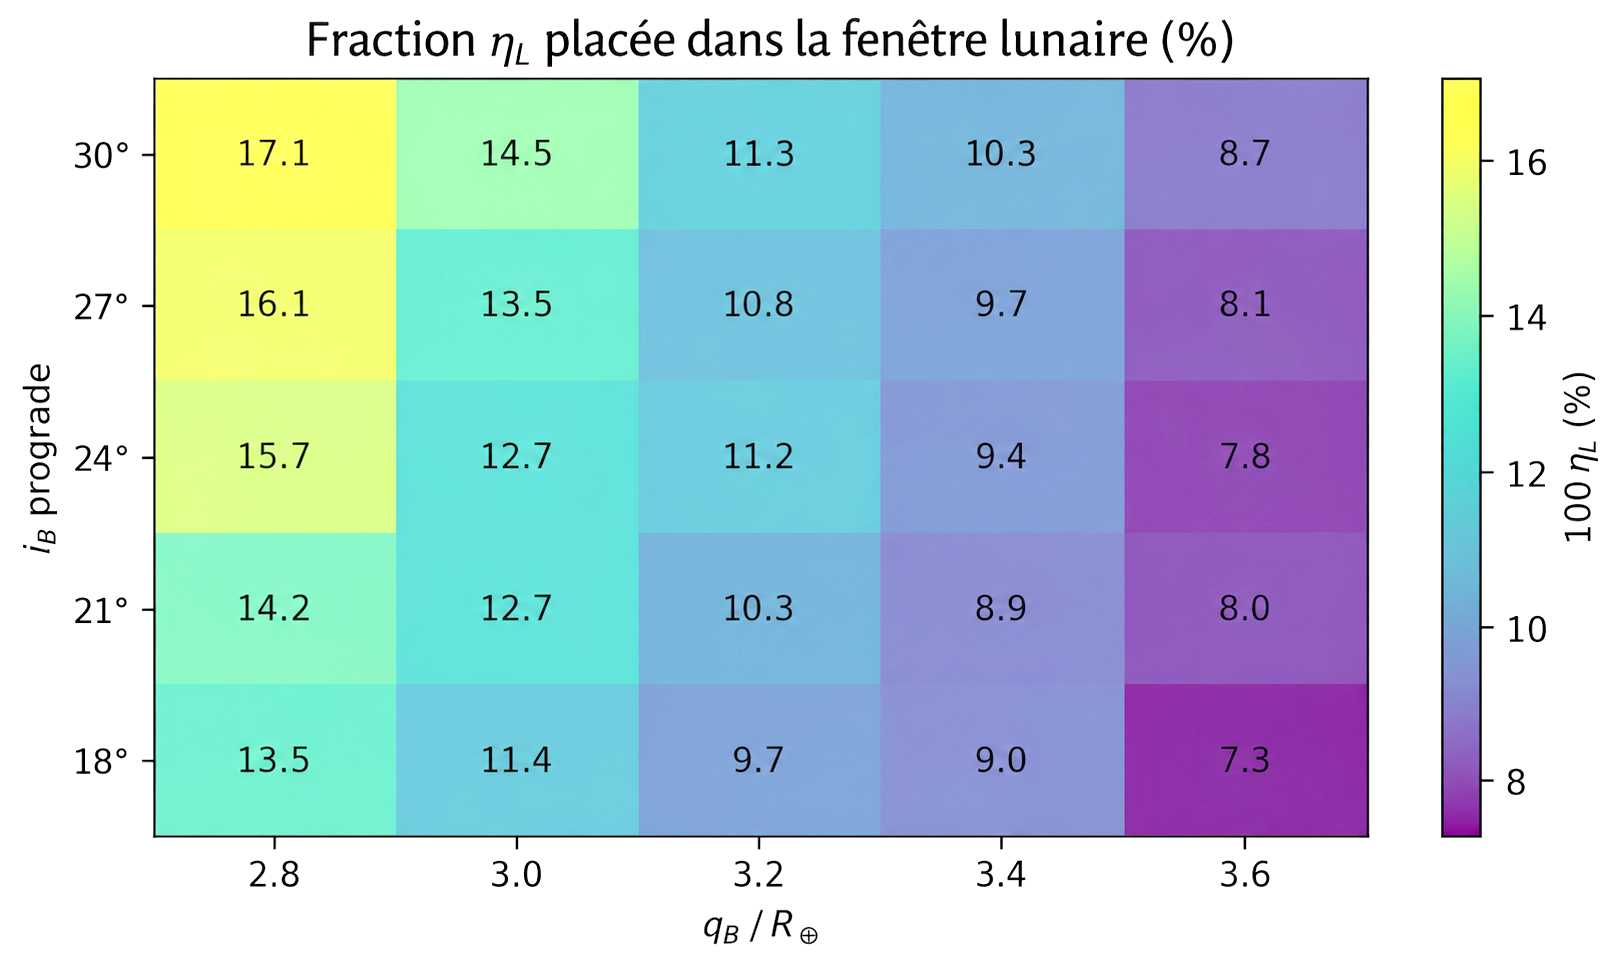
\includegraphics[width=0.82\textwidth]{Carte_etaL_pilote.png}
\caption{Carte pilote de $\eta_L(q_B,i_B)$ pour le cas $M_B=0{,}10\,\Mt$,
$v_\infty=2$~km\,s$^{-1}$ et $\omega_B=90^\circ$. La carte illustre l'existence d'une bande de
réponses continues, à confirmer par des simulations massives, collisionnelles et autogravitantes.}
\label{fig:pilote-etaL}
\end{figure}

Pour le cas $q_B=3\,\Rt$ et $i_B=30^\circ$, le calcul donne
\begin{equation}
\eta_L=0{,}145,\qquad \eta_{\mathrm{esc}}=0{,}023,\qquad
\eta_{\mathrm{reaccr}}=0{,}019,\qquad \eta_{\to B}=0{,}023.
\label{eq:pilote-cas}
\end{equation}
La fraction restante, $0{,}789$, demeure liée dans le domaine intérieur ou dans des états qui ne
satisfont pas immédiatement la fenêtre lunaire. À masse initiale fixée, la masse directement
placée dans la fenêtre est
\begin{equation}
M_{L,\mathrm{fenetre}}\simeq0{,}145\,M_{D,0},
\label{eq:MLfenetre}
\end{equation}
ce qui signifie qu'une masse lunaire immédiatement placée dans cette fenêtre demanderait
$M_{D,0}\simeq6{,}9\,M_L$ dans ce calcul test. Pour $q_B=2{,}8\,\Rt$ et $i_B=30^\circ$, la valeur
$\eta_L=0{,}171$ abaisse cette masse à $M_{D,0}\simeq5{,}85\,M_L$.

Le contrôle rétrograde isole le rôle du sens de passage. Pour $q_B=3\,\Rt$, à latitude de
périastre identique et avec les autres paramètres inchangés, on obtient
\begin{equation}
\eta_{L,\mathrm{retro}}\simeq0{,}027,
\label{eq:retro-pilote}
\end{equation}
soit une efficacité environ $5{,}4$ fois plus faible que dans le cas prograde. Ce résultat est cohérent
avec l'argument de durée de cohérence de l'équation~\eqref{eq:prograde}.

L'origine radiale de la matière promue confirme que le tri agit principalement sur la partie externe
du réservoir, voisine de Roche : pour le cas $q_B=3\,\Rt$, $i_B=30^\circ$, les contributions à la
cohorte $\eta_L$ proviennent à $35{,}0\,\%$ de l'anneau $2{,}53$--$2{,}71\,\Rt$ et à
$53{,}1\,\%$ de l'anneau $2{,}71$--$2{,}90\,\Rt$.

\begin{controle}
Ce calcul pilote ne ferme pas encore la théorie : il néglige la masse propre du réservoir, les chocs,
la viscosité, la pression, l'autogravité, les collisions mutuelles et l'aplatissement complet de la
proto-Terre. Il établit toutefois un résultat concret de Niveau~I : un passage prograde de $B$ peut
placer une fraction mesurable du réservoir préexistant dans la fenêtre lunaire sans transformer
l'essentiel du disque en matière échappée. La prochaine étape est de remplacer cette carte de
particules test par une carte massive et dissipative.
\end{controle}

\begin{falsif}
Si, sur l'ensemble de la grille, $\Delta\eta_L$ reste négligeable, ou n'augmente qu'au prix d'une
fraction échappée incompatible avec la masse du réservoir, le mécanisme de tri orbital est
insuffisant et la branche correspondante est exclue.
\end{falsif}

\begin{rappel}
Le domaine de viabilité fixe ce que le calcul doit démontrer. La dernière partie énonce ce que la
nature devrait montrer si la théorie est correcte, et comment le vérifier.
\end{rappel}

% =====================================================================
\part{Prédictions}
\label{part:predictions}
% =====================================================================

\noindent
Chaque prédiction est énoncée sous la même forme : ce que l'on doit observer \emph{si la théorie
est correcte}, puis \emph{comment le vérifier}, par la mesure d'échantillons lunaires ou par le
calcul. Les prédictions portent sur l'architecture, la composition, la chronologie et la dynamique.

% ---------------------------------------------------------------------
\chapter{Prédictions et vérifications}
\label{ch:predictions}
\label{sec:signatures}
% ---------------------------------------------------------------------

\begin{prediction}{P1. Un satellite dominant}
\sila Le réservoir trié et relaxé produit une masse satellitaire concentrée presque entièrement
dans un corps unique :
\begin{equation}
\mathcal{D}_{\mathrm{arch}}=\left\{\Theta_I:\ M_L\simeq M_{L,\mathrm{obs}},\
N_{\mathrm{sat,grand}}\simeq1,\ f_{\mathrm{dom}}\to1\right\}.
\label{eq:Darch}
\end{equation}
\verif Simulations à $N$ corps de la Phase~C, avec collisions et autogravité, à partir des
réservoirs réorganisés de la Phase~B ; suivi de $N_{\mathrm{sat}}$ et de $f_{\mathrm{dom}}$.
\end{prediction}

\begin{prediction}{P2. Une part négligeable de $B$}
\sila La fraction de matière lunaire issue de $B$,
\begin{equation}
f_B=\frac{M_{B\to L}}{M_L},
\label{eq:fB}
\end{equation}
est faible, et les compositions isotopiques de l'oxygène, du titane et du chrome de la Lune sont
indiscernables de celles de la Terre silicatée, dans les limites~\eqref{eq:bornefB}.
\verif Mesures isotopiques de haute précision sur des échantillons lunaires variés ; calcul de
$M_{B\to D}$ en Phase~B pour les passages avec $q_B$ proche de $d_{R,B}$.
\end{prediction}

\begin{prediction}{P3. Un tungstène terrestre}
\sila Après correction de l'accrétion tardive, $\varepsilon^{182}$W lunaire est identique à celui du
manteau terrestre, et le rapport Hf/W de la matière lunaire ne produit pas d'excès de $^{182}$W
incompatible avec l'instant $t_B$.
\verif Mesures de $\varepsilon^{182}$W et de Hf/W sur des roches lunaires à faible exposition
cosmique ; comparaison avec la chronologie de la Phase~A.
\end{prediction}

\begin{prediction}{P4. L'héritage de la ségrégation du noyau terrestre}
\sila Les appauvrissements lunaires en V, Cr et Mn reproduisent ceux du manteau terrestre, et le
rapport W/U lunaire est proche du rapport terrestre.
\verif Estimations de la composition du manteau lunaire à partir des basaltes et des roches
primitives ; expériences de partage métal--silicate à haute pression.
\end{prediction}

\begin{prediction}{P5. Une corrélation dynamique--chimique}
\sila Une même cohorte de matière porte simultanément une histoire orbitale et une composition :
\begin{equation}
(r_0,\lambda_\Omega,z)\longleftrightarrow(\varepsilon_{\mathrm{orb}},j_z,q_p,\mathbf{X}),
\label{eq:correlation}
\end{equation}
et le rapport W/V de la matière injectée~\eqref{eq:WV} reflète la profondeur et la latitude
arrachées.
\verif Suivi des étiquettes $(\lambda_\Omega,z)$ en Phase~B ; comparaison du W/V calculé avec les
rapports mesurés, normalisés à des éléments de même comportement.
\end{prediction}

\begin{prediction}{P6. Un réservoir de composition terrestre}
\sila Le réservoir circumterrestre préexistant est de nature silicatée terrestre, alimenté
principalement par la perte de masse équatoriale et les éjectas du manteau, et l'excès de FeO
lunaire est produit par les transformations internes au réservoir.
\verif Bilans de Phase~A sur les canaux~\eqref{eq:canaux} ; calcul de
$\boldsymbol{\Pi}_D$ et comparaison avec les teneurs lunaires en FeO et en sidérophiles.
\end{prediction}

\begin{prediction}{P7. Une inclinaison initiale non nulle}
\sila Un passage légèrement incliné donne au réservoir réorganisé un moment cinétique non
colinéaire avec le spin terrestre :
\begin{equation}
i_{D,1}=\arccos\!\left(\frac{\mathbf{L}_{D,1}\cdot\mathbf{S}_{\oplus,1}}
{|\mathbf{L}_{D,1}|\,|\mathbf{S}_{\oplus,1}|}\right).
\label{eq:inclinaison}
\end{equation}
Cette grandeur constitue une condition initiale de l'évolution maréale du système Terre--Lune,
dont l'inclinaison orbitale lunaire est l'une des énigmes classiques \cite{PahlevanMorbidelli2015}.
\verif Calcul de $i_{D,1}$ en Phase~B, puis intégration de l'évolution maréale jusqu'à l'orbite
actuelle.
\end{prediction}

\begin{prediction}{P8. Un moment cinétique compatible}
\sila Le moment cinétique du système Terre--réservoir laissé par le passage, $J_{\oplus D,1}$, est
compatible avec celui du système Terre--Lune, compte tenu de son évolution ultérieure.
\verif Fermeture du bilan~\eqref{eq:fermeture} en Phase~B ; comparaison de $J_{\oplus D,1}$ avec
$L_{\mathrm{EM}}$.
\end{prediction}

\begin{prediction}{P9. Un tri orbital efficace dans la bande dynamique de basses latitudes}
\sila Il existe une région continue de la bande dynamique de basses latitudes prograde où $\Delta\eta_L$ est
significatif et $\eta_{\mathrm{esc}}$ modéré, conformément à~\eqref{eq:fenetre-succes}.
\verif Cartes de viabilité de la Phase~B (chapitre~\ref{ch:programme}).
\end{prediction}

% =====================================================================
\begin{prediction}{P10. Un destin héliocentrique éliminé pour \texorpdfstring{$B$}{B}}
\sila La planète $B$ appartient à la population des corps planétaires primitifs ensuite éliminés :
\begin{equation}
B\in\mathcal{P}_{\mathrm{elim}},\qquad t_B<t_{\mathrm{ej}},
\label{eq:predB}
\end{equation}
et l'orbite héliocentrique post-passage $\mathcal{H}_{B,1}$ est compatible avec une diffusion
ultérieure vers une collision, une accrétion par une planète ou une éjection du Système solaire.
\verif Intégrations $N$-corps héliocentriques démarrant à $\mathcal{H}_{B,1}$, avec scénarios
d'instabilité précoce et tardive, et vérification que les architectures finales restent compatibles
avec le Système solaire actuel.
\end{prediction}

\chapter*{Conclusion générale}
\addcontentsline{toc}{part}{Conclusion générale}
\markboth{Conclusion générale}{Conclusion générale}
% =====================================================================

La question posée au début de cet ouvrage était celle d'un chemin : comment le système
Terre--Lune observé aujourd'hui a-t-il pu émerger du système proto-terrestre par une évolution
physiquement cohérente ?

La théorie propose une réponse précise. Pendant sa croissance, la proto-Terre est accompagnée
d'un réservoir secondaire circumterrestre, analogue par son principe aux systèmes d'accrétion des
planètes géantes et au disque de PDS~70c, mais dominé par les solides et alimenté principalement
par sa propre couche silicatée. Ce réservoir contient déjà de la masse et du moment cinétique
lorsque la planète $B$ passe.

$B$ n'est ni un impacteur ni un fournisseur principal de matière lunaire. C'est un agent
gravitationnel transitoire de redistribution des flux de masse et de moment cinétique entre les
réservoirs. Les passages rasants sont au moins aussi fréquents que les collisions
(équation~\eqref{eq:frequence}) ; la trajectoire de $B$ porte un moment cinétique de l'ordre de celui
du système Terre--Lune (équation~\eqref{eq:LBrel}) ; dans la bande dynamique de basses latitudes d'une proto-Terre
oblate en rotation rapide, son passage prograde injecte une matière superficielle déjà appauvrie
en métal. Son résultat central est un tri orbital : une cohorte liée est placée, par le couple de $B$,
dans la fenêtre lunaire au-delà de la limite de Roche (équations~\eqref{eq:fenetre}
et~\eqref{eq:etaL}), tandis que d'autres fractions réaccrètent ou s'échappent.

Le réservoir trié se relaxe et accrète la Lune, en concentrant la masse satellitaire dans un corps
dominant. La géochimie appartient à la même histoire : le passage non collisionnel favorise une
faible contribution de $B$, ce qui fait de la similitude isotopique une contrainte attendue du
domaine viable ; le vanadium et le tungstène, lus conjointement, tracent les flux de matière
silicatée terrestre et la profondeur de la couche prélevée.

La logique du modèle se referme avec le destin de $B$. L'agent qui réorganise le réservoir
circumterrestre n'a pas à demeurer dans le Système solaire final : il peut appartenir à la population
des corps planétaires primitifs ensuite éliminés par l'instabilité orbitale globale, pourvu que son
passage vérifie $t_B<t_{\mathrm{ej}}$. Cette hypothèse relie la formation Terre--Lune à la migration
et à l'instabilité du Système solaire primitif, sans imposer que $B$ soit identifié à une planète
manquante unique.

La question scientifique finale s'écrit
\begin{equation}
\boxed{\;\mathcal{S}_0=\{\Theta_I\}\longrightarrow\mathcal{D}_0
\xrightarrow{\;\text{tri orbital par }B\;}\mathcal{D}_1\longrightarrow
\left(M_L,\,L_L,\,i_{L,0},\,\mathbf{X}_L\right)\in\mathcal{D}_{\mathrm{viable}}
\longrightarrow\mathcal{S}_f.\;}
\label{eq:question}
\end{equation}
La théorie ne prétend pas démontrer une histoire unique. Elle définit un chemin physique
quantitatif et falsifiable, et elle indique, pour chacune de ses étapes, comment le confirmer, le
restreindre ou l'exclure.

% =====================================================================
\appendix
% =====================================================================

\chapter{Démonstrations}
\label{app:demo}

\section{Rayon de circularisation de la matière capturée}
\label{app:rc}

Une matière capturée à travers une zone d'accrétion de rayon $R_{\mathrm{acc}}$ dans un
écoulement cisaillé de fréquence $\Omega$ porte un moment cinétique spécifique d'ordre
$j\simeq\Omega R_{\mathrm{acc}}^2/4$ \cite{QuillenTrilling1998}. Elle se circularise au rayon où son
moment cinétique égale le moment képlérien, $j^2=G\Mt r_c$ :
\begin{equation}
r_c=\frac{\Omega^2R_{\mathrm{acc}}^4}{16\,G\Mt}.
\end{equation}
Pour $R_{\mathrm{acc}}=R_H$, la définition du rayon de Hill, $R_H^3=G\Mt/(3\Omega^2)$, donne
$\Omega^2=G\Mt/(3R_H^3)$ et $r_c=R_H/48$. Pour une accrétion limitée à la sphère de Bondi,
$r_c$ est multiplié par $(R_{\mathrm{B}}/R_H)^4$, ce qui conduit à l'équation~\eqref{eq:rc}.

\section{Fréquence des passages rasants}

Pour une trajectoire hyperbolique de paramètre d'impact $b$, la conservation du moment
cinétique et de l'énergie donne $b\,v_\infty=q\,v_p$ et $v_p^2=v_\infty^2+2G\Mtot/q$, d'où
\begin{equation}
b^2=q^2\left(1+\frac{2G\Mtot}{q\,v_\infty^2}\right),\qquad \sigma(q)=\pi b^2,
\end{equation}
qui est l'équation~\eqref{eq:sigma}. Avec $\Theta=2G\Mtot/(R_cv_\infty^2)$,
$\sigma(R_c)=\pi R_c^2(1+\Theta)$ et $\sigma(2R_c)=\pi R_c^2(4+2\Theta)$ ; le rapport
$[\sigma(2R_c)-\sigma(R_c)]/\sigma(R_c)=(3+\Theta)/(1+\Theta)$ décroît de 3 à 1 lorsque $\Theta$ croît
de 0 à l'infini.

\section{Nœuds de la trajectoire et non-traversée}

L'équation de la conique s'écrit $r=p/(1+e\cos\nu)$ avec $p=q(1+e)$. La trajectoire traverse le
plan de référence lorsque l'argument de latitude $\omega+\nu$ vaut $0$ ou $\pi$, soit $\nu=-\omega$ ou
$\nu=\pi-\omega$ ; les rayons correspondants sont $p/(1+e\cos\omega)$ et $p/(1-e\cos\omega)$, dont le
plus petit vaut $p/(1+e|\cos\omega|)$. C'est l'équation~\eqref{eq:nontraversee}.

\section{Rayon de circularisation et périgée}
\label{app:rcirc}

Pour une orbite liée, $j^2=G\Mt\,a(1-e^2)$ et $q_p=a(1-e)$, donc
$r_{\mathrm{circ}}=j^2/(G\Mt)=a(1-e)(1+e)=q_p(1+e)$. Comme $0\le e<1$,
$q_p\le r_{\mathrm{circ}}<2q_p$, ce qui établit l'équation~\eqref{eq:rcirc-qp}.

\section{Frontières du tri orbital}
\label{app:tri}

Un élément sur orbite circulaire de rayon $r_0$ a la vitesse $v_K=\sqrt{G\Mt/r_0}$. Après une
impulsion tangentielle, $v=v_K(1+\delta)$ et $j=r_0v_K(1+\delta)$, d'où
$r_{\mathrm{circ}}=r_0(1+\delta)^2$. Son énergie spécifique vaut
\begin{equation}
\varepsilon=\frac{G\Mt}{r_0}\left[\frac{(1+\delta)^2}{2}-1\right],
\end{equation}
qui s'annule pour $(1+\delta)^2=2$ : $\delta_{\mathrm{esc}}=\sqrt2-1$. Pour $\delta<0$, $r_0$ devient
l'apogée ; le demi-grand axe vaut $a=r_0/[2-(1+\delta)^2]$ et le périgée
$q_p=2a-r_0=r_0(1+\delta)^2/[2-(1+\delta)^2]$. La condition $q_p=\Req$ donne
$(1+\delta)^2=2\Req/(r_0+\Req)$, soit $\delta_{\mathrm{re}}$. La condition $r_{\mathrm{circ}}=\aR$
donne $\delta_L=\sqrt{\aR/r_0}-1$. On obtient l'équation~\eqref{eq:frontieres}.

\section{Impulsion de marée}
\label{app:impulsion}

Dans l'approximation d'une trajectoire rectiligne rapide de vitesse $V$ et de paramètre $b$, la
proto-Terre et un élément situé à la position relative $\mathbf{r}$ reçoivent des impulsions dont la
différence, au premier ordre en $r/b$, a une amplitude au plus d'ordre $2GM_Br/(b^2V)$
\cite{Spitzer1958,BinneyTremaine2008}. Avec $b=q_B$, $V=v_p=\sqrt{2G\Mtot/q_B}$ et
$v_K=\sqrt{G\Mt/r}$ :
\begin{equation}
\frac{\Delta v}{v_K}\sim\frac{2\mu_B\sqrt{G\Mt}\,r^{3/2}}{q_B^2v_p}
=\sqrt2\,\frac{\mu_B}{\sqrt{1+\mu_B}}\left(\frac{r}{q_B}\right)^{3/2}.
\end{equation}
Cette estimation suppose $r<q_B$ et un forçage impulsif ; elle néglige la courbure de la trajectoire
et donne donc un ordre de grandeur, que la Phase~B remplace par le calcul exact.

\section{Énergie de circularisation}

Une parcelle d'énergie $\varepsilon_i=-G\Mt/(2a)$ se circularise à moment cinétique conservé au
rayon $a_{\mathrm{circ}}=a(1-e^2)$, d'énergie $\varepsilon_f=-G\Mt/(2a_{\mathrm{circ}})$. L'énergie
libérée vaut
$\varepsilon_i-\varepsilon_f=\frac{G\Mt}{2a}\left[\frac{1}{1-e^2}-1\right]=\frac{G\Mt}{2a}\frac{e^2}{1-e^2}$,
ce qui est l'équation~\eqref{eq:circ}.

\section{Seuil d'injection}

Au point sous $B$, l'accélération de marée radiale vaut, lorsque $\lambda_B=0$,
\begin{equation}
GM_B\left[(q_B-\Req)^{-2}-q_B^{-2}\right]\simeq2GM_B\Req/q_B^3.
\end{equation}
À basse latitude, sa projection sur la direction radiale est multipliée par
$F(\lambda_B)=(3\cos^2\lambda_B-1)/2$. L'égaler à la gravité effective
$(G\Mt/\Req^2)(1-\tilde\omega^2)$ donne
\begin{equation}
1-\tilde\omega^2\lesssim2F(\lambda_B)\,\frac{M_B}{\Mt}\left(\frac{\Req}{q_B}\right)^3,
\end{equation}
qui est l'équation~\eqref{eq:seuil}.

\section{Borne sur la part chondritique du réservoir}
\label{app:borneW}

Avec $f_B=0$ et $\varepsilon^{182}\mathrm{W}_\oplus=0$, l'équation~\eqref{eq:melange} s'écrit
$\varepsilon^{182}\mathrm{W}_L=f_0C_{\mathrm{W},0}\varepsilon^{182}\mathrm{W}_0/
[f_0C_{\mathrm{W},0}+(1-f_0)C_{\mathrm{W},\oplus}]$. Pour $f_0C_{\mathrm{W},0}\ll C_{\mathrm{W},\oplus}$,
le dénominateur se réduit à $C_{\mathrm{W},\oplus}$, et la condition
$|\varepsilon^{182}\mathrm{W}_L|<\delta\varepsilon$ donne l'équation~\eqref{eq:bornef0}.

% ---------------------------------------------------------------------
\chapter{Notations}
\label{app:notations}
% ---------------------------------------------------------------------

\small
\begin{longtable}{>{\raggedright\arraybackslash}p{3.2cm}>{\raggedright\arraybackslash}p{11.6cm}}
\toprule
\textbf{Symbole} & \textbf{Signification} \\
\midrule
\endhead
$\mathcal{S}_0$, $\mathcal{S}_f$ & état initial du système proto-terrestre, état observé \\
$\RT$, $\RD$, $\RB$, $\Rinf$ & réservoirs : proto-Terre, réservoir circumterrestre, planète $B$, milieu extérieur \\
$\Phi_{i\to j}$ & flux de masse du réservoir $i$ vers le réservoir $j$ \\
$\boldsymbol{\mathcal{T}}_{j\to i}$ & couple exercé par le réservoir $j$ sur le réservoir $i$ \\
$\mathbf{X}_i$, $\mathbf{X}_{i\to j}$ & composition d'un réservoir, d'un flux \\
$\Mt$, $\Req$, $\Omega_\oplus$, $S_\oplus$ & masse, rayon équatorial, vitesse angulaire et spin de la proto-Terre \\
$\tilde\omega$ & rotation réduite $\Omega_\oplus/\sqrt{G\Mt/\Req^3}$ \\
$J_2$ & coefficient d'aplatissement gravitationnel \\
$M_D$, $L_D$, $\Sigma(r)$ & masse, moment cinétique et densité surfacique du réservoir \\
$\mathcal{D}_0$, $\mathcal{D}_1$ & état du réservoir avant et après la rencontre \\
$\mathcal{S}(t)$ & population d'agrégats et de lunules \\
$R_{\mathrm{in}}$, $R_{\mathrm{out}}$ & rayons interne et externe du réservoir \\
$R_H$, $R_{\mathrm{B}}$ & rayons de Hill et de Bondi \\
$\aR$, $a_{\mathrm{sync}}$ & limite de Roche, orbite synchrone \\
$M_B$, $\mu_B$, $R_B$, $\rho_B$ & masse, masse relative, rayon et densité de $B$ \\
$q_B$, $v_\infty$, $v_p$, $e_B$ & périastre, vitesse asymptotique, vitesse au périastre, excentricité de la trajectoire de $B$ \\
$i_B$, $\omega_B$ & inclinaison sur l'équateur rotationnel, argument du périastre \\
$\lambda_B$ & latitude du point sous $B$ au périastre \\
$\lambda_c$ & demi-largeur de la bande dynamique de basses latitudes \\
$t_{\mathrm{enc}}$, $\eta(r)$ & durée de la rencontre, paramètre de régime $\Omega_Kt_{\mathrm{enc}}$ \\
$d_{R,B}$ & distance de Roche de $B$ autour de la proto-Terre \\
$L_{B,\mathrm{rel}}$, $\chi_J$ & moment orbital relatif de $B$, fraction échangée \\
$\varepsilon$, $j$, $j_z$, $e$, $q_p$ & énergie, moment cinétique, projection, excentricité et périgée d'un élément \\
$r_{\mathrm{circ}}$ & rayon de circularisation $j^2/(G\Mt)$ \\
$\eta_L$, $\Delta\eta_L$ & fraction dans la fenêtre lunaire, contribution propre de $B$ \\
$\eta_{\mathrm{in}}$, $\eta_{\mathrm{reaccr}}$, $\eta_{\mathrm{esc}}$, $\eta_{\to B}$ & fractions : disque intérieur, réaccrétion, échappement, capture par $B$ \\
$\delta$ & impulsion tangentielle relative $\Delta v_t/v_K$ \\
$f_0$, $f_\oplus$, $f_B$ & fractions de provenance de la matière lunaire \\
$f_{\mathrm{dom}}$, $N_{\mathrm{sat}}$ & facteur de dominance, nombre de satellites \\
$\lambda_\Omega$, $z$ & latitude dynamique et profondeur d'origine de la matière injectée \\
$\mathcal{P}_{\mathrm{elim}}$ & population des corps planétaires primitifs ensuite éliminés par collision, accrétion, diffusion ou éjection \\
$t_{\mathrm{ej}}$ & instant d'éjection ou d'élimination dynamique de $B$ \\
$\mathcal{H}_{B,1}$ & orbite héliocentrique de $B$ après son passage près de la proto-Terre \\
$\Theta_I$ & vecteur des paramètres du Niveau I \\
$\mathcal{D}_{\mathrm{viable}}$ & domaine de viabilité \\
$\mathcal{D}_{B,\mathrm{hel}}$ & porte héliocentrique vérifiant le destin éliminé de $B$ \\
\bottomrule
\end{longtable}
\normalsize

% ---------------------------------------------------------------------
\chapter{Constantes et valeurs numériques}
\label{app:constantes}
% ---------------------------------------------------------------------

\begin{table}[htbp]
\centering
\small
\caption{Constantes et valeurs de référence utilisées dans l'ouvrage.}
\label{tab:constantes}
\begin{tabular}{lll}
\toprule
\textbf{Grandeur} & \textbf{Symbole} & \textbf{Valeur} \\
\midrule
Paramètre gravitationnel terrestre & $G\Mt$ & $3{,}986\times10^{14}$ m$^3$\,s$^{-2}$ \\
Masse de la Terre & $\Mt$ & $5{,}972\times10^{24}$ kg \\
Rayon terrestre moyen & $\Rt$ & $6{,}371\times10^{6}$ m \\
Masse de la Lune & $M_L$ & $7{,}342\times10^{22}$ kg \\
Masse du Soleil & $M_\odot$ & $1{,}989\times10^{30}$ kg \\
Unité astronomique & $a_\oplus$ & $1{,}496\times10^{11}$ m \\
Densité lunaire moyenne & $\rho_s$ & $3{,}34$ g\,cm$^{-3}$ \\
Densité terrestre moyenne & $\bar\rho_\oplus$ & $5{,}51$ g\,cm$^{-3}$ \\
Moment cinétique Terre--Lune & $L_{\mathrm{EM}}$ & $\approx3{,}5\times10^{34}$ kg\,m$^2$\,s$^{-1}$ \\
Limite de Roche ($\rho_s=3{,}34$) & $\aR$ & $\approx2{,}9\,\Rt$ \\
Demi-vie du $^{182}$Hf & $t_{1/2}$ & $8{,}9$ Ma \\
\bottomrule
\end{tabular}
\end{table}

\clearpage
\phantomsection
\addcontentsline{toc}{part}{Bibliographie}
\markboth{Bibliographie}{Bibliographie}
\begin{thebibliography}{99}
\small

\bibitem{Pringle1981} J.~E. Pringle, « Accretion discs in astrophysics », \emph{Annual Review of
Astronomy and Astrophysics}, 19 (1981), 137--160. doi:10.1146/annurev.aa.19.090181.001033.

\bibitem{JohansenLacerda2010} A. Johansen et P. Lacerda, « Prograde rotation of protoplanets by
accretion of pebbles in a gaseous environment », \emph{Monthly Notices of the Royal Astronomical
Society}, 404 (2010), 475--485. doi:10.1111/j.1365-2966.2010.16309.x.

\bibitem{Visser2020} R.~G. Visser, C.~W. Ormel, C. Dominik et S. Ida, « Spinning up planetary
bodies by pebble accretion », \emph{Icarus}, 335 (2020), 113380. doi:10.1016/j.icarus.2019.07.014.

\bibitem{Johansen2021} A. Johansen, T. Ronnet, M. Bizzarro, M. Schiller, M. Lambrechts,
Å. Nordlund et H. Lammer, « A pebble accretion model for the formation of the terrestrial planets
in the Solar System », \emph{Science Advances}, 7 (2021), eabc0444. doi:10.1126/sciadv.abc0444.

\bibitem{CanupWard2006} R.~M. Canup et W.~R. Ward, « A common mass scaling for satellite systems
of gaseous planets », \emph{Nature}, 441 (2006), 834--839. doi:10.1038/nature04860.

\bibitem{Toomre1964} A. Toomre, « On the gravitational stability of a disk of stars »,
\emph{The Astrophysical Journal}, 139 (1964), 1217--1238. doi:10.1086/147861.

\bibitem{Ida1997} S. Ida, R.~M. Canup et G.~R. Stewart, « Lunar accretion from an impact-generated
disk », \emph{Nature}, 389 (1997), 353--357. doi:10.1038/38669.

\bibitem{SalmonCanup2012} J. Salmon et R.~M. Canup, « Lunar accretion from a Roche-interior fluid
disk », \emph{The Astrophysical Journal}, 760 (2012), 83. doi:10.1088/0004-637X/760/1/83.

\bibitem{CanupWard2002} R.~M. Canup et W.~R. Ward, « Formation of the Galilean satellites:
conditions of accretion », \emph{The Astronomical Journal}, 124 (2002), 3404--3423.
doi:10.1086/344684.

\bibitem{Nimmo2026} F. Nimmo, R. Canup, Y. Fujii, A. Izidoro, J. Ji, W. McKinnon, O. Mousis,
C. Ormel, M. Ogihara, D. Stevenson et M. Blanc, « Origin and evolution of the Galilean satellites
within the Jovian system », \emph{Space Science Reviews}, 222 (2026), article~46.
doi:10.1007/s11214-026-01295-6.

\bibitem{Charnoz2010} S. Charnoz, J. Salmon et A. Crida, « The recent formation of Saturn's
moonlets from viscous spreading of the main rings », \emph{Nature}, 465 (2010), 752--754.
doi:10.1038/nature09096.

\bibitem{Blanc2025} M. Blanc, A. Crida, Y. Shibaike, S. Charnoz, M. El~Moutamid, P. Estrada,
O. Mousis, J. Salmon, A. Schneeberger et P. Vernazza, « Understanding the formation of Saturn's
regular moons in the context of giant planet moons formation scenarios », \emph{Space Science
Reviews}, 221 (2025), article~35. doi:10.1007/s11214-025-01156-8.

\bibitem{Helled2020} R. Helled, N. Nettelmann et T. Guillot, « Uranus and Neptune: origin,
evolution and internal structure », \emph{Space Science Reviews}, 216 (2020).
doi:10.1007/s11214-020-00660-3.

\bibitem{Benisty2021} M. Benisty, J. Bae, S. Facchini, M. Keppler, R. Teague, A. Isella,
N.~T. Kurtovic, L.~M. Pérez, A. Sierra, S.~M. Andrews et al., « A circumplanetary disk around
PDS70c », \emph{The Astrophysical Journal Letters}, 916 (2021), L2. doi:10.3847/2041-8213/ac0f83.

\bibitem{JPL} Jet Propulsion Laboratory, Solar System Dynamics, « Planetary satellite physical
parameters and mean elements », JPL/Caltech, données consultées en septembre 2026.

\bibitem{Popovas2018} A. Popovas, Å. Nordlund, J.~P. Ramsey et C.~W. Ormel, « Pebble dynamics and
accretion on to rocky planets -- I. Adiabatic and convective models », \emph{Monthly Notices of the
Royal Astronomical Society}, 479 (2018), 5136--5156. doi:10.1093/mnras/sty1752.

\bibitem{Ruskol1960} E.~L. Ruskol, « The origin of the Moon. I. Formation of a swarm of bodies
around the Earth », \emph{Soviet Astronomy}, 4 (1960), 657.

\bibitem{Weidenschilling1986} S.~J. Weidenschilling, R. Greenberg, C.~R. Chapman, F. Herbert,
D.~R. Davis, M.~J. Drake, J. Jones et W.~K. Hartmann, « Origin of the Moon from a circumterrestrial
disk », in W.~K. Hartmann, R.~J. Phillips et G.~J. Taylor (éds.), \emph{Origin of the Moon}, Lunar
and Planetary Institute, Houston (1986), 519--550.

\bibitem{HartmannDavis1975} W.~K. Hartmann et D.~R. Davis, « Satellite-sized planetesimals and
lunar origin », \emph{Icarus}, 24 (1975), 504--515.

\bibitem{CameronWard1976} A.~G.~W. Cameron et W.~R. Ward, « The origin of the Moon »,
\emph{Lunar Science VII} (1976), 120--122.

\bibitem{CanupAsphaug2001} R.~M. Canup et E. Asphaug, « Origin of the Moon in a giant impact near
the end of the Earth's formation », \emph{Nature}, 412 (2001), 708--712. doi:10.1038/35089010.

\bibitem{Canup2004} R.~M. Canup, « Simulations of a late lunar-forming impact », \emph{Icarus},
168 (2004), 433--456. doi:10.1016/j.icarus.2003.09.028.

\bibitem{CukStewart2012} M. Ćuk et S.~T. Stewart, « Making the Moon from a fast-spinning Earth:
a giant impact followed by resonant despinning », \emph{Science}, 338 (2012), 1047--1052.
doi:10.1126/science.1225542.

\bibitem{Canup2012} R.~M. Canup, « Forming a Moon with an Earth-like composition via a giant
impact », \emph{Science}, 338 (2012), 1052--1055. doi:10.1126/science.1226073.

\bibitem{Lock2018} S.~J. Lock, S.~T. Stewart, M.~I. Petaev, Z. Leinhardt, M.~T. Mace,
S.~B. Jacobsen et M. Ćuk, « The origin of the Moon within a terrestrial synestia », \emph{Journal
of Geophysical Research: Planets}, 123 (2018), 910--951. doi:10.1002/2017JE005333.

\bibitem{Mitler1975} H.~E. Mitler, « Formation of an iron-poor moon by partial capture, or: yet
another exotic theory of lunar origin », \emph{Icarus}, 24 (1975), 256--268.

\bibitem{QuillenTrilling1998} A.~C. Quillen et D.~E. Trilling, « Do proto-Jovian planets drive
outflows? », \emph{The Astrophysical Journal}, 508 (1998), 707--713.

\bibitem{MartinLubow2011} R.~G. Martin et S.~H. Lubow, « Tidal truncation of circumplanetary
discs », \emph{Monthly Notices of the Royal Astronomical Society}, 413 (2011), 1447--1461.

\bibitem{Ormel2015} C.~W. Ormel, J.-M. Shi et R. Kuiper, « Hydrodynamics of embedded planets' first
atmospheres -- II. A rapid recycling of atmospheric gas », \emph{Monthly Notices of the Royal
Astronomical Society}, 447 (2015), 3512--3525.

\bibitem{Fung2015} J. Fung, P. Artymowicz et Y. Wu, « The 3D flow field around an embedded
planet », \emph{The Astrophysical Journal}, 811 (2015), 101.

\bibitem{Daisaka2001} H. Daisaka, H. Tanaka et S. Ida, « Viscosity in a dense planetary ring with
self-gravitating particles », \emph{Icarus}, 154 (2001), 296--312.

\bibitem{Safronov1960} V.~S. Safronov, « On the gravitational instability in flattened systems with
axial symmetry and non-uniform rotation », \emph{Annales d'Astrophysique}, 23 (1960), 979.

\bibitem{GoldreichLyndenBell1965} P. Goldreich et D. Lynden-Bell, « Gravitational stability of
uniformly rotating disks », \emph{Monthly Notices of the Royal Astronomical Society}, 130 (1965),
97--124.

\bibitem{Kokubo2000} E. Kokubo, S. Ida et J. Makino, « Evolution of a circumterrestrial disk and
formation of a single moon », \emph{Icarus}, 148 (2000), 419--436.

\bibitem{PahlevanMorbidelli2015} K. Pahlevan et A. Morbidelli, « Collisionless encounters and the
origin of the lunar inclination », \emph{Nature}, 527 (2015), 492--494. doi:10.1038/nature16137.

\bibitem{Breslau2014} A. Breslau, M. Steinhausen, K. Vincke et S. Pfalzner, « Sizes of
protoplanetary discs after star-disc encounters », \emph{Astronomy \& Astrophysics}, 565 (2014),
A130.

\bibitem{Kruijer2015} T.~S. Kruijer, T. Kleine, M. Fischer-Gödde et P. Sprung, « Lunar tungsten
isotopic evidence for the late veneer », \emph{Nature}, 520 (2015), 534--537.
doi:10.1038/nature14360.

\bibitem{Touboul2015} M. Touboul, I.~S. Puchtel et R.~J. Walker, « Tungsten isotopic evidence for
disproportional late accretion to the Earth and Moon », \emph{Nature}, 520 (2015), 530--533.
doi:10.1038/nature14355.

\bibitem{Young2016} E.~D. Young, I.~E. Kohl, P.~H. Warren, D.~C. Rubie, S.~A. Jacobson et
A. Morbidelli, « Oxygen isotopic evidence for vigorous mixing during the Moon-forming giant
impact », \emph{Science}, 351 (2016), 493--496. doi:10.1126/science.aad0525.

\bibitem{Zhang2012} J. Zhang, N. Dauphas, A.~M. Davis, I. Leya et A. Fedkin, « The proto-Earth as
a significant source of lunar material », \emph{Nature Geoscience}, 5 (2012), 251--255.
doi:10.1038/ngeo1429.


\bibitem{Ringwood1990} A.~E. Ringwood, T. Kato, W. Hibberson et N. Ware, « High-pressure
geochemistry of Cr, V and Mn and implications for the origin of the Moon », \emph{Nature}, 347
(1990), 174--176. doi:10.1038/347174a0.

\bibitem{Drake1989} M.~J. Drake, H.~E. Newsom et C.~J. Capobianco, « V, Cr, and Mn in the Earth,
Moon, EPB, and SPB and the origin of the Moon: experimental studies », \emph{Geochimica et
Cosmochimica Acta}, 53 (1989), 2101--2111.

\bibitem{GessmannRubie2000} C.~K. Gessmann et D.~C. Rubie, « The origin of the depletions of V,
Cr and Mn in the mantles of the Earth and Moon », \emph{Earth and Planetary Science Letters}, 184
(2000), 95--107.

\bibitem{Newsom1986} H.~E. Newsom, « Constraints on the origin of the Moon from the abundance of
molybdenum and other siderophile elements », in W.~K. Hartmann, R.~J. Phillips et G.~J. Taylor
(éds.), \emph{Origin of the Moon}, Lunar and Planetary Institute, Houston (1986), 203--229.

\bibitem{Canup2023} R.~M. Canup, K. Righter, N. Dauphas et al., « Origin of the Moon »,
\emph{Reviews in Mineralogy and Geochemistry}, 89 (2023), 53--102. arXiv:2103.02045.

\bibitem{Spitzer1958} L. Spitzer, « Disruption of galactic clusters », \emph{The Astrophysical
Journal}, 127 (1958), 17--27.

\bibitem{BinneyTremaine2008} J. Binney et S. Tremaine, \emph{Galactic Dynamics}, 2\textsuperscript{e}
édition, Princeton University Press, Princeton (2008).

\bibitem{ToomreToomre1972} A. Toomre et J. Toomre, « Galactic bridges and tails », \emph{The
Astrophysical Journal}, 178 (1972), 623--666.


\bibitem{MosqueiraEstrada2003a} I. Mosqueira et P.~R. Estrada, « Formation of the regular
satellites of giant planets in an extended gaseous nebula I: Subnebula model and accretion of
satellites », \emph{Icarus}, 163 (2003), 198--231. doi:10.1016/S0019-1035(03)00076-9.

\bibitem{CridaCharnoz2012} A. Crida et S. Charnoz, « Formation of regular satellites from ancient
massive rings in the Solar System », \emph{Science}, 338 (2012), 1196--1199.
doi:10.1126/science.1226477.

\bibitem{AgnorHamilton2006} C.~B. Agnor et D.~P. Hamilton, « Neptune's capture of its moon Triton
in a binary--planet gravitational encounter », \emph{Nature}, 441 (2006), 192--194.
doi:10.1038/nature04792.

\bibitem{BanfieldMurray1992} D. Banfield et N. Murray, « A dynamical history of the inner
Neptunian satellites », \emph{Icarus}, 99 (1992), 390--401.
doi:10.1016/0019-1035(92)90155-Z.

\bibitem{Showalter2019} M.~R. Showalter, I. de Pater, J.~J. Lissauer et R.~S. French, « The
seventh inner moon of Neptune », \emph{Nature}, 566 (2019), 350--353.
doi:10.1038/s41586-019-0909-9.

\bibitem{Szulagyi2018} J. Szulágyi, M. Cilibrasi et L. Mayer, « In situ formation of icy moons of
Uranus and Neptune », \emph{The Astrophysical Journal Letters}, 868 (2018), L13.
doi:10.3847/2041-8213/aaeed6.

\bibitem{Davis2026} M.~R. Davis, M. Belyakov, I. Wong, Z. Milby et M.~E. Brown, « Neptune's Inner
Moons and Rings Are Exposed Icy Body Interiors », arXiv:2607.27481 (2026).


\bibitem{Tsiganis2005} K.~Tsiganis, R.~Gomes, A.~Morbidelli et H.~F. Levison, « Origin of the
orbital architecture of the giant planets of the Solar System », \emph{Nature}, 435 (2005),
459--461. doi:10.1038/nature03539.

\bibitem{Gomes2005} R.~Gomes, H.~F. Levison, K.~Tsiganis et A.~Morbidelli, « Origin of the
cataclysmic Late Heavy Bombardment period of the terrestrial planets », \emph{Nature}, 435
(2005), 466--469. doi:10.1038/nature03676.

\bibitem{Nesvorny2011} D.~Nesvorn\'y, « Young Solar System's fifth giant planet? »,
\emph{The Astrophysical Journal Letters}, 742 (2011), L22. doi:10.1088/2041-8205/742/2/L22.

\bibitem{NesvornyMorbidelli2012} D.~Nesvorn\'y et A.~Morbidelli, « Statistical study of the early
Solar System's instability with four, five, and six giant planets », \emph{The Astronomical
Journal}, 144 (2012), 117. doi:10.1088/0004-6256/144/4/117.

\bibitem{Liu2022} B.~Liu, S.~N. Raymond et S.~A. Jacobson, « Early Solar System instability
triggered by dispersal of the gaseous disk », \emph{Nature}, 604 (2022), 643--646.
doi:10.1038/s41586-022-04535-1.

\bibitem{Clement2018} M.~S. Clement, N.~A. Kaib, S.~N. Raymond et K.~J. Walsh, « Mars' growth
stunted by an early giant planet instability », \emph{Icarus}, 311 (2018), 340--356.
doi:10.1016/j.icarus.2018.04.008.

\end{thebibliography}

\end{document}
